\documentclass{report}

%%%%%%%%%%%%%%%%%%%%%%%%%%%%%%%%%
% PACKAGE IMPORTS
%%%%%%%%%%%%%%%%%%%%%%%%%%%%%%%%%


\usepackage[tmargin=2cm,rmargin=1in,lmargin=1in,margin=0.85in,bmargin=1.5cm,footskip=.2in]{geometry}
\usepackage{amsmath,amsfonts,amsthm,amssymb,mathtools}

% \usepackage[bb=dsserif]{mathalpha}
% \usepackage{bm}
\usepackage{dsfont}
\usepackage{bookmark} 
\usepackage{booktabs}
\usepackage{enumerate}
\usepackage[shortlabels]{enumitem}
\usepackage{hyperref,theoremref}
\usepackage[table]{xcolor}
\usepackage[most,many,breakable]{tcolorbox}
\usepackage{xcolor}
\usepackage{graphicx}
\graphicspath{ {./images/} }
\usepackage{varwidth}
\usepackage{varwidth}
\usepackage{etoolbox}
%\usepackage{authblk}
\usepackage{nameref}
\usepackage{multicol,array}
\usepackage{tikz-cd}
\usepackage{cancel}
\usepackage{pgfplots}
\pgfplotsset{compat=newest}
\usepgfplotslibrary{patchplots}
\usepackage{anyfontsize}
\usepackage{sectsty}
%\usepackage{import}
%\usepackage{xifthen}
%\usepackage{pdfpages}
%\usepackage{transparent}
\usepackage[nameinlink]{cleveref}
\usepackage{fancyhdr}


%%%%%%%%%%%%%%%%%%%%%%%%%%%%%%
% HEADER AND FOOTER
%%%%%%%%%%%%%%%%%%%%%%%%%%%%%%
\pagestyle{fancy}

% Clear all header and footer fields
\fancyhf{}

% Redefine the chaptermark
\renewcommand{\chaptermark}[1]{%
  \markboth{\thechapter.\ \MakeUppercase{#1}}{}%
}

% Chapter name on the left of the header
\fancyhead[L]{\leftmark}

% Section name on the right of the header
\fancyhead[R]{\rightmark}

% Page number on the bottom right in the format "- 34 -"
\fancyhead[C]{\raisebox{-0pt}{-\hspace{4pt}\thepage\hspace{4pt}-}}

% Line at the top of the header
\renewcommand{\headrulewidth}{0.0pt}

\fancypagestyle{plain}{%
  \fancyhf{} % clear all header and footer fields
  \renewcommand{\headrulewidth}{0pt} % remove the header rule
  \renewcommand{\footrulewidth}{0pt} % remove the footer rule
}
%%%%%%%%%%%%%%%%%%%%%%%%%%%%%%
% SELF MADE COLORS
%%%%%%%%%%%%%%%%%%%%%%%%%%%%%%

\usetikzlibrary{shapes.geometric}
\usetikzlibrary{calc}
\usepackage{anyfontsize}

\definecolor{myg}{RGB}{56, 140, 70}
\definecolor{myb}{RGB}{45, 111, 177}
\definecolor{myr}{RGB}{199, 68, 64}
\definecolor{mytheorembg}{HTML}{fdf8ea} %orange
\definecolor{mytheoremfr}{HTML}{f19000}
\definecolor{myexamplebg}{HTML}{F2FBF8}
\definecolor{myexamplefr}{HTML}{88D6D1}
\definecolor{myexampleti}{HTML}{2A7F7F}
\definecolor{mydefinitbg}{HTML}{F2F2F9} %blue
\definecolor{mydefinitfr}{HTML}{00007B} 
\definecolor{mypropbg}{RGB}{56, 140, 70} %green
\definecolor{mypropfr}{RGB}{56, 140, 70}
\definecolor{mylemmabg}{RGB}{169, 144, 126}
\definecolor{mylemmafr}{RGB}{169, 144, 126}
\definecolor{notesgreen}{RGB}{0,162,0}
\definecolor{myp}{RGB}{197, 92, 212}
\definecolor{mygr}{HTML}{2C3338}
\definecolor{myred}{RGB}{127,0,0}
\definecolor{myyellow}{RGB}{169,121,69}
\definecolor{OrangeRed}{HTML}{ED135A}
\definecolor{Dandelion}{HTML}{FDBC42}
\definecolor{light-gray}{gray}{0.95}
\definecolor{Emerald}{HTML}{00A99D}
\definecolor{RoyalBlue}{HTML}{0071BC}

% \definecolor{mydefnewbg}{HTML}{FFF0E0}
% \definecolor{mydefnewfr}{HTML}{FF9900}
\definecolor{myRoyalBlue}{RGB}{50,60,150}
\definecolor{myGreen}{RGB}{45,100,45}
\definecolor{mynavy}{RGB}{56, 102, 148} % RGB color model

%%%%%%%%%%%%%%%%%%%%%%%%%%%%%%
% HYPERREF SETUP
%%%%%%%%%%%%%%%%%%%%%%%%%%%%%%

\hypersetup{
	colorlinks=true,
	linkcolor=mynavy,
	citecolor=BurntOrange,
	bookmarksnumbered=true,
	bookmarksopen=true,
}

%%%%%%%%%%%%%%%%%%%%%%%%%%%%
% TCOLORBOX SETUPS
%%%%%%%%%%%%%%%%%%%%%%%%%%%%


%================================
% NEW DEFINITION BOX
%================================


\newtcbtheorem[number within=section]{definition}{Definition}
{%
    enhanced
    ,breakable
    ,colback = mydefinitbg
    ,frame hidden
    ,boxrule = 0sp
    ,borderline west = {2pt}{0pt}{mydefinitfr}
    ,sharp corners
    ,detach title
    ,before upper = \tcbtitle\par\smallskip
    ,coltitle = mydefinitfr!85!black
    ,fonttitle = \bfseries\sffamily
    ,description font = \mdseries
    ,separator sign none
    ,segmentation style={solid, mydefinitfr!85!black}
	,label type=definition
}
{th}

% \newtcbtheorem[number within=chapter]{definition}{Definition}
% {%
%     enhanced
%     ,breakable
%     ,colback = mydefinitbg
%     ,frame hidden
%     ,boxrule = 0sp
%     ,borderline west = {2pt}{0pt}{mydefinitfr}
%     ,sharp corners
%     ,detach title
%     ,before upper = \tcbtitle\par\smallskip
%     ,coltitle = mydefinitfr!85!black
%     ,fonttitle = \bfseries\sffamily
%     ,description font = \mdseries
%     ,separator sign none
%     ,segmentation style={solid, mydefinitfr!85!black}
% 	,label type=definition
% }
% {th}

\setlength{\parindent}{0.5cm}
%================================
% THEOREM BOX
%================================

\tcbuselibrary{theorems,skins,hooks}
\newtcbtheorem[use counter from=definition, number within=section]{theorem}{Theorem}
{%
	enhanced,
	breakable,
	colback = mytheorembg,
	frame hidden,
	boxrule = 0sp,
	borderline west = {2pt}{0pt}{mytheoremfr},
	sharp corners,
	detach title,
	before upper = \tcbtitle\par\smallskip,
	coltitle = mytheoremfr,
	fonttitle = \bfseries\sffamily,
	description font = \mdseries,
	separator sign none,
	segmentation style={solid, mytheoremfr},
	label type=theorem
}
{th}

% \tcbuselibrary{theorems,skins,hooks}
% \newtcbtheorem[number within=chapter]{theorem}{Theorem}
% {%
% 	enhanced,
% 	breakable,
% 	colback = mytheorembg,
% 	frame hidden,
% 	boxrule = 0sp,
% 	borderline west = {2pt}{0pt}{mytheoremfr},
% 	sharp corners,
% 	detach title,
% 	before upper = \tcbtitle\par\smallskip,
% 	coltitle = mytheoremfr,
% 	fonttitle = \bfseries\sffamily,
% 	description font = \mdseries,
% 	separator sign none,
% 	segmentation style={solid, mytheoremfr},
% 	label type=theorem
% }
% {th}


\tcbuselibrary{theorems,skins,hooks}
\newtcolorbox{Theoremcon}
{%
	enhanced
	,breakable
	,colback = mytheorembg
	,frame hidden
	,boxrule = 0sp
	,borderline west = {2pt}{0pt}{mytheoremfr}
	,sharp corners
	,description font = \mdseries
	,separator sign none
}


%================================
% Corollery
%================================
\tcbuselibrary{theorems,skins,hooks}
\newtcbtheorem[use counter from=definition, number within=section]{corollary}{Corollary}
{%
	enhanced
	,breakable
	,colback = myp!10
	,frame hidden
	,boxrule = 0sp
	,borderline west = {2pt}{0pt}{myp!85!black}
	,sharp corners
	,detach title
	,before upper = \tcbtitle\par\smallskip
	,coltitle = myp!85!black
	,fonttitle = \bfseries\sffamily
	,description font = \mdseries
	,separator sign none
	,segmentation style={solid, myp!85!black}
	,label type=corollary
}
{th}
% \tcbuselibrary{theorems,skins,hooks}
% \newtcbtheorem[number within=chapter]{corollary}{Corollary}
% {%
% 	enhanced
% 	,breakable
% 	,colback = myp!10
% 	,frame hidden
% 	,boxrule = 0sp
% 	,borderline west = {2pt}{0pt}{myp!85!black}
% 	,sharp corners
% 	,detach title
% 	,before upper = \tcbtitle\par\smallskip
% 	,coltitle = myp!85!black
% 	,fonttitle = \bfseries\sffamily
% 	,description font = \mdseries
% 	,separator sign none
% 	,segmentation style={solid, myp!85!black}
% 	,label type=corol
% }
% {th}

%================================
% CLAIM
%================================

\tcbuselibrary{theorems,skins,hooks}
\newtcbtheorem[number within=section]{claim}{Claim}
{%
	enhanced
	,breakable
	,colback = myg!10
	,frame hidden
	,boxrule = 0sp
	,borderline west = {2pt}{0pt}{myg}
	,sharp corners
	,detach title
	,before upper = \tcbtitle\par\smallskip
	,coltitle = myg!85!black
	,fonttitle = \bfseries\sffamily
	,description font = \mdseries
	,separator sign none
	,segmentation style={solid, myg!85!black}
	,label type=claim
}
{th}


\newtcbtheorem[number within=chapter]{Claim}{Claim}
{%
	enhanced
	,breakable
	,colback = myg!10
	,frame hidden
	,boxrule = 0sp
	,borderline west = {2pt}{0pt}{myg}
	,sharp corners
	,detach title
	,before upper = \tcbtitle\par\smallskip
	,coltitle = myg!85!black
	,fonttitle = \bfseries\sffamily
	,description font = \mdseries
	,separator sign none
	,segmentation style={solid, myg!85!black}
	,label type=claim
}
{th}
%================================
% PROPOSITION
%================================

\tcbuselibrary{theorems,skins,hooks}
\newtcbtheorem[use counter from=definition, number within=section]{proposition}{Proposition}
{%
	enhanced
	,breakable
	,colback = mypropbg!10
	,frame hidden
	,boxrule = 0sp
	,borderline west = {2pt}{0pt}{mypropfr!85!black}
	,sharp corners
	,detach title
	,before upper = \tcbtitle\par\smallskip
	,coltitle = mypropfr!85!black
	,fonttitle = \bfseries\sffamily
	,description font = \mdseries
	,separator sign none
	,segmentation style={solid, mypropfr!85!black}
	,label type=proposition
}
{th}

% \newtcbtheorem[number within=chapter]{Proposition}{Proposition}
% {%
% 	enhanced
% 	,breakable
% 	,colback = mypropbg!10
% 	,frame hidden
% 	,boxrule = 0sp
% 	,borderline west = {2pt}{0pt}{mypropfr!85!black}
% 	,sharp corners
% 	,detach title
% 	,before upper = \tcbtitle\par\smallskip
% 	,coltitle = mypropfr!85!black
% 	,fonttitle = \bfseries\sffamily
% 	,description font = \mdseries
% 	,separator sign none
% 	,segmentation style={solid, mypropfr!85!black}
% 	,label type=proposition
% }
% {th}
%================================
% LEMMA
%================================

\tcbuselibrary{theorems,skins,hooks}
\newtcbtheorem[use counter from=definition, number within=section]{lemma}{Lemma}
{%
	enhanced
	,breakable
	,colback = mylemmabg!10
	,frame hidden
	,boxrule = 0sp
	,borderline west = {2pt}{0pt}{mylemmafr!85!black}
	,sharp corners
	,detach title
	,before upper = \tcbtitle\par\smallskip
	,coltitle = mylemmafr!85!black
	,fonttitle = \bfseries\sffamily
	,description font = \mdseries
	,separator sign none
	,segmentation style={solid, mylemmafr!85!black}
	,label type=lemma
}
{th}

% \newtcbtheorem[number within=chapter]{Lemma}{Lemma}
% {%
% 	enhanced
% 	,breakable
% 	,colback = mylemmabg!10
% 	,frame hidden
% 	,boxrule = 0sp
% 	,borderline west = {2pt}{0pt}{mylemmafr!85!black}
% 	,sharp corners
% 	,detach title
% 	,before upper = \tcbtitle\par\smallskip
% 	,coltitle = mylemmafr!85!black
% 	,fonttitle = \bfseries\sffamily
% 	,description font = \mdseries
% 	,separator sign none
% 	,segmentation style={solid, mylemmafr!85!black}
% 	,label type=lemma
% }
% {th}
%================================
% EXAMPLE BOX
%================================

\newtcbtheorem[number within=section]{example}{Example}
{%
	colback = myexamplebg
	,breakable
	,colframe = myexamplefr
	,coltitle = myexampleti
	,boxrule = 1pt
	,sharp corners
	,detach title
	,before upper=\tcbtitle\par\smallskip
	,fonttitle = \bfseries\sffamily
	%,fonttitle = \bfseries
	,description font = \mdseries\sffamily
	%,description font = \mdseries
	,separator sign none
	%,description delimiters parenthesis
	,label type=example
}
{ex}

% \newtcbtheorem[number within=chapter]{example}{Example}
% {%
% 	colback = myexamplebg
% 	,breakable
% 	,colframe = myexamplefr
% 	,coltitle = myexampleti
% 	,boxrule = 1pt
% 	,sharp corners
% 	,detach title
% 	,before upper=\tcbtitle\par\smallskip
% 	,fonttitle = \bfseries
% 	,description font = \mdseries
% 	,separator sign none
% 	,description delimiters parenthesis
% 	,label type=example
% }
% {ex}

%================================
% DEFINITION BOX
%================================

% \newtcbtheorem[number within=section]{Definition}{Definition}{enhanced,
% 	before skip=2mm,after skip=2mm, colback=red!5,colframe=red!80!black,boxrule=0.5mm,
% 	attach boxed title to top left={xshift=1cm,yshift*=1mm-\tcboxedtitleheight}, varwidth boxed title*=-3cm,
% 	boxed title style={frame code={
% 					\path[fill=tcbcolback]
% 					([yshift=-1mm,xshift=-1mm]frame.north west)
% 					arc[start angle=0,end angle=180,radius=1mm]
% 					([yshift=-1mm,xshift=1mm]frame.north east)
% 					arc[start angle=180,end angle=0,radius=1mm];
% 					\path[left color=tcbcolback!60!black,right color=tcbcolback!60!black,
% 						middle color=tcbcolback!80!black]
% 					([xshift=-2mm]frame.north west) -- ([xshift=2mm]frame.north east)
% 					[rounded corners=1mm]-- ([xshift=1mm,yshift=-1mm]frame.north east)
% 					-- (frame.south east) -- (frame.south west)
% 					-- ([xshift=-1mm,yshift=-1mm]frame.north west)
% 					[sharp corners]-- cycle;
% 				},interior engine=empty,
% 		},
% 	fonttitle=\bfseries,
% 	title={#2},#1}{def}
% \newtcbtheorem[number within=chapter]{definition}{Definition}{enhanced,
% 	before skip=2mm,after skip=2mm, colback=red!5,colframe=red!80!black,boxrule=0.5mm,
% 	attach boxed title to top left={xshift=1cm,yshift*=1mm-\tcboxedtitleheight}, varwidth boxed title*=-3cm,
% 	boxed title style={frame code={
% 					\path[fill=tcbcolback]
% 					([yshift=-1mm,xshift=-1mm]frame.north west)
% 					arc[start angle=0,end angle=180,radius=1mm]
% 					([yshift=-1mm,xshift=1mm]frame.north east)
% 					arc[start angle=180,end angle=0,radius=1mm];
% 					\path[left color=tcbcolback!60!black,right color=tcbcolback!60!black,
% 						middle color=tcbcolback!80!black]
% 					([xshift=-2mm]frame.north west) -- ([xshift=2mm]frame.north east)
% 					[rounded corners=1mm]-- ([xshift=1mm,yshift=-1mm]frame.north east)
% 					-- (frame.south east) -- (frame.south west)
% 					-- ([xshift=-1mm,yshift=-1mm]frame.north west)
% 					[sharp corners]-- cycle;
% 				},interior engine=empty,
% 		},
% 	fonttitle=\bfseries,
% 	title={#2},#1}{def}



%================================
% OPEN QUESTION BOX
%================================

\newtcbtheorem[number within=section]{open}{Open Question}{enhanced,
	before skip=2mm,after skip=2mm, colback=myp!5,colframe=myp!80!black,boxrule=0.5mm,
	attach boxed title to top left={xshift=1cm,yshift*=1mm-\tcboxedtitleheight}, varwidth boxed title*=-3cm,
	boxed title style={frame code={
			\path[fill=tcbcolback]
			([yshift=-1mm,xshift=-1mm]frame.north west)
			arc[start angle=0,end angle=180,radius=1mm]
			([yshift=-1mm,xshift=1mm]frame.north east)
			arc[start angle=180,end angle=0,radius=1mm];
			\path[left color=tcbcolback!60!black,right color=tcbcolback!60!black,
			middle color=tcbcolback!80!black]
			([xshift=-2mm]frame.north west) -- ([xshift=2mm]frame.north east)
			[rounded corners=1mm]-- ([xshift=1mm,yshift=-1mm]frame.north east)
			-- (frame.south east) -- (frame.south west)
			-- ([xshift=-1mm,yshift=-1mm]frame.north west)
			[sharp corners]-- cycle;
		},interior engine=empty,
	},
	fonttitle=\bfseries,
	title={#2},#1}{def}
\newtcbtheorem[number within=chapter]{Open}{Open Question}{enhanced,
	before skip=2mm,after skip=2mm, colback=myp!5,colframe=myp!80!black,boxrule=0.5mm,
	attach boxed title to top left={xshift=1cm,yshift*=1mm-\tcboxedtitleheight}, varwidth boxed title*=-3cm,
	boxed title style={frame code={
			\path[fill=tcbcolback]
			([yshift=-1mm,xshift=-1mm]frame.north west)
			arc[start angle=0,end angle=180,radius=1mm]
			([yshift=-1mm,xshift=1mm]frame.north east)
			arc[start angle=180,end angle=0,radius=1mm];
			\path[left color=tcbcolback!60!black,right color=tcbcolback!60!black,
			middle color=tcbcolback!80!black]
			([xshift=-2mm]frame.north west) -- ([xshift=2mm]frame.north east)
			[rounded corners=1mm]-- ([xshift=1mm,yshift=-1mm]frame.north east)
			-- (frame.south east) -- (frame.south west)
			-- ([xshift=-1mm,yshift=-1mm]frame.north west)
			[sharp corners]-- cycle;
		},interior engine=empty,
	},
	fonttitle=\bfseries,
	title={#2},#1}{def}



%================================
% EXERCISE BOX
%================================

\makeatletter
\newtcbtheorem{question}{Question}{enhanced,
	breakable,
	colback=white,
	colframe=myb!80!black,
	attach boxed title to top left={yshift*=-\tcboxedtitleheight},
	fonttitle=\bfseries,
	title={#2},
	boxed title size=title,
	boxed title style={%
			sharp corners,
			rounded corners=northwest,
			colback=tcbcolframe,
			boxrule=0pt,
		},
	underlay boxed title={%
			\path[fill=tcbcolframe] (title.south west)--(title.south east)
			to[out=0, in=180] ([xshift=5mm]title.east)--
			(title.center-|frame.east)
			[rounded corners=\kvtcb@arc] |-
			(frame.north) -| cycle;
		},
	#1
}{def}
\makeatother

%================================
% SOLUTION BOX
%================================

\makeatletter
\newtcolorbox{solution}{enhanced,
	breakable,
	colback=white,
	colframe=myg!80!black,
	attach boxed title to top left={yshift*=-\tcboxedtitleheight},
	title=Solution,
	boxed title size=title,
	boxed title style={%
			sharp corners,
			rounded corners=northwest,
			colback=tcbcolframe,
			boxrule=0pt,
		},
	underlay boxed title={%
			\path[fill=tcbcolframe] (title.south west)--(title.south east)
			to[out=0, in=180] ([xshift=5mm]title.east)--
			(title.center-|frame.east)
			[rounded corners=\kvtcb@arc] |-
			(frame.north) -| cycle;
		},
}
\makeatother

%================================
% Question BOX
%================================

\makeatletter
\newtcbtheorem{qstion}{Question}{enhanced,
	breakable,
	colback=white,
	colframe=mygr,
	attach boxed title to top left={yshift*=-\tcboxedtitleheight},
	fonttitle=\bfseries,
	title={#2},
	boxed title size=title,
	boxed title style={%
			sharp corners,
			rounded corners=northwest,
			colback=tcbcolframe,
			boxrule=0pt,
		},
	underlay boxed title={%
			\path[fill=tcbcolframe] (title.south west)--(title.south east)
			to[out=0, in=180] ([xshift=5mm]title.east)--
			(title.center-|frame.east)
			[rounded corners=\kvtcb@arc] |-
			(frame.north) -| cycle;
		},
	#1
}{def}
\makeatother

\newtcbtheorem[number within=chapter]{wconc}{Wrong Concept}{
	breakable,
	enhanced,
	colback=white,
	colframe=myr,
	arc=0pt,
	outer arc=0pt,
	fonttitle=\bfseries\sffamily\large,
	colbacktitle=myr,
	attach boxed title to top left={},
	boxed title style={
			enhanced,
			skin=enhancedfirst jigsaw,
			arc=3pt,
			bottom=0pt,
			interior style={fill=myr}
		},
	#1
}{def}



%================================
% NOTE BOX
%================================

\usetikzlibrary{arrows,calc,shadows.blur}
\tcbuselibrary{skins}
\newtcolorbox{note}[1][]{%
	enhanced jigsaw,
	colback=gray!20!white,%
	colframe=gray!80!black,
	size=small,
	boxrule=1pt,
	title=\textbf{Note:-},
	halign title=flush center,
	coltitle=black,
	breakable,
	drop shadow=black!50!white,
	attach boxed title to top left={xshift=1cm,yshift=-\tcboxedtitleheight/2,yshifttext=-\tcboxedtitleheight/2},
	minipage boxed title=1.5cm,
	boxed title style={%
			colback=white,
			size=fbox,
			boxrule=1pt,
			boxsep=2pt,
			underlay={%
					\coordinate (dotA) at ($(interior.west) + (-0.5pt,0)$);
					\coordinate (dotB) at ($(interior.east) + (0.5pt,0)$);
					\begin{scope}
						\clip (interior.north west) rectangle ([xshift=3ex]interior.east);
						\filldraw [white, blur shadow={shadow opacity=60, shadow yshift=-.75ex}, rounded corners=2pt] (interior.north west) rectangle (interior.south east);
					\end{scope}
					\begin{scope}[gray!80!black]
						\fill (dotA) circle (2pt);
						\fill (dotB) circle (2pt);
					\end{scope}
				},
		},
	#1,
}

%%%%%%%%%%%%%%%%%%%%%%%%%%%%%%
% SELF MADE COMMANDS
%%%%%%%%%%%%%%%%%%%%%%%%%%%%%%

\NewDocumentCommand{\EqM}{ m O{black} m}{%
	\tikz[remember picture, baseline, anchor=base] 
	\node[inner sep=0pt, outer sep=3pt, text=#2] (#1) {%
		\ensuremath{#3}%
	};    
}

% \newcommand{\thm}[3][]{\begin{theorem}{#2}{#1}#3\end{theorem}}
% \newcommand{\thmc}[3][]{\begin{theorem}{#2}{#1}#3\end{theorem}}
% \newcommand{\cor}[3][]{\begin{corollary}{#2}{#1}#3\end{corollary}}
% \newcommand{\corc}[3][]{\begin{corollary}{#2}{#1}#3\end{corollary}}
% \newcommand{\clm}[3][]{\begin{claim}{#2}{#1}#3\end{claim}}
% \newcommand{\prop}[3][]{\begin{proposition}{#2}{#1}#3\end{proposition}}
% \newcommand{\lemm}[3][]{\begin{lemma}{#2}{#1}#3\end{lemma}}
% \newcommand{\wc}[3][]{\begin{wconc}{#2}{#1}\setlength{\parindent}{1cm}#3\end{wconc}}
% \newcommand{\thmcon}[1]{\begin{Theoremcon}{#1}\end{Theoremcon}}
% \newcommand{\ex}[3][]{\begin{example}{#2}{#1}#3\end{example}}
% \newcommand{\exc}[3][]{\begin{example}{#2}{#1}#3\end{example}}
% \newcommand{\dfn}[3][]{\begin{definition}{#2}{#1}#3\end{definition}}
% \newcommand{\dfn}[3][]{\begin{Definition}[colbacktitle=red!75!black]{#2}{#1}#3\end{Definition}}
% \newcommand{\dfnc}[3][]{\begin{definition}[colbacktitle=red!75!black]{#2}{#1}#3\end{definition}}
% \newcommand{\opn}[3][]{\begin{open}[colbacktitle=myp!75!black]{#2}{#1}#3\end{open}}
% \newcommand{\opnc}[3][]{\begin{Open}[colbacktitle=myp!75!black]{#2}{#1}#3\end{Open}}
% \newcommand{\qs}[3][]{\begin{question}{#2}{#1}#3\end{question}}
%\newcommand{\pf}[2]{\begin{myproof}[#1]#2\end{myproof}}
% \newcommand{\pf}[2][Proof]{\begin{prf}[#1]#2\end{prf}}
% \newcommand{\nt}[1]{\begin{note}#1\end{note}}

\newcommand*\circled[1]{\tikz[baseline=(char.base)]{
		\node[shape=circle,draw,inner sep=1pt] (char) {#1};}}
\newcommand\getcurrentref[1]{%
	\ifnumequal{\value{#1}}{0}
	{??}
	{\the\value{#1}}%
}
\newcommand{\getCurrentSectionNumber}{\getcurrentref{section}}
\newenvironment{prf}[1][\proofname]{%
	\proof[#1.]%
}{\endproof}
\newcounter{mylabelcounter}

\makeatletter
\newcommand{\setword}[2]{%
	\phantomsection
	#1\def\@currentlabel{\unexpanded{#1}}\label{#2}%
}
\makeatother

\newenvironment{remark}[1][Remark]{%
    \par\noindent\textit{#1.}\hspace{1ex}%
}{\qed\par}


\tikzset{
	symbol/.style={
			draw=none,
			every to/.append style={
					edge node={node [sloped, allow upside down, auto=false]{$#1$}}}
		}
}

%\usepackage{framed}
%\usepackage{titletoc}
%\usepackage{etoolbox}
%\usepackage{lmodern}


%\patchcmd{\tableofcontents}{\contentsname}{\sffamily\contentsname}{}{}

%\renewenvironment{leftbar}
%{\def\FrameCommand{\hspace{6em}%
%		{\color{myyellow}\vrule width 2pt depth 6pt}\hspace{1em}}%
%	\MakeFramed{\parshape 1 0cm \dimexpr\textwidth-6em\relax\FrameRestore}\vskip2pt%
%}
%{\endMakeFramed}

%\titlecontents{chapter}
%[0em]{\vspace*{2\baselineskip}}
%{\parbox{4.5em}{%
%		\hfill\Huge\sffamily\bfseries\color{myred}\thecontentspage}%
%	\vspace*{-2.3\baselineskip}\leftbar\textsc{\small\chaptername~\thecontentslabel}\\\sffamily}
%{}{\endleftbar}
%\titlecontents{section}
%[8.4em]
%{\sffamily\contentslabel{3em}}{}{}
%{\hspace{0.5em}\nobreak\itshape\color{myred}\contentspage}
%\titlecontents{subsection}
%[8.4em]
%{\sffamily\contentslabel{3em}}{}{}  
%{\hspace{0.5em}\nobreak\itshape\color{myred}\contentspage}



%%%%%%%%%%%%%%%%%%%%%%%%%%%%%%%%%%%%%%%%%%%
% TABLE OF CONTENTS
%%%%%%%%%%%%%%%%%%%%%%%%%%%%%%%%%%%%%%%%%%%


\usepackage{titletoc}
\usepackage{sectsty} % For customizing section titles if needed

\renewcommand{\contentsname}{\fontfamily{times}\selectfont\Huge\bfseries\sffamily Contents}

% Define custom colors as per tstextbook.cls
\definecolor{tssteelblue}{RGB}{70,130,180}
\definecolor{tsorange}{RGB}{255,138,88}

% Customizing the Table of Contents

\contentsmargin{1cm}

% Chapter titles
\titlecontents{chapter}[0.25cm]
{\addvspace{2ex}\Large\bfseries\sffamily} % Spacing and font adjustments before the entry
{\hypersetup{linkcolor=tssteelblue}\color{tssteelblue}\contentslabel[\Large\thecontentslabel]{1.0cm}} % Label (number) formatting
{\hypersetup{linkcolor=tssteelblue}} % For unnumbered chapters
{\color{tssteelblue}\titlerule*[1pc]{.}\contentspage} % Dot leader and page number

% Section titles
\titlecontents{section}[1.5cm] % Indentation
{\addvspace{0.7ex}\large\bfseries\sffamily} % Spacing and font adjustments before the entry
{\hypersetup{linkcolor=black}\contentslabel[\thecontentslabel]{1.25cm}} % Label (number) formatting
{}
{\sffamily\hfill\color{black}\contentspage}[]

\titlecontents{subsection}[2.65cm] % Adjust the left margin to align with subsection indent
{\addvspace{0.25em}\sffamily}
{\hypersetup{linkcolor=black!85}\contentslabel[\thecontentslabel]{3.2em}} % Subsection label formatting
{} % Unnumbered format
{\hfill\color{black}\contentspage} % Page number


% \usepackage{tikz}
% \definecolor{doc}{RGB}{0,60,110}
% \usepackage{titletoc}
% \contentsmargin{0cm}
% \titlecontents{chapter}[3.7pc]
% {\addvspace{30pt}%
% 	\begin{tikzpicture}[remember picture, overlay]%
% 		\draw[fill=doc!60,draw=doc!60] (-7,-.1) rectangle (-0.7,.5);%
% 		\pgftext[left,x=-3.6cm,y=0.2cm]{\color{white}\Large\sc\bfseries Chapter\ \thecontentslabel};%
% 	\end{tikzpicture}\color{doc!60}\large\sc\bfseries}%
% {}
% {}
% {\;\titlerule\;\large\sc\bfseries Page \thecontentspage
% 	\begin{tikzpicture}[remember picture, overlay]
% 		\draw[fill=doc!60,draw=doc!60] (2pt,0) rectangle (4,0.1pt);
% 	\end{tikzpicture}}%
% \titlecontents{section}[3.7pc]
% {\addvspace{2pt}}
% {\contentslabel[\thecontentslabel]{2pc}}
% {}
% {\hfill\small \thecontentspage}
% []
% \titlecontents*{subsection}[3.7pc]
% {\addvspace{-1pt}\small}
% {}
% {}
% {\ --- \small\thecontentspage}
% [ \textbullet\ ][]

% \makeatletter
% \renewcommand{\tableofcontents}{%
% 	\chapter*{%
% 	  \vspace*{-20\p@}%
% 	  \begin{tikzpicture}[remember picture, overlay]%
% 		  \pgftext[right,x=15cm,y=0.2cm]{\color{doc!60}\Huge\sc\bfseries \contentsname};%
% 		  \draw[fill=doc!60,draw=doc!60] (13,-.75) rectangle (20,1);%
% 		  \clip (13,-.75) rectangle (20,1);
% 		  \pgftext[right,x=15cm,y=0.2cm]{\color{white}\Huge\sc\bfseries \contentsname};%
% 	  \end{tikzpicture}}%
% 	\@starttoc{toc}}
% \makeatother

% \newcommand{\mytitlea}[4]{
% 	\begin{tikzpicture}[remember picture,overlay]
% 		%%%%%%%%%%%%%%%%%%%% Background %%%%%%%%%%%%%%%%%%%%%%%%
% 		\fill[orange] (current page.south west) rectangle (current page.north east);
		
		
		
		
% 		%%%%%%%%%%%%%%%%%%%% Background Polygon %%%%%%%%%%%%%%%%%%%%
		
% 		\foreach \i in {2.5,...,22}
% 		{
% 			\node[rounded corners,orange!60,draw,regular polygon,regular polygon sides=6, minimum size=\i cm,ultra thick] at ($(current page.west)+(2.5,-5)$) {} ;
% 		}
		
% 		\foreach \i in {0.5,...,22}
% 		{
% 			\node[rounded corners,orange!60,draw,regular polygon,regular polygon sides=6, minimum size=\i cm,ultra thick] at ($(current page.north west)+(2.5,0)$) {} ;
% 		}
		
% 		\foreach \i in {0.5,...,22}
% 		{
% 			\node[rounded corners,orange!90,draw,regular polygon,regular polygon sides=6, minimum size=\i cm,ultra thick] at ($(current page.north east)+(0,-9.5)$) {} ;
% 		}
		
		
% 		\foreach \i in {21,...,6}
% 		{
% 			\node[orange!85,rounded corners,draw,regular polygon,regular polygon sides=6, minimum size=\i cm,ultra thick] at ($(current page.south east)+(-0.2,-0.45)$) {} ;
% 		}
		
		
% 		%%%%%%%%%%%%%%%%%%%% Title of the Report %%%%%%%%%%%%%%%%%%%% 
% 		\node[left,black,minimum width=0.625*\paperwidth,minimum height=3cm, rounded corners] at ($(current page.north east)+(0,-9.5)$)
% 		{
% 			{\fontsize{25}{30} \selectfont \bfseries #1}
% 		};
		
% 		%%%%%%%%%%%%%%%%%%%% Subtitle %%%%%%%%%%%%%%%%%%%% 
% 		\node[left,black,minimum width=0.625*\paperwidth,minimum height=2cm, rounded corners] at ($(current page.north east)+(0,-11)$)
% 		{
% 			{\huge \textit{#2}}
% 		};
		
% 		%%%%%%%%%%%%%%%%%%%% Author Name %%%%%%%%%%%%%%%%%%%% 
% 		\node[left,black,minimum width=0.625*\paperwidth,minimum height=2cm, rounded corners] at ($(current page.north east)+(0,-13)$)
% 		{
% 			{\Large \textsc{#3}}
% 		};
		
% 		%%%%%%%%%%%%%%%%%%%% Year %%%%%%%%%%%%%%%%%%%% 
% 		\node[rounded corners,fill=orange!70,text =black,regular polygon,regular polygon sides=6, minimum size=2.5 cm,inner sep=0,ultra thick] at ($(current page.west)+(2.5,-5)$) {\LARGE \bfseries #4};
		
% 	\end{tikzpicture}
% }
% \newcommand{\mytitleb}[4]{\begin{tikzpicture}[overlay,remember picture]
		
% 		% Background color
% 		\fill[
% 		black!2]
% 		(current page.south west) rectangle (current page.north east);
		
% 		% Rectangles
% 		\shade[
% 		left color=Dandelion, 
% 		right color=Dandelion!40,
% 		transform canvas ={rotate around ={45:($(current page.north west)+(0,-6)$)}}] 
% 		($(current page.north west)+(0,-6)$) rectangle ++(9,1.5);
		
% 		\shade[
% 		left color=lightgray,
% 		right color=lightgray!50,
% 		rounded corners=0.75cm,
% 		transform canvas ={rotate around ={45:($(current page.north west)+(.5,-10)$)}}]
% 		($(current page.north west)+(0.5,-10)$) rectangle ++(15,1.5);
		
% 		\shade[
% 		left color=lightgray,
% 		rounded corners=0.3cm,
% 		transform canvas ={rotate around ={45:($(current page.north west)+(.5,-10)$)}}] ($(current page.north west)+(1.5,-9.55)$) rectangle ++(7,.6);
		
% 		\shade[
% 		left color=orange!80,
% 		right color=orange!60,
% 		rounded corners=0.4cm,
% 		transform canvas ={rotate around ={45:($(current page.north)+(-1.5,-3)$)}}]
% 		($(current page.north)+(-1.5,-3)$) rectangle ++(9,0.8);
		
% 		\shade[
% 		left color=red!80,
% 		right color=red!80,
% 		rounded corners=0.9cm,
% 		transform canvas ={rotate around ={45:($(current page.north)+(-3,-8)$)}}] ($(current page.north)+(-3,-8)$) rectangle ++(15,1.8);
		
% 		\shade[
% 		left color=orange,
% 		right color=Dandelion,
% 		rounded corners=0.9cm,
% 		transform canvas ={rotate around ={45:($(current page.north west)+(4,-15.5)$)}}]
% 		($(current page.north west)+(4,-15.5)$) rectangle ++(30,1.8);
		
% 		\shade[
% 		left color=RoyalBlue,
% 		right color=Emerald,
% 		rounded corners=0.75cm,
% 		transform canvas ={rotate around ={45:($(current page.north west)+(13,-10)$)}}]
% 		($(current page.north west)+(13,-10)$) rectangle ++(15,1.5);
		
% 		\shade[
% 		left color=lightgray,
% 		rounded corners=0.3cm,
% 		transform canvas ={rotate around ={45:($(current page.north west)+(18,-8)$)}}]
% 		($(current page.north west)+(18,-8)$) rectangle ++(15,0.6);
		
% 		\shade[
% 		left color=lightgray,
% 		rounded corners=0.4cm,
% 		transform canvas ={rotate around ={45:($(current page.north west)+(19,-5.65)$)}}]
% 		($(current page.north west)+(19,-5.65)$) rectangle ++(15,0.8);
		
% 		\shade[
% 		left color=OrangeRed,
% 		right color=red!80,
% 		rounded corners=0.6cm,
% 		transform canvas ={rotate around ={45:($(current page.north west)+(20,-9)$)}}] 
% 		($(current page.north west)+(20,-9)$) rectangle ++(14,1.2);
		
% 		% Year
% 		\draw[ultra thick,gray]
% 		($(current page.center)+(5,2)$) -- ++(0,-3cm) 
% 		node[
% 		midway,
% 		left=0.25cm,
% 		text width=5cm,
% 		align=right,
% 		black!75
% 		]
% 		{
% 			{\fontsize{25}{30} \selectfont \bf  Lecture\\[10pt] Notes}
% 		} 
% 		node[
% 		midway,
% 		right=0.25cm,
% 		text width=6cm,
% 		align=left,
% 		orange]
% 		{
% 			{\fontsize{72}{86.4} \selectfont #4}
% 		};
		
% 		% Title
% 		\node[align=center] at ($(current page.center)+(0,-5)$) 
% 		{
% 			{\fontsize{60}{72} \selectfont {{#1}}} \\[1cm]
% 			{\fontsize{16}{19.2} \selectfont \textcolor{orange}{ \bf #2}}\\[3pt]
% 			#3};
% \end{tikzpicture}
% }


%\tikzexternalize % activate!

\usepackage{chemfig}
\usepackage{relsize}
\usepackage{multirow}
\usepackage{colortbl}
\usepackage{mathrsfs}
\usepackage{bbm}


\newcommand{\poscell}[1]{\cellcolor{green!22}#1}
\newcommand{\negcell}[1]{\cellcolor{red!20}#1}

\newcommand{\Largewedge}{\mathlarger{\mathlarger{\wedge}}}
\newcommand{\largewedge}{\mathlarger{\wedge}}
\DeclareMathOperator*\lowlim{\underline{lim}}
\DeclareMathOperator*\uplim{\overline{lim}}
\DeclareMathSymbol{\mhyphen}{\mathord}{AMSa}{"39}
% Define \bigcdot
\makeatletter
\newcommand*\bigcdot{\mathpalette\bigcdot@{.5}}
\newcommand*\bigcdot@[2]{\mathbin{\vcenter{\hbox{\scalebox{#2}{$\m@th#1\bullet$}}}}}
\makeatother

\definecolor{arrowBlue}{RGB}{66, 135, 245}
\definecolor{arrowRed}{RGB}{245, 93, 66}

\usetikzlibrary{cd, decorations.pathmorphing, nfold}
\tikzcdset{
  diagrams={/tikz/double/.append style=/tikz/nfold},
}
\tikzcdset{arrow style=tikz,
    squigarrow/.style={
        decoration={
        snake, 
        amplitude=.25mm,
        segment length=2mm
        }, 
        rounded corners=.1pt,
        decorate
        }
    }

\newcolumntype{P}[1]{>{\centering\arraybackslash}p{#1}}
\newcommand{\bld}[1]{\mbox{\boldmath $#1$}}
\newcommand{\spec}{\operatorname{Spec}}
\newcommand{\midv}{\,\middle\vert\,}


%%%%%%%%%%%%%%%%%%%%%%%%%%%%%%%%%%%%%%%%%%%%%%%%
% Start document
%%%%%%%%%%%%%%%%%%%%%%%%%%%%%%%%%%%%%%%%%%%%%%%%
\begin{document}
\begin{titlepage}
\begin{center}
	~\\
	\vspace{6em}
	{\fontsize{34}{48}\selectfont\textsc{Algebraic Construction}}
	~\\
	\vspace{2.5em}
	{\Large }
	~\\
	\vspace{6em}
	\textsf{\Large Huyi Chen}
	~\\
	\vspace{5in}
	{\large Latest Update: \today}
\end{center}
\end{titlepage}

\makeatletter
\MHInternalSyntaxOn
\def\MT_leftarrow_fill:{%
  \arrowfill@\leftarrow\relbar\relbar}
\def\MT_rightarrow_fill:{%
  \arrowfill@\relbar\relbar\rightarrow}
\newcommand{\xrightleftarrows}[2][]{\mathrel{%
  \raise.55ex\hbox{%
    $\ext@arrow 0359\MT_rightarrow_fill:{\phantom{#1}}{#2}$}%
  \setbox0=\hbox{%
    $\ext@arrow 3095\MT_leftarrow_fill:{#1}{\phantom{#2}}$}%
  \kern-\wd0 \lower.55ex\box0}}
\MHInternalSyntaxOff
\makeatother

\newpage
% table of contents
\tableofcontents
\thispagestyle{empty}
% Your document content here

\chapter*{Notation Conventions}

In this book, we use the following notation conventions:
\begin{itemize}
    \item $\mathbb{N}$: the set of natural numbers $\{0,1,2,\cdots\}$.
\end{itemize}
We use sans-serif font for categories. Some common categories are
\begin{itemize}
    \item $\mathsf{Set}$: the category of sets.
    \item $\mathsf{Mon}$: the category of monoids.
    \item $\mathsf{Grp}$: the category of groups.
    \item $\mathsf{Ab}$: the category of abelian groups.
    \item $\mathsf{Ring}$: the category of rings.
    \item $\mathsf{CRing}$: the category of commutative rings.
    \item $\mathsf{Fld}$: the category of fields.
    \item $R\text{-}\mathsf{Mod}$: the category of left $R$-modules, where $R\in \mathrm{Ob}\left(\mathsf{Ring}\right)$.
    \item $K\text{-}\mathsf{Vect}$: the category of $K$-vector spaces, where $K\in \mathrm{Ob}\left(\mathsf{Fld}\right)$.
    \item $R\text{-}\mathsf{Alg}$: the category of associative $R$-algebras, where $R\in \mathrm{Ob}\left(\mathsf{CRing}\right)$.
    \item $R\text{-}\mathsf{CAlg}$: the category of commutative $R$-algebras, where $R\in \mathrm{Ob}\left(\mathsf{CRing}\right)$.
    \item $\mathsf{Top}$: the category of topological spaces.
\end{itemize}


\chapter{Set Theory}
\thispagestyle{empty}
\setcounter{page}{1}
\section{Set}
\subsection{Basic Operations}
\dfn{Family of Sets}{
    Let $I$ be some index set. A \textbf{family of sets index by $I$} is a function that maps each index $i\in I$ to a set $A_i$, denoted by $\left(A_i\right)_{i\in I}$.
}
\dfn{Union and Intersection}{
    Let $I$ be some index set and $(A_i)_{i\in I}$ be a family of sets. The \textbf{union} and \textbf{intersection} of $(A_i)_{i\in I}$ are defined as follows
	\begin{align*}
		\bigcup_{i\in I} A_i&:=\left\{x:\exists\,i\in I,x\in A_i \right\}\\
		\bigcap_{i\in I} A_i&:=\left\{x:\forall\,i\in I,x\in A_i \right\}
	\end{align*}
}
\prop{Distribution Law}{
	Suppose that $A_\alpha,A,B_\alpha,B$ are sets and $I$ is some index set. We have the following distribution law:
	\begin{itemize}
        \item $A\cup\left(\bigcap\limits_{\alpha\in I}B_\alpha\right)=\bigcap\limits_{\alpha\in I}\left(A\cup B_\alpha\right)$
		\item $A\cap\left(\bigcup\limits_{\alpha\in I}B_\alpha\right)=\bigcup\limits_{\alpha\in I}\left(A\cap B_\alpha\right)$
	\end{itemize}
}

\prop{De Morgan Law}{
	Suppose that $A_\alpha,A$ are sets and $I$ is some index set. We have
	\begin{itemize}
		\item $\left(\bigcup\limits_{\alpha\in I}A_\alpha\right)^\complement=\bigcap\limits_{\alpha\in I}A_\alpha^{\complement}\ $, $\left(\bigcap\limits_{\alpha\in I}A_\alpha\right)^\complement=\bigcup\limits_{\alpha\in I}A_\alpha^{\complement}$
		\item $E-\bigcup\limits_{\alpha\in I}A_\alpha=\bigcap\limits_{\alpha\in I}\left(E-A_\alpha\right)\ $, $E-\bigcap\limits_{\alpha\in I}A_\alpha=\bigcup\limits_{\alpha\in I}\left(E-A_\alpha\right)$
	\end{itemize}
}

\subsection{Limit of Sequence of Sets}
\dfn{Upper Limit of Sequence of Sets}{
	Let $\left(A_n\right)_{n=1}^{\infty}$ be a sequence of sets. The \textbf{upper limit} of $\left(A_n\right)_{n=1}^{\infty}$ is defined as follows
	\begin{align*}
		\uplim_{n\to\infty}A_n&:=\bigcap_{n=1}^\infty\bigcup_{k=n}^\infty A_k=\left\{x:x\text{ belongs to infinitely many sets in }\left(A_n\right)_{n=1}^{\infty}\right\}
	\end{align*}
}
We have
\[
	x\in \uplim_{n\to\infty}A_n\iff \forall n\ge1,\exists k\ge n,x\in A_k.
\]

\dfn{Lower Limit of Sequence of Sets}{
	Let $\left(A_n\right)_{n=1}^{\infty}$ be a sequence of sets. The \textbf{lower limit} of $\left(A_n\right)_{n=1}^{\infty}$ is defined as follows
	\begin{align*}
		\lowlim_{n\to\infty}A_n&:=\bigcup_{n=1}^\infty\bigcap_{k=n}^\infty A_k=\left\{x:x\text{ belongs to all but finitely many sets in }\left(A_n\right)_{n=1}^{\infty}\right\}\\
	\end{align*}
}
\prop{Property of Upper Limit and Lower limit}{
	\[
		\bigcap_{n=1}^\infty A_n\subseteq\lowlim_{n\to\infty}A_n\subseteq\uplim_{n\to\infty}A_n\subseteq \bigcup_{n=1}^\infty A_n.
	\]
}
\dfn{Limit of Sequence of Sets}{
	Let $\left(A_n\right)_{n=1}^{\infty}$ be a sequence of sets. If 
	$\lowlim\limits_{n\to\infty}A_n=\uplim\limits_{n\to\infty}A_n$, we define the \textbf{limit} of $\left(A_n\right)_{n=1}^{\infty}$ as follows 
	\[
		\lim\limits_{n\to\infty}A_n:=\lowlim\limits_{n\to\infty}A_n=\uplim\limits_{n\to\infty}A_n
	\]
}
\prop{}{
	Let $\left(A_n\right)_{n=1}^{\infty}$ be a sequence of sets.
	\begin{enumerate}
		\item If $\left(A_n\right)_{n=1}^{\infty}$ is nondecreasing, then it has limit
		\[
			\lim\limits_{n\to\infty}A_n=\bigcup_{n=1}^\infty A_n.
		\]
		\item If $\left(A_n\right)_{n=1}^{\infty}$ is nonincreasing, then it has limit
		\[
			\lim\limits_{n\to\infty}A_n=\bigcap_{n=1}^\infty A_n.
		\]
	\end{enumerate}
}
\subsection{Relation}
\dfn{Relation}{
    An \textbf{$n$-ary relation} $R$ over sets $X_1, \cdots, X_n$ is a subset of the Cartesian product $X_1 \times \cdots \times X_n$. A \textbf{binary relation} $R$ over sets $X$ and $Y$ is a subset of $X \times Y$. We write $xRy$ to denote that $(x, y) \in R$.
}
\dfn[homogeneous_relation]{Homogeneous Relation}{
    A \textbf{homogeneous relation} $R$ over a set $X$ is a binary relation between $X$ and itself, i.e. a subset of $X \times X$. 
}
Here are some important properties that a homogeneous relation $R$ over a set X may have:
\begin{itemize}
    \item \textbf{Reflexivity}: $\forall x \in X$, $xRx$.
    \item \textbf{Irreflexivity}: $\forall x \in X$, not $xRx$.
    \item \textbf{Transitivity}: $\forall x, y, z \in X$, $xRy$ and $yRz$ $\implies$ $xRz$.
    \item \textbf{Symmetry}: $\forall x, y \in X$, $xRy$ $\implies$ $yRx$.
    \item \textbf{Antisymmetry}: $\forall x, y \in X$, $xRy$ and $yRx$ $\implies$ $x = y$.
    \item \textbf{Asymmetry}: $\forall x, y \in X$, $xRy$ $\implies$ not $yRx$.
    \item \textbf{Strong Connectedness}: $\forall x, y \in X$, $xRy$ or $yRx$.
    \item \textbf{Connectedness}: $\forall x, y \in X$, $x\ne y$ $\implies$ $xRy$ or $yRx$.
\end{itemize}
\begin{table}[h]
    \centering
    \renewcommand{\arraystretch}{1.6}
    \begin{tabular}{l|l|l|l|l}
        \toprule
        \textbf{Homogeneous Relation} & \multicolumn{1}{c|}{\textbf{Reflexivity}} & \multicolumn{1}{c|}{\textbf{Symmetry}} & \multicolumn{1}{c|}{\textbf{Transitivity}} & \multicolumn{1}{c}{\textbf{Connectedness}} \\ 
        \midrule
        \midrule
        Directed graph & & & & \\ \midrule
        Undirected graph & & \poscell{Symmetric} & & \\ \midrule
        Dependency & \poscell{Reflexive} & \poscell{Symmetric} & & \\ \midrule
        Tournament & \negcell{Irreflexive} & \negcell{Asymmetric} & & \\ \midrule
        Preorder & \poscell{Reflexive} & & \poscell{Transitive} & \\ \midrule
        Total preorder & \poscell{Reflexive} & & \poscell{Transitive} & \poscell{Strongly Connected} \\ \midrule
        Partial order & \poscell{Reflexive} & \negcell{Antisymmetric} & \poscell{Transitive} & \\ \midrule
        Strict partial order & \negcell{Irreflexive} & \negcell{Asymmetric} & \poscell{Transitive} & \\ \midrule
        Total order & \poscell{Reflexive} & \negcell{Antisymmetric} & \poscell{Transitive} & \poscell{Strongly Connected} \\ \midrule
        Strict total order & \negcell{Irreflexive} & \negcell{Asymmetric} & \poscell{Transitive} & \poscell{Connected} \\ \midrule
        Partial equivalence & & \poscell{Symmetric} & \poscell{Transitive} & \\ \midrule 
        Equivalence & \poscell{Reflexive} & \poscell{Symmetric} & \poscell{Transitive} & \\ \bottomrule
    \end{tabular}
\end{table}

\dfn{Filtered Set}{
    A \textbf{filtered set} or \textbf{directed set} is a preorder set $(X, \le)$ with an additional property that every pair of elements has an upper bound. In other words, for every $x, y \in X$, there exists $z \in X$ such that $x \le z$ and $y \le z$.
}
\prop{Intersection of equivalence relations is an equivalence relation}{
    The intersection of a family of equivalence relations on a set $X$ is an equivalence relation on $X$.
}
\pf{
    Suppose $(R_i)_{i\in i}$ is a family of equivalence relations on $X$. We can check that $\bigcap\limits_{i\in I}R_i$ is an equivalence relation on $X$ by checking the three properties of equivalence relation:
    \begin{enumerate}[(i)]
        \item Reflexivity: For any $x\in X$, since $(x,x)\in R_i$ for all $i\in I$, we have $(x,x)\in \bigcap\limits_{i\in I}R_i$.
        \item Symmetry: For any $x,y\in X$,
        \[
            (x,y)\in \bigcap\limits_{i\in I}R_i\implies\forall i\in I,(x,y)\in R_i\implies\forall i\in I, (y,x)\in R_i\implies(y,x)\in \bigcap\limits_{i\in I}R_i
        \]
        \item Transitivity: For any $x,y,z\in X$,
        \begin{align*}
            (x,y)\in \bigcap\limits_{i\in I}R_i\text{ and }(y,z)\in \bigcap\limits_{i\in I}R_i
            &\implies\forall i\in I,(x,y)\in R_i\text{ and }(y,z)\in R_i\\
            &\implies\forall i\in I, (x,z)\in R_i\\
            &\implies(x,z)\in \bigcap\limits_{i\in I}R_i
        \end{align*}
    \end{enumerate}
}

\dfn{Generated Equivalence Relation}{
    Let $X$ be a set and $R\subseteq X\times X$ be a relation on $X$. The \textbf{generated relation} $\langle R \rangle$ is defined as the smallest equivalence relation on $X$ that contains $R$, or equivalently, the intersection of all equivalence relations on $X$ that contain $R$.
}

\section{Function}
\prop{}{
Let $f:X\to Y$ be a map. Suppose that $A_\alpha,A,E\subseteq X$ and $B_\alpha,B,F\subseteq Y$. We have
\begin{itemize}


	\item $f\left(\bigcup\limits_{\alpha\in I}A_\alpha\right)=\bigcup\limits_{\alpha\in I}f\left(A_\alpha\right)\ $, $f\left(\bigcap\limits_{\alpha\in I}A_\alpha\right)\subseteq\bigcap\limits_{\alpha\in I}f\left(A_\alpha\right)\ $, $f(E-A)\supseteq f(E)-f(A)$.
	\item $f^{-1}\left(\bigcup\limits_{\alpha\in I}B_\alpha\right)=\bigcup\limits_{\alpha\in I}f^{-1}\left(B_\alpha\right)\ $, $f^{-1}\left(\bigcap\limits_{\alpha\in I}B_\alpha\right)=\bigcap\limits_{\alpha\in I}f^{-1}\left(B_\alpha\right)\ $, $f^{-1}(F-B)=f^{-1}(F)-f^{-1}(B)$.
	\item $A\subseteq f^{-1}(f(A))\ $, $B\supseteq f(f^{-1}(B))$.
\end{itemize}
}
\prop{Equivalent Characterization of Injections}{
    Let $f:X\to Y$ be a map. The following are equivalent:
    \begin{enumerate}[(i)]
        \item $f$ is injective.
        \item $f$ has a left inverse: there exists a map $h:Y\to X$ such that $h\circ f=\mathrm{id}_X$.
        \item $f$ is left-cancellable: if $f\circ g_1=f\circ g_2$, then $g_1=g_2$.
    \end{enumerate}
}
\prop{Equivalent Characterization of Surjections}{
    Let $f:X\to Y$ be a map. The following are equivalent:
    \begin{enumerate}[(i)]
        \item $f$ is surjective.
        \item $f$ has a right inverse: there exists a map $h:Y\to X$ such that $f\circ h=\mathrm{id}_Y$.
        \item $f$ is right-cancellable: if $g_1\circ f=g_2\circ f$, then $g_1=g_2$.
    \end{enumerate}
}

\prop{}{
    Suppose $f:X\to Y$ and $g:Y\to Z$ are maps. We have
    \begin{enumerate}[(i)]
        \item If $g\circ f$ is injective, then $f$ is injective.
        \item If $g\circ f$ is surjective, then $g$ is surjective.
    \end{enumerate}
}

\section{Grothendieck Universe}
\dfn{Grothendieck Universe}{
    A \textbf{Grothendieck universe} is a set $\mathscr{U}$ such that
    \begin{enumerate}
        \item $\mathscr{U}$ is transitive: $\forall x\in \mathscr{U},\forall y\in x, \;\left(y\in \mathscr{U}\right)$. Or equivalently, $\forall x\in \mathscr{U}, x\subseteq \mathscr{U}$.
        \item $\mathscr{U}$ is closed under power set: $\forall x\in \mathscr{U}, \mathscr{P}(x)\in \mathscr{U}$.
        \item $\mathscr{U}$ is closed under union: $\forall x\in \mathscr{U},\bigcup x\in \mathscr{U}$.
        \item $\mathscr{U}$ is closed under replacement: $\forall x\in \mathscr{U},\forall f\in \mathrm{Hom}(x,\mathscr{U}), f(x)\in \mathscr{U}$.
        \item $\mathscr{U}$ contains all the natural numbers: $\mathbb{N}\in \mathscr{U}$.
    \end{enumerate}
}
\dfn[small_set]{$\mathscr{U}$-Small Set}{
    Let $\mathscr{U}$ be a Grothendieck universe. A set $X$ is called a \textbf{$\mathscr{U}$-small set} if there exists $Y\in \mathscr{U}$ such that $X$ and $Y$ have the same cardinality.
}

\chapter{Category Theory}
\section{Category}
\dfn{Small Category and Locally Small Category}{
    Suppose $\mathscr{U}$ is a Grothendieck universe and $\mathsf{C}$ is a category. We say
    \begin{itemize}
        \item $\mathsf{C}$ is \textbf{locally $\mathscr{U}$-small} if $\mathrm{Hom}_{\mathsf{C}}(X,Y)$ is a $\mathscr{U}$-small set for all $X,Y\in \mathrm{Ob}(\mathsf{C})$.
        \item $\mathsf{C}$ is \textbf{$\mathscr{U}$-small} if $\mathsf{C}$ is locally $\mathscr{U}$-small and $\mathrm{Ob}(\mathsf{C})$ is a \hyperref[th:small_set]{$\mathscr{U}$-small set},
    \end{itemize}
    We can simply say $\mathsf{C}$ is \textbf{small} or \textbf{locally small} if the choice of $\mathscr{U}$ can be understood from the context.
}
\dfn{Isomorphism of Categories}{
    Suppose $\mathsf{C}$ and $\mathsf{D}$ are two categories. A \textbf{functor} $F:\mathsf{C}\to \mathsf{D}$ is called an \textbf{isomorphism} if there exists a functor $G:\mathsf{D}\to \mathsf{C}$ such that $F\circ G=\mathrm{id}_{\mathsf{D}}$ and $G\circ F=\mathrm{id}_{\mathsf{C}}$. In this case, we say $\mathsf{C}$ and $\mathsf{D}$ are \textbf{isomorphic} and write $\mathsf{C}\cong \mathsf{D}$.
}
\dfn{Section of a Morphism}{
    A section of a morphism $f: E \rightarrow X$ in some category is a right-inverse: a morphism $\sigma: X \rightarrow E$ such that
$$
f \circ \sigma: X \xrightarrow{\sigma} E \xrightarrow{f} X
$$
equals the identity morphism on $X$.
}
\dfn{Category of Categories}{
    $\mathscr{U}$-$\mathsf{Cat}$ is defined as a category whose objects are all $\mathscr{U}$-small categories and morphisms are all functors between small categories.\\
    $\mathscr{U}$-$\mathsf{CAT}$ is defined as a category whose objects are all locally $\mathscr{U}$-small categories and morphisms are all functors between locally small categories. 
}
\prop{Size of Functor Category}{
    Suppose $\mathsf{C}$, $\mathsf{D}$ are two categories. 
    \begin{itemize}
        \item If $\mathsf{C}$ and $\mathsf{D}$ are small, then $\left[\mathsf{C},\mathsf{D}\right]$ is small.
        \item If $\mathsf{C}$ is small and $\mathsf{D}$ is locally small, then $\left[\mathsf{C},\mathsf{D}\right]$ is locally small.
        \item If $\mathsf{C}$ and $\mathsf{D}$ are locally small, then $\left[\mathsf{C},\mathsf{D}\right]$ is generally not locally small.
    \end{itemize}
}

Suppose $\mathsf{C}_i$ and $\mathsf{D}_i$ are locally $\mathscr{U}_i$-small categories, and that $\mathsf{c}_i$ and $\mathsf{d}_i$ are $\mathscr{U}_i$-small categories. We have the following table
\begin{table}[h]
    \centering
    \begin{tabular}{P{2cm}|P{2cm}|P{2cm}|P{2cm}}
        \toprule
        \textbf{Category}&$\mathscr{U}_1$-$\mathsf{Cat}$ & $\mathscr{U}_1$-$\mathsf{CAT}$ & $\mathscr{U}_2$-$\mathsf{CAT}$ \\
        \midrule
        \midrule
        \textbf{Object}&$ [\mathsf{c_1},\mathsf{d_1}]$& $\mathscr{U}_1$-$\mathsf{Set}$ $\mathscr{U}_1$-$\mathsf{Cat}$ $[\mathsf{c_1},\mathsf{D_1}]$& $\mathscr{U}_2$-$\mathsf{Set}$ $[\mathsf{C_1},\mathsf{D_1}]$ \\ \bottomrule
    \end{tabular}
\end{table}

\dfn{Opposite Category}{
    Suppose $\mathsf{C}$ is a category. The \textbf{opposite category} $\mathsf{C}^{\mathrm{op}}$ is defined as follows
    \begin{itemize}
        \item Objects: $\mathrm{Ob}(\mathsf{C}^{\mathrm{op}})=\mathrm{Ob}(\mathsf{C})$
        \item Morphisms: $\mathrm{Hom}_{\mathsf{C}^{\mathrm{op}}}(X,Y)=\mathrm{Hom}_{\mathsf{C}}(Y,X)$
        \item Composition: $f\circ_{\mathsf{C}^{\mathrm{op}}}g=g\circ_{\mathsf{C}}f$
        \item Identity: $\mathrm{id}_{\mathsf{C}^{\mathrm{op}}}=\mathrm{id}_{\mathsf{C}}$
    \end{itemize}
}
It is easy to see that $\left(\mathsf{C}^{\mathrm{op}}\right)^{\mathrm{op}}=\mathsf{C}$.
\dfn{Opposite Functor}{
    Suppose $\mathsf{C}$ and $\mathsf{D}$ are two categories and $F:\mathsf{C}\to \mathsf{D}$ is a functor. The \textbf{opposite functor} $F^{\mathrm{op}}:\mathsf{C}^{\mathrm{op}}\to \mathsf{D}^{\mathrm{op}}$ is defined by
    \[
        \begin{tikzcd}[ampersand replacement=\&]
            \mathsf{C}^{\mathrm{op}}\&[-25pt]\&[+10pt]\&[-30pt]\mathsf{D}^{\mathrm{op}}\&[-30pt]\&[-30pt] \\ [-15pt] 
            X  \arrow[dd, "f"{name=L, left}] 
            \&[-25pt] \& [+10pt] 
            \& [-30pt]F(X)\arrow[dd, "F(f)"{name=R}] \\ [-10pt] 
            \&  \phantom{.}\arrow[r, "F^{\mathrm{op}}", squigarrow]\&\phantom{.}  \&   \\[-10pt] 
            Y  \& \& \& F(Y)
        \end{tikzcd}
    \]
}
It is easy to see that $\left(F^{\mathrm{op}}\right)^{\mathrm{op}}=F$.
\ex{}{
    Define a functor ${}^{\mathrm{op}}:\mathsf{CAT}\to \mathsf{CAT}$ as follows
    \[
        \begin{tikzcd}[ampersand replacement=\&]
            \mathsf{CAT}\&[-25pt]\&[+10pt]\&[-30pt]\mathsf{CAT}\&[-30pt]\&[-30pt] \\ [-15pt] 
            \mathsf{C}  \arrow[dd, "F"{name=L, left}] 
            \&[-25pt] \& [+10pt] 
            \& [-30pt]\mathsf{C}^{\mathrm{op}}\arrow[dd, "F^{\mathrm{op}}"{name=R}] \\ [-10pt] 
            \&  \phantom{.}\arrow[r, "{}^{\mathrm{op}}", squigarrow]\&\phantom{.}  \&   \\[-10pt] 
            \mathsf{D}  \& \& \& \mathsf{D}^{\mathrm{op}}
        \end{tikzcd}
    \]
    The functor ${}^{\mathrm{op}}$ is an involution, i.e. ${}^{\mathrm{op}}\circ {}^{\mathrm{op}}=\mathrm{id}_{\mathsf{CAT}}$. Hence ${}^{\mathrm{op}}$ is an automorphism of $\mathsf{CAT}$.
}

\dfn{$\mathrm{Hom}$ Functors}{
    Let $\mathsf{C}$ be a locally small category. We can define a functor $\mathrm{Hom}_{\mathsf{C}}\left(-{,}-\right)$ as follows
    \[
        \begin{tikzcd}[ampersand replacement=\&]
            \mathsf{C}^{\mathrm{op}}\times \mathsf{C}\&[-25pt]\&[+30pt]\&[-25pt] \mathsf{Set}\&[-25pt]\&[-25pt] \\ [-15pt] 
            (X_1,Y_1)  \arrow[dd, "\left(f{,} g\right)"{name=L, left}] 
            \&[-25pt] \& [+10pt] 
            \& [-30pt]\mathrm{Hom}_{\mathsf{C}}\left(X_1,Y_1\right)\arrow[dd, "f^*\circ g_*"{name=R}] \&\ni\& h\arrow[dd,mapsto]\\ [-8pt] 
            \&  \phantom{.}\arrow[r, "\mathrm{Hom}_{\mathsf{C}}\left(-{,}-\right)", squigarrow]\&\phantom{.}  \&   \\[-8pt] 
            (X_2,Y_2)  \& \& \& \mathrm{Hom}_{\mathsf{C}}\left(X_2,Y_2\right)\& \ni \& g\circ h\circ f
        \end{tikzcd}
    \]
    By partial application, we obtain the following two functors: 
    \begin{itemize}
        \item $\mathrm{Hom}_{\mathsf{C}}\left(X{,}-\right):\mathsf{C}\to  \mathsf{Set}$
        \[
            \begin{tikzcd}[ampersand replacement=\&]
                 \mathsf{C}\&[-25pt]\&[+30pt]\&[-25pt] \mathsf{Set}\&[-25pt]\&[-25pt] \\ [-15pt] 
                Y_1  \arrow[dd, "g"{name=L, left}] 
                \&[-25pt] \& [+10pt] 
                \& [-30pt]\mathrm{Hom}_{\mathsf{C}}\left(X,Y_1\right)\arrow[dd, "g_*"{name=R}] \& \ni \& h\arrow[dd,mapsto]\\ [-8pt] 
                \&  \phantom{.}\arrow[r, "\mathrm{Hom}_{\mathsf{C}}\left(X{,}-\right)", squigarrow]\&\phantom{.}  \&   \\[-8pt] 
                Y_2  \& \& \& \mathrm{Hom}_{\mathsf{C}}\left(X,Y_2\right)\& \ni \&g\circ h
            \end{tikzcd}
        \]
        where $g_*$ is called \textbf{pushforward by $g$}.
        \item $\mathrm{Hom}_{\mathsf{C}}\left(-{,}Y\right):\mathsf{C}^{\mathrm{op}}\to  \mathsf{Set}$
        \[
            \begin{tikzcd}[ampersand replacement=\&]
                 \mathsf{C}^{\mathrm{op}}\&[-25pt]\&[+30pt]\&[-25pt] \mathsf{Set}\&[-25pt]\&[-25pt] \\ [-15pt] 
                X_1  \arrow[dd, "f"{name=L, left}] 
                \&[-25pt] \& [+10pt] 
                \& [-30pt]\mathrm{Hom}_{\mathsf{C}}\left(X_1,Y\right)\arrow[dd, "f^*"{name=R}] \& \ni \& h\arrow[dd,mapsto]\\ [-8pt] 
                \&  \phantom{.}\arrow[r, "\mathrm{Hom}_{\mathsf{C}}\left(-{,}Y\right)", squigarrow]\&\phantom{.}  \&   \\[-8pt] 
                X_2  \& \& \& \mathrm{Hom}_{\mathsf{C}}\left(X_2,Y\right)\& \ni \& h\circ f
            \end{tikzcd}
        \]
        where $f^*$ is called \textbf{pullback by $f$}.
    \end{itemize}
}
\prop{Natural Isomorphism $\left[\mathsf{C},\mathsf{D}\right]^{\mathrm{op}}\cong \left[\mathsf{C}^{\mathrm{op}},\mathsf{D}^{\mathrm{op}}\right]$}{
    We have a natural isomorphism $\left[\mathsf{C},\mathsf{D}\right]^{\mathrm{op}}\cong \left[\mathsf{C}^{\mathrm{op}},\mathsf{D}^{\mathrm{op}}\right]$. The isomorphism is given by the functor $O_{\mathsf{C},\mathsf{D}}:\left[\mathsf{C},\mathsf{D}\right]^{\mathrm{op}}\to \left[\mathsf{C}^{\mathrm{op}},\mathsf{D}^{\mathrm{op}}\right]$ defined as follows
    \[
        \begin{tikzcd}[ampersand replacement=\&]
            \left[\mathsf{C},\mathsf{D}\right]^{\mathrm{op}}\&[-25pt]\&[+10pt]\&[-30pt]\left[\mathsf{C}^{\mathrm{op}},\mathsf{D}^{\mathrm{op}}\right]\&[-5pt]\&[-10pt] \\ [-15pt] 
            F  \arrow[dd, Rightarrow, "\theta"{name=L, left}] 
            \&[-25pt] \& [+10pt] 
            \& [-30pt]F^{\mathrm{op}}\arrow[dd, Rightarrow, "\theta^{\mathrm{op}}"{name=R}]\&\&F^{\mathrm{op}}(X) \arrow[dd, "\theta_X"']\arrow[rr, "F^{\mathrm{op}}(f)"]\&\& F^{\mathrm{op}}(Y)\arrow[dd, "\theta_Y"]\\ [-10pt] 
            \&  \phantom{.}\arrow[r, "O_{\mathsf{C},\mathsf{D}}", squigarrow]\&\phantom{.}  \&   \\[-10pt] 
            G \& \& \& G^{\mathrm{op}}\&\&G^{\mathrm{op}}(X) \arrow[rr, "G^{\mathrm{op}}(f)"']
             \&\& G^{\mathrm{op}}(Y)
        \end{tikzcd}
    \]
    The inverse of $O_{\mathsf{C},\mathsf{D}}$ is $O^{\mathrm{op}}_{\mathsf{C}^{\mathrm{op}},\mathsf{D}^{\mathrm{op}}}$. The naturality means the following diagram commutes
    \[
        \begin{tikzcd}[ampersand replacement=\&, row sep=3em]
            \left[\mathsf{C}_1,\mathsf{D}_1\right]^{\mathrm{op}}\arrow[rr, "O_{\mathsf{C}_1,\mathsf{D}_1}"]\arrow[d, "(S^*T_*)^{\mathrm{op}}"{name=L, left}] 
            \& \&\left[\mathsf{C}_1^{\mathrm{op}},\mathsf{D}_1^{\mathrm{op}}\right]\arrow[d, "\left(S^{\mathrm{op}}\right)^*\circ\left(T^{\mathrm{op}}\right)_*"{name=R}] \\ 
            \left[\mathsf{C}_2,\mathsf{D}_2\right]^{\mathrm{op}}\arrow[rr, "O_{\mathsf{C}_2,\mathsf{D}_2}"]
            \& \&\left[\mathsf{C}_2^{\mathrm{op}},\mathsf{D}_2^{\mathrm{op}}\right]
        \end{tikzcd}
    \]
}

\dfn{Product Category}{
    Let $\mathsf{C}$ and $\mathsf{D}$ be categories. The \textbf{product category} $\mathsf{C}\times \mathsf{D}$ is defined as follows
    \begin{itemize}
        \item Objects: $\mathrm{Ob}(\mathsf{C}\times \mathsf{D})=\mathrm{Ob}(\mathsf{C})\times \mathrm{Ob}(\mathsf{D})$
        \item Morphisms: $\mathrm{Hom}_{\mathsf{C}\times \mathsf{D}}((C,D),(C',D'))=\mathrm{Hom}_{\mathsf{C}}(C,C')\times \mathrm{Hom}_{\mathsf{D}}(D,D')$
        \item Composition: $(f',g')\circ (f,g)=(f'\circ f,g'\circ g)$
        \item Identity: $\mathrm{id}_{(C,D)}=(\mathrm{id}_C,\mathrm{id}_D)$
    \end{itemize}
}


\dfn{Zero Object}{
    Let $\mathsf{C}$ be a category. An object $0\in \mathrm{Ob}(\mathsf{C})$ is called a \textbf{zero object} if it is both initial and terminal. In other words, $0$ is a zero object if for any object $X\in \mathrm{Ob}(\mathsf{C})$, there exists unique morphisms $0\to X$ and $X\to 0$. These morphisms are the \textbf{zero morphisms} of $\mathsf{C}$.
}

\dfn[evaluation_functor]{Evaluation Functor}{
    Let $\mathsf{A}$ be a small category and $\mathsf{C}$ be a category. The \textbf{evaluation functor} $\mathrm{ev}:\mathsf{A}\times\left[\mathsf{A},\mathsf{C}\right]\to \mathsf{C}$ is defined by
    \[
        \begin{tikzcd}[ampersand replacement=\&]
            \mathsf{A}\times\left[\mathsf{A},\mathsf{C}\right]\&[-25pt]\&[+10pt]\&[-30pt] \mathsf{C}\&[-30pt]\&[-30pt] \\ [-15pt] 
            (X,F)  \arrow[dd, "f\times \theta"{name=L, left}] 
            \&[-25pt] \& [+10pt] 
            \& [-30pt]F(X)\arrow[dd, "\theta_Y\circ F(f)=G(f)\circ \theta_{X}"{name=R}] \\ [-10pt] 
            \&  \phantom{.}\arrow[r, "\mathrm{ev}", squigarrow]\&\phantom{.}  \&   \\[-10pt] 
            (Y,G)  \& \& \& G(Y)
        \end{tikzcd}
        \]
    From the following diagram, we can see that $\mathrm{ev}$ preserves composition.
    \[
        \begin{tikzcd}[ampersand replacement=\&, background color=mydefinitbg,row sep=large]
                F(X) \arrow[r, "F(f)"] \arrow[d, "\theta_X"'] \arrow[rd, "\mathrm{ev}(f\times\theta)" description]\& F(Y) \arrow[d, "\theta_Y"] \arrow[r, "F(g)"]                                                  \& F(Z) \arrow[d, "\theta_Z"] \\
                G(X) \arrow[r, "G(f)"'] \arrow[d, "\eta_X"']                                                      \& G(Y) \arrow[r, "G(g)"] \arrow[d, "\eta_Y"'] \arrow[rd, "\mathrm{ev}(g\times\eta)" description]\& G(Z) \arrow[d, "\eta_Z"]   \\
                H(X) \arrow[r, "H(f)"']                                                                           \& H(Y) \arrow[r, "H(g)"']                                                                        \& H(Z)                      
                \end{tikzcd}
    \]
    If we fix $X\in \mathsf{A}$, then we have a functor $\mathrm{ev}_X:\left[\mathsf{A},\mathsf{C}\right]\to \mathsf{C}$ defined by $\mathrm{ev}_X(F)=F(X)$. This functor is called the \textbf{evaluation functor at $X$}.
}
\dfn{Constant Functor}{
    Suppose $\mathsf{C}$, $\mathsf{D}$ be categories and $d\in \mathrm{Ob}(\mathsf{D})$. The \textbf{constant functor} $\Delta d:\mathsf{C}\to \mathsf{D}$ is defined by
    \[
        \begin{tikzcd}[ampersand replacement=\&]
            \mathsf{C}\&[-25pt]\&[+10pt]\&[-30pt]\mathsf{D}\&[-30pt]\&[-30pt] \\ [-15pt] 
            x  \arrow[dd, "f"{name=L, left}] 
            \&[-25pt] \& [+10pt] 
            \& [-30pt]d\arrow[dd, "\mathrm{id}_{d}"{name=R}] \\ [-10pt] 
            \&  \phantom{.}\arrow[r, "\Delta d", squigarrow]\&\phantom{.}  \&   \\[-10pt] 
            y  \& \& \& d
        \end{tikzcd}
    \]
}
\dfn{Diagonal Functor}{
    Suppose $\mathsf{J}$, $\mathsf{C}$ are categories. The \textbf{diagonal functor} $\Delta:\mathsf{C}\to [\mathsf{J},\mathsf{C}]$ is defined by
    \[
        \begin{tikzcd}[ampersand replacement=\&]
            \mathsf{C}\&[-25pt]\&[+10pt]\&[-30pt][\mathsf{J},\mathsf{C}]\&[-30pt]\&[-30pt] \&\&\&\\ [-15pt] 
            x  \arrow[dd, "f"{name=L, left}] 
            \&[-25pt] \& [+10pt] 
            \& [-30pt]\Delta x\arrow[dd, Rightarrow, "f_*"{name=R}] \& \hspace{30pt}\& x\arrow[r, "\mathrm{id}_x"]\arrow[dd, "f"']\&x\arrow[dd, "f"]\\ [-10pt] 
            \&  \phantom{.}\arrow[r, "\Delta", squigarrow]\&\phantom{.}  \&   \\[-10pt] 
            y  \& \& \& \Delta y\&\& y\arrow[r, "\mathrm{id}_y"']\&y
        \end{tikzcd}
    \]
}
\dfn[comma_category]{Comma Category}{
    Suppose that $\mathsf{A}, \mathsf{B}$, and $\mathsf{C}$ are categories, and $S$ and $T$ (for source and target) are functors:
$$
\mathsf{A} \stackrel{S}{\longrightarrow} \mathsf{C} \stackrel{T}{\longleftarrow} \mathsf{B}
$$
We can form the comma category $(S\downarrow T)$ as follows:
\begin{itemize}
    \item The objects are all triples $(A, B, h)$ with $A\in\mathrm{Ob}(\mathsf{A})$, $B\in\mathrm{Ob}(\mathsf{B})$, and $h: S(A) \rightarrow T(B)$ a morphism in $\mathsf{C}$.
    \item The morphisms from $(A, B, h)$ to $\left(A^{\prime}, B^{\prime}, h^{\prime}\right)$ are all pairs $(f, g)$ where $f: A \rightarrow A^{\prime}$ and $g: B \rightarrow B^{\prime}$ are morphisms in $\mathsf{A}$ and $\mathsf{B}$ respectively, such that the following diagram commutes:
    \[
        \begin{tikzcd}[ampersand replacement=\&]
            S(A) \arrow[r, "h"] \arrow[d, "S(f)"'] \& T(B) \arrow[d, "T(g)"] \\
            S\left(A^{\prime}\right) \arrow[r, "h^{\prime}"'] \& T\left(B^{\prime}\right)
            \end{tikzcd}
    \]
    Morphisms are composed by taking $\left(f^{\prime}, g^{\prime}\right) \circ(f, g)$ to be $\left(f^{\prime} \circ f, g^{\prime} \circ g\right)$, whenever the latter expression is defined. The identity morphism on an object $(A, B, h)$ is $\left(\operatorname{id}_A, \operatorname{id}_B\right)$.
\end{itemize}
}
\dfn{Comma Category with Constant Functor from $\mathsf{1}$}{
    Suupose $\mathsf{A}, \mathsf{B}$, and $\mathsf{C}$ are categories and $X\in\mathrm{Ob}\left(\mathsf{C}\right)$. The comma category $(\Delta X\downarrow \mathsf{B})$ for the following pair of functors
$$
\mathsf{1} \xlongrightarrow{\Delta X} \mathsf{C} \xlongleftarrow{T} \mathsf{B}
$$
can be written as $\left(X\downarrow \mathsf{B}\right)$ for short. And morphisms in $\left(X\downarrow \mathsf{B}\right)$ can be simplified to
commutative triangles
    \[
        \begin{tikzcd}[ampersand replacement=\&, row sep=9pt]
              \& T(B) \arrow[dd, "T(g)"]\\
            X\arrow[ru, "h"]\arrow[rd, "h^{\prime}"']\& \\
             \& T\left(B^{\prime} \right)
            \end{tikzcd}
    \]
Similarly, the comma category $(\mathsf{A}\downarrow \Delta X)$ for the following pair of functors
$$
\mathsf{A} \xlongrightarrow{S} \mathsf{C} \xlongleftarrow{\Delta X} \mathsf{1}
$$
can be written as $\left(\mathsf{A}\downarrow X\right)$ for short. And morphisms in $\left(\mathsf{A}\downarrow X\right)$ can be simplified to
commutative triangles
    \[
        \begin{tikzcd}[ampersand replacement=\&, row sep=9pt]
            S(A) \arrow[rd, "h"] \arrow[dd, "S(f)"'] \& \\ 
            \& X\\
            S\left(A^{\prime}\right) \arrow[ru, "h^{\prime}"'] \& 
            \end{tikzcd}
    \]
}
\dfn{Slice Category}{
    Suppose $\mathsf{C}$ is a category and $X\in\mathrm{Ob}(\mathsf{C})$. The \textbf{slice category} $\left(\mathsf{C} / X\right)$ is the comma category $(\mathrm{id}_{\mathsf{C}} \downarrow X)$, where functors are illustrated as follows
    \[
        \begin{tikzcd}[ampersand replacement=\&]
            \mathsf{C} \arrow[r, "\mathrm{id}_{\mathsf{C}}"] \& \mathsf{C} \& \mathsf{1} \arrow[l, "\Delta X"']
        \end{tikzcd}
    \]
    Morphims in $\left(\mathsf{C} / X\right)$ are commutative triangles shown as follows
    \[
        \begin{tikzcd}[ampersand replacement=\&, row sep=9pt]
            C \arrow[rd, "h"] \arrow[dd, "f"'] \& \\
            \& X\\
            C^{\prime} \arrow[ru, "h^{\prime}"'] \&
            \end{tikzcd}
    \]
}
\dfn{Coslice Category}{
    Suppose $\mathsf{C}$ is a category and $X\in\mathrm{Ob}(\mathsf{C})$. The \textbf{coslice category} $\left(X / \mathsf{C}\right)$ is the comma category $(X \downarrow\mathrm{id}_{\mathsf{C}})$, where functors are illustrated as follows
    \[
        \begin{tikzcd}[ampersand replacement=\&]
            \mathsf{1} \arrow[r, "\Delta X"] \& \mathsf{C} \& \mathsf{C} \arrow[l, "\mathrm{id}_{\mathsf{C}}"']
        \end{tikzcd}
    \]
    Morphims in $\left(X / \mathsf{C}\right)$ are commutative triangles shown as follows
    \[
        \begin{tikzcd}[ampersand replacement=\&, row sep=9pt]
              \& C \arrow[dd, "f"]\\
            X\arrow[ru, "h"]\arrow[rd, "h^{\prime}"']\& \\
             \& C^{\prime} 
            \end{tikzcd}
    \]
}

\ex{$\mathsf{Disc}$ Functor}{
    Given a set $X$, we can define a functor $\mathsf{Disc}:\mathsf{Set}\to \mathsf{Cat}$ as follows
    \[
        \begin{tikzcd}[ampersand replacement=\&]
            \mathsf{Set}\&[-25pt]\&[+10pt]\&[-30pt]\mathsf{Cat}\&[-30pt]\&[-30pt] \\ [-15pt] 
            X  \arrow[dd, "f"{name=L, left}] 
            \&[-25pt] \& [+10pt] 
            \& [-30pt]\mathsf{Disc}(X)\arrow[dd, "\mathsf{Disc}(f)"{name=R}] \\ [-10pt] 
            \&  \phantom{.}\arrow[r, "\mathsf{Disc}", squigarrow]\&\phantom{.}  \&   \\[-10pt] 
            Y  \& \& \& \mathsf{Disc}(Y)
        \end{tikzcd}
    \]
    where $\mathsf{Disc}(X)$ is the discrete category with object set $\mathrm{Ob}\left(\mathsf{Disc}(X)\right)=X$ and morphism set 
    \begin{align*}
        \mathrm{Hom}_{\mathsf{Disc}(X)}(x,y)=\begin{cases}
            \{\mathrm{id}_x\} & \text{if }x=y,\\
            \varnothing & \text{if }x\neq y,
        \end{cases}
    \end{align*}
    and $\mathsf{Disc}(f)$ is the functor defined by $\mathsf{Disc}(f)(x)=f(x)$ and $\mathsf{Disc}(f)(\mathrm{id}_x)=\mathrm{id}_{f(x)}$ for each $x\in X$.\\
    It is easy to check that the functor $\mathsf{Disc}$ is fully faithful.
}

\dfn[category_of_elements]{Category of Elements}{
    Let $\mathsf{C}$ be a category and let $F: \mathsf{C} \rightarrow \mathsf{Set}$  be a  functor. The \textbf{category of elements of $F$} is the  the \hyperref[th:comma_category]{comma category} $\left(\{*\} \downarrow F\right)$
    where functors are illustrated as follows
    \[
        \begin{tikzcd}[ampersand replacement=\&]
            \mathsf{1} \arrow[r, "\Delta\{*\}"] \& \mathsf{Set} \& \mathsf{C}  \arrow[l, " F"']
        \end{tikzcd}
    \]
    This category is denoted by $\int_\mathsf{C} F$ and can be explicitly described as follows
    \begin{itemize}
        \item Objects are pairs $(A, a)$ where $A \in \mathrm{Ob}(\mathsf{C})$ and $a \in F(A)$.
        \item Morphisms $(A, a) \rightarrow(B, b)$ are arrows $f: A \rightarrow B$ of $\mathsf{C}$ such that $F(f)(a)=b$.
    \end{itemize}

    The category of elements of $F$ is naturally equipped with a projection functor $\pi: \int_\mathsf{C} F \rightarrow \mathsf{C}$ 
    \[
        \begin{tikzcd}[ampersand replacement=\&]
            \int_\mathsf{C} F \&[-25pt]\&[+10pt]\&[-30pt]\mathsf{C}\&[-30pt]\&[-30pt] \\ [-15pt] 
            (A,a)  \arrow[dd, "f"{name=L, left}] 
            \&[-25pt] \& [+10pt] 
            \& [-30pt]A\arrow[dd, "f"{name=R}] \\ [-10pt] 
            \&  \phantom{.}\arrow[r, "\pi", squigarrow]\&\phantom{.}  \&   \\[-10pt] 
            (B,b)  \& \& \& B
        \end{tikzcd}
    \]
}

\section{Limit and Colimit}
\dfn{Cone}{
    Let $\mathsf{J},\mathsf{C}$ be categories and $F:\mathsf{J}\to\mathsf{C}$ be a functor. Consider functors
    \[
        \begin{tikzcd}[ampersand replacement=\&]
            \mathsf{C} \arrow[r, "\Delta"] \& {[\mathsf{J},\mathsf{C}]} \& \mathsf{1} \arrow[l, "\Delta F"']
        \end{tikzcd}
    \]
    The comma category $\left(\Delta \downarrow \Delta F\right)$ is called the \textbf{cone category from $\textsf{C}$ to $F$}, denoted by $\mathsf{Cone}(\textsf{C},F)$. 
    \begin{itemize}
        \item Objects: The objects in $\mathsf{Cone}(\textsf{C},F)$ are all natural transformations 
        \[
                \begin{tikzcd}[ampersand replacement=\&]
                    \mathsf{J} \arrow[r, "\Delta C"{name=A, above}, bend left] \arrow[r, "F"'{name=B, below}, bend right] \&[+30pt] \mathsf{C}
                    \arrow[Rightarrow, shorten <=5.5pt, shorten >=5.5pt, from=A.south-|B, to=B, "h"]
                \end{tikzcd}
        \]
        where $C\in \mathrm{Ob}(\mathsf{C})$. Such $h:\Delta C\Rightarrow F$ is called a \textbf{cone from $C$ to $F$} because it can be viewed as a family of morphisms $\left(h_i:C\to F(i)\right)_{i\in \mathrm{Ob}(\mathsf{J})}$ in $\mathsf{C}$ such that the following diagram commutes for each morphism $\lambda:i\to j$ in $\mathsf{J}$
        \[
            \begin{tikzcd}[ampersand replacement=\&]
                \& C \arrow[ld, "h_i"'] \arrow[rd, "h_j"] \&      \\
    F(i) \arrow[rr, "F(\lambda)"'] \&                                         \& F(j)
    \end{tikzcd}
    \]  
    \item Morphisms: The morphisms in $\mathsf{Cone}(\textsf{C},F)$ are commutative triangles shown as follows
    \[
        \begin{tikzcd}[ampersand replacement=\&, row sep=9pt]
            \Delta C \arrow[rd, Rightarrow, "h"] \arrow[dd, Rightarrow, "f_*"'] \& \\
            \&  F\\
            \Delta C' \arrow[ru, Rightarrow, "h^{\prime}"'] \&
            \end{tikzcd}
    \] 
    Equivalently, a morphism from cone $\left(h_i:C\to F(i)\right)_{i\in \mathrm{Ob}(\mathsf{J})}$ to cone $\left(h_i':C'\to F(i)\right)_{i\in \mathrm{Ob}(\mathsf{J})}$ is a morphism $f:C\to C'$ in $\mathsf{C}$ such that the following diagram commutes for each $i\in \mathrm{Ob}(\mathsf{J})$
    \[
        \begin{tikzcd}[ampersand replacement=\&, row sep=9pt]
             C \arrow[rd, "h_i"] \arrow[dd, "f"'] \& \\
            \&  F(i)\\
             C' \arrow[ru, "h^{\prime}_i"'] \&
        \end{tikzcd}
    \]
    \end{itemize}
}
\dfn{Limit}{
    Let $\mathsf{J},\mathsf{C}$ be categories and $F:\mathsf{J}\to\mathsf{C}$ be a functor. The \textbf{limit} of $F$, denoted by $\varprojlim F$, is the terminal object of $\mathsf{Cone}(\textsf{C},F)$. For each morphism $\lambda:i\to j$ in $\mathsf{J}$, we have the following commutative diagram
    \[
        \begin{tikzcd}[ampersand replacement=\&, every arrow/.append style={-latex, line width=1.1pt}]
            \&   [-1.5em]                \&[-1em] C \arrow[rdd, draw=cyan, "h_j"] \arrow[ldd, draw=cyan, "h_i"'] \arrow[d, dash pattern=on 4pt off 2pt, draw=arrowRed] \& [-1em]                  \\[+0.2cm]
            \&                   \& \varprojlim F\arrow[ld, draw=arrowBlue, shorten <=-3pt, "\phi_i" yshift=4.5pt] \arrow[rd, draw=arrowBlue, shorten <=-4.5pt, "\phi_j"' yshift=4pt]               \&                   \\[-0.1cm]
        \& F(i) \arrow[rr, "F(\lambda)"']\&   \& F(j)
        \end{tikzcd}
    \]
}
\dfn{Cocone}{
    Let $\mathsf{J},\mathsf{C}$ be categories and $F:\mathsf{J}\to\mathsf{C}$ be a functor. Consider functors
    \[
        \begin{tikzcd}[ampersand replacement=\&]
             \mathsf{1} \arrow[r, "\Delta F"] \& {[\mathsf{J},\mathsf{C}]} \&\mathsf{C} \arrow[l, "\Delta "']
        \end{tikzcd}
    \]
    The comma category $\left(\Delta F \downarrow \Delta\right)$ is called the \textbf{cocone category from $F$ to $\textsf{C}$}, denoted by $\mathsf{Cocone}(F,\textsf{C})$. 
    \begin{itemize}
        \item Objects: The objects in $\mathsf{Cocone}(F,\textsf{C})$ are all natural transformations
        \[
            \begin{tikzcd}[ampersand replacement=\&]
                \mathsf{J} \arrow[r, "F"{name=A, above}, bend left] \arrow[r, "\Delta C"'{name=B, below}, bend right] \&[+30pt] \mathsf{C}
                \arrow[Rightarrow, shorten <=5.5pt, shorten >=5.5pt, from=A.south-|B, to=B, "h"]
            \end{tikzcd}
    \]
    where $C\in \mathrm{Ob}(\mathsf{C})$. Such $h:F\Rightarrow \Delta C$ is called a \textbf{cocone from $F$ to $C$} because it can be viewed as a family of morphisms $\left(h_i:F(i)\to C\right)_{i\in \mathrm{Ob}(\mathsf{J})}$ in $\mathsf{C}$ such that the following diagram commutes for each morphism $\lambda:i\to j$ in $\mathsf{J}$
    \[
        \begin{tikzcd}[ampersand replacement=\&]
            \& C\&      \\
F(i)\arrow[ru, "h_i"]  \arrow[rr, "F(\lambda)"'] \&                                         \& F(j) \arrow[lu, "h_j"'] 
\end{tikzcd}
\]    
    \item Morphisms: The morphisms in $\mathsf{Cocone}(F,\textsf{C})$ are commutative triangles shown as follows
    \[
        \begin{tikzcd}[ampersand replacement=\&, row sep=9pt]
            \&\Delta C \arrow[dd, Rightarrow, "f_*"]  \\
            F \arrow[ru, Rightarrow, "h"]\arrow[rd, Rightarrow, "h^{\prime}"']\&  \\
            \&\Delta C' 
            \end{tikzcd}
    \]
    \end{itemize}
    Equivalently, a morphism from cocone $\left(h_i:F(i)\to C\right)_{i\in \mathrm{Ob}(\mathsf{J})}$ to cocone $\left(h_i':F(i)\to C'\right)_{i\in \mathrm{Ob}(\mathsf{J})}$ is a morphism $f:C\to C'$ in $\mathsf{C}$ such that the following diagram commutes for each $i\in \mathrm{Ob}(\mathsf{J})$
    \[
        \begin{tikzcd}[ampersand replacement=\&, row sep=9pt]
            \&\Delta C \arrow[dd, "f"]  \\
            F(i) \arrow[ru, "h_I"]\arrow[rd, "h^{\prime}_i"']\&  \\
            \&\Delta C' 
            \end{tikzcd}
    \]
}

\dfn{Colimit}{
    Let $\mathsf{J},\mathsf{C}$ be categories and $F:\mathsf{J}\to\mathsf{C}$ be a functor. 
    The \textbf{colimit} of $F$, denoted by $\varinjlim F$, is the initial object of $\mathsf{Cocone}(F,\textsf{C})$. For each morphism $\lambda:i\to j$ in $\mathsf{J}$, we have the following commutative diagram
    \[
        \begin{tikzcd}[ampersand replacement=\&, every arrow/.append style={-latex, line width=1.1pt}]
            \&   [-1.5em]                \&[-1em] C \& [-1em]                  \\[+0.2cm]
            \&                   \& \varinjlim F \arrow[u, dash pattern=on 4pt off 2pt, draw=arrowRed]         \&                   \\[-0.1cm]
        \& F(i) \arrow[ruu, draw=cyan, "h_i"]\arrow[ru, draw=arrowBlue, shorten >=-3.5pt, "\phi_i"' yshift=4.5pt]        \arrow[rr, "F(\lambda)"']\&   \& F(j)\arrow[luu, draw=cyan, "h_j"']\arrow[lu, draw=arrowBlue, shorten >=-3.7pt, "\phi_j" yshift=4.5pt] 
        \end{tikzcd}
    \]
}

\ex{Limit in $\mathsf{Set}$}{
    Let $F:\mathsf{J}\to \mathsf{Set}$ be a functor. Then
    \begin{align*}
        \varprojlim F&\cong\left\{(x_i)_{i\in \mathrm{Ob}(\mathsf{J})}\in \prod\limits_{i\in \mathrm{Ob}(\mathsf{J})}F(i)\;\midv \;\forall \lambda:i\to j\text{ in }\mathrm{Hom}_\mathsf{J}(i,j),\,F(\lambda)(x_i)=x_j\right\}
    \end{align*}
    where $\alpha$ and $\beta$ are defined by 
    and the map $\phi_i:\varprojlim F\to F(i)$ is given by the composition
    \[
        \varprojlim F\xrightarrow{\quad\iota\quad}\prod\limits_{i\in \mathrm{Ob}(\mathsf{J})}F(i)\xrightarrow{\quad\pi_i\quad}F(i).
    \]
    $\varprojlim F$ also can be constructed from product and equalizer 
    \begin{align*}
        \varprojlim F\cong \ker\left[
            \begin{tikzcd}[ampersand replacement=\&]
                \prod\limits_{i\in \mathrm{Ob}(\mathsf{J})}F(i)  \arrow[r, "\alpha", shift left] \arrow[r, "\beta"', shift right] \& \prod\limits_{\lambda \in \mathrm{Mor}(\mathsf{J})}F(\mathrm{codom}\left(\lambda\right))
                \end{tikzcd}
        \right]
    \end{align*}
    where $\alpha$ and $\beta$ are induced by the following diagrams
    \[
        \begin{tikzcd}[ampersand replacement=\&]
            F\left(\mathrm{dom}\left(\lambda\right)\right) \arrow[d, "F(\lambda)"'] \&[+25pt] \prod\limits_{i\in \mathrm{Ob}(\mathsf{J})}F(i)  \arrow[l, "\pi_{\mathrm{dom}\left(\lambda\right)}"'] \arrow[d, "\alpha", dashed] \&[-15pt]\ni \& [-15pt]      (x_i)_{i\in \mathrm{Ob}(\mathsf{J})}   \arrow[d, "\alpha", mapsto]                    \\ [+10pt]
            F\left(\mathrm{codom}\left(\lambda\right)\right)        \& {\prod\limits_{\lambda \in \mathrm{Mor}(\mathsf{J})}F(\mathrm{codom}\left(\lambda\right))} \arrow[l, "{\pi_{\lambda}}"]\&\ni\& (F(\lambda)(x_i))_{\lambda:i\to j\in \mathrm{Mor}(\mathsf{J})}
            \end{tikzcd}
    \]
    \[
        \begin{tikzcd}[ampersand replacement=\&]
             \&[+25pt] \prod\limits_{i\in \mathrm{Ob}(\mathsf{J})}F(i)  \arrow[ld, "\pi_{\mathrm{codom}\left(\lambda\right)}"'] \arrow[d, "\beta", dashed]    \&[-15pt]\ni \&[-15pt]   (x_i)_{i\in \mathrm{Ob}(\mathsf{J})}   \arrow[d, "\beta", mapsto]                                 \\ [+10pt]
            F\left(\mathrm{codom}\left(\lambda\right)\right)        \& {\prod\limits_{\lambda \in \mathrm{Mor}(\mathsf{J})}F(\mathrm{codom}\left(\lambda\right))} \arrow[l, "{\pi_{\lambda}}"]\&\ni\& (x_j)_{\lambda:i\to j\in \mathrm{Mor}(\mathsf{J})}
            \end{tikzcd}
    \]
}


\ex{Colimit in $\mathsf{Set}$}{
    Let $F:\mathsf{J}\to \mathsf{Set}$ be a functor. Define a relation $\sim^*$ on $\coprod\limits_{i\in \mathrm{Ob}(\mathsf{J})}F(i)$: for any $(i,x),(j,y)\in \coprod\limits_{i\in \mathrm{Ob}(\mathsf{J})}F(i)$,
    \[
        (i,x)\sim^* (j,y)\iff \text{there exists }\lambda:i\to j\text{ in }\mathrm{Hom}_\mathsf{J}(i,j)\text{ such that }F(\lambda)(x)=y.
    \]
    Let $\sim$ denote the equivalence relation generated by $\sim^*$. Then 
    \[
        \varinjlim F\cong\coprod_{i\in \mathrm{Ob}(\mathsf{J})}F(i)/\sim
    \]
    and the map $\phi_i:F(i)\to \varinjlim F$ is given by the composition
    \[
        F(i)\xrightarrow{\quad\iota_i\quad}\coprod_{i\in \mathrm{Ob}(\mathsf{J})}F(i)\xrightarrow{\quad\pi\quad}\coprod_{i\in \mathrm{Ob}(\mathsf{J})}F(i)/\sim.
    \]
    If $\mathsf{J}$ is a filtered category, then the equivalence relation $\sim$ has a explicit description: for any $(i,x),(j,y)\in \coprod\limits_{i\in \mathrm{Ob}(\mathsf{J})}F(i)$,
    \[
        (i,x)\sim (j,y)\iff \text{there exists }\lambda_1:i\to k\text{ and }\lambda_2:j\to k\text{ such that }F(\lambda_1)(x)=F(\lambda_2)(y).
    \]
}
\pf{ 
    It is easy to show 
    \[
        \varinjlim F\cong\coprod_{i\in \mathrm{Ob}(\mathsf{J})}F(i)/\sim
    \]
    by checking the universal property of $\varinjlim F$. If $\mathsf{J}$ is a filtered category, first we can check 
    \[
        (i,x)\approx (j,y)\iff \text{there exists }\lambda_1:i\to k\text{ and }\lambda_2:j\to k\text{ such that }F(\lambda_1)(x)=F(\lambda_2)(y).
    \]
    is an equivalence relation. To show $\approx\;=\;\sim$, let's assume $\backsimeq$ is any equivalence relation containing $\sim^*$. If $(i,x)\approx(j,y)$, then there exists $\lambda_1:i\to k$ and $\lambda_2:j\to k$ such that $F(\lambda_1)(x)=F(\lambda_2)(y)=z$. Hence 
    \[
        (i,x)\sim^* (k,z)\text{ and }(j,y)\sim^* (k,z)\implies(i,x)\backsimeq (k,z)\text{ and }(j,y)\backsimeq (k,z)\implies (i,x)\backsimeq (j,y).
    \]
    This implies $\backsimeq$ contains $\approx$. Therefore, $\approx$ is the smallest equivalence relation containing $\sim^*$, which means $\approx$ coincides with $\sim$.
}

\dfn{Complete Category}{
    A category $\mathsf{C}$ is \textbf{complete} if it has all small limits. That is, for any functor $F:\mathsf{J}\to \mathsf{C}$ with $\mathsf{J}$ small, $\varprojlim F$ exists.
}
\dfn{Cocomplete Category}{
    A category $\mathsf{C}$ is \textbf{cocomplete} if it has all small colimits. That is, for any functor $F:\mathsf{J}\to \mathsf{C}$ with $\mathsf{J}$ small, $\varinjlim F$ exists.
}

\thm{Existance Theorem for Limits}{
    Let $\mathsf{C}$ be a category and $F:\mathsf{J}\to\mathsf{C}$ be a functor. If a category $\mathsf{C}$ has equalizers and all products indexed by the classes $\mathrm{Ob}(\mathsf{J})$ and $\mathrm{Hom}(\mathsf{J})$, then $\mathsf{C}$ has all limits of shape $\mathsf{J}$.
}

The next result shows that functor categories inherit limits and colimits, defined ``objectwise" in the target category: that is, given a $\mathsf{J}$-indexed diagram in $[\mathsf{A},\mathsf{C}]$ whose objects are functors $F_j : A \to C$, the value of the limit functor $\lim_{j\in J} F_j : A \to C$ at an object $a \in \mathsf{A}$ is the limit of the $\mathsf{J}$-indexed diagram in $\mathsf{C}$ whose objects are the objects $F_j(a) \in \mathrm{Ob}(C)$.

\prop[ev_functor_preserves_limits]{Evaluation Functor Preserves Limits}{
    Let $\mathsf{A}$ be a small category and $\mathsf{C}$ be a category. Given a diagram $F: \mathsf{J} \to\left[\mathsf{A},\mathsf{C}\right]$ with $\mathsf{J}$ small, if for any $a\in \mathsf{A}$, the diagram 
    \[
        \mathrm{ev}_a \circ F:\mathsf{J}\xrightarrow{\quad F\quad}\left[\mathsf{A},\mathsf{C}\right]\xrightarrow{\quad\mathrm{ev}_a\quad}\mathsf{C}
    \]
    has a limit, then
    \begin{enumerate}[(i)]
        \item $\varprojlim F$ exists.
        \item For any $a\in \mathsf{A}$, $\mathrm{ev}_a$ preserves $\varprojlim F$.
    \end{enumerate}
}

\prop{Limits commute with limits}{
    Let $\mathsf{C}$ be a category and $F:\mathsf{I}\times \mathsf{J}\to\mathsf{C}$ be a diagram. If $\varprojlim\limits_{i\in \mathsf{I}}\varprojlim\limits_{j\in \mathsf{J}}F(i,j)$ and $\varprojlim\limits_{j\in \mathsf{J}}\varprojlim\limits_{i\in \mathsf{I}}F(i,j)$ exist, then they are naturally isomorphic.
}

\dfn[filtered_category]{Filtered Category}{
    A category $\mathsf{J}$ is \textbf{filtered} if 
    \begin{itemize}
        \item $\mathsf{J}$ is nonempty.
        \item For any pair of objects $j_1,j_2\in \mathrm{Ob}(\mathsf{J})$, there exists an object $j_3\in \mathrm{Ob}(\mathsf{J})$ and morphisms $j_1\to j_3$ and $j_2\to j_3$.
        \item For any pair of morphisms $f,g:j_1\to j_2$, there exists an object $j_3\in \mathrm{Ob}(\mathsf{J})$ and a morphism $h:j_2\to j_3$ such that $h\circ f=h\circ g$.
    \end{itemize}
}
\dfn{Cofiltered Category}{
    A category $\mathsf{J}$ is \textbf{cofiltered} if $\mathsf{J}^{\mathrm{op}}$ is filtered. Equivalently, $\mathsf{J}$ is cofiltered if
    \begin{itemize}
        \item $\mathsf{J}$ is nonempty.
        \item For any pair of objects $j_1,j_2\in \mathrm{Ob}(\mathsf{J})$, there exists an object $j_3\in \mathrm{Ob}(\mathsf{J})$ and morphisms $j_3\to j_1$ and $j_3\to j_2$.
        \item For any pair of morphisms $f,g:j_1\to j_2$, there exists an object $j_3\in \mathrm{Ob}(\mathsf{J})$ and a morphism $h:j_3\to j_2$ such that $f\circ h=g\circ h$.
    \end{itemize}
}
\dfn{Filtered Colimit}{
    A \textbf{filtered colimit} is a colimit of a functor $F: \mathsf{J} \rightarrow \mathsf{C}$ where $\mathsf{J}$ is a filtered category.
}

\dfn[thin_category]{Thin Category}{
    A \textbf{thin category} or \textbf{$(0,1)$-category} is a category in which any two objects have at most one morphism between them. 

    A preorder set $(X,\leq)$ can be regarded as a thin category $\mathsf{X}$ with objects being elements of $X$ and morphisms being
    \begin{align*}
        \mathrm{Hom}(x,y)=\begin{cases}
            \{*\} & \text{if }x\leq y\\
            \varnothing & \text{otherwise}
        \end{cases}
    \end{align*}
    Therefore, we obtain a category isomorphism between the category of preorder sets and the category of thin categories
    \begin{align*}
        F:\mathsf{PreOrdSet}&\longrightarrow (0,1)\text{-}\mathsf{Cat}\\
        (X,\leq)&\longmapsto \mathsf{X}
    \end{align*}
}

\ex{Filtered Set}{
    A filtered set can be regarded as a filtered (0,1)-category with objects being elements of the set and morphisms being
    \begin{align*}
        \mathrm{Hom}(x,y)=\begin{cases}
            \{*\} & \text{if }x\leq y\\
            \varnothing & \text{otherwise}
        \end{cases}
    \end{align*}
}

\dfn{}{
    For any class of diagrams $K: \mathsf{J} \rightarrow \mathsf{C}$ valued in $\mathsf{C}$, a functor $F: \mathsf{C} \rightarrow \mathsf{D}$
    \begin{itemize}
        \item \textbf{preserves} those limits if for any diagram $K: \mathsf{J} \rightarrow \mathsf{C}$ and limit cone over $K$, the image of this cone defines a limit cone over the composite diagram $F\circ K: \mathsf{J} \rightarrow \mathsf{D}$;
        \item \textbf{reflects} those limits if any cone over a diagram $K: \mathsf{J} \rightarrow \mathsf{C}$, whose image upon applying $F$ is a limit cone for the diagram $F\circ K: \mathsf{J} \rightarrow \mathsf{D}$, is a limit cone over $K$;
        \item \textbf{creates} those limits if whenever $F\circ K: \mathsf{J} \rightarrow \mathsf{D}$ has a limit in $\mathsf{D}$, there is some limit cone over $F\circ K$ that can be lifted to a limit cone over $K$, and moreover $F$ reflects the limits in the class of diagrams.
    \end{itemize}
}

\section{Representable Functor}
\dfn{Presheaf}{
    Let $\mathsf{C}$ be a category. A \textbf{presheaf} on $\mathsf{C}$ is a functor $F:\mathsf{C}^{\mathrm{op}}\to \mathsf{Set}$.
}

\dfn[yoneda_embedding_functor]{Yoneda Embedding Functor}{
    Let $\mathsf{C}$ be a category. The \textbf{Yoneda embedding functor} is the functor $Y_\mathsf{C}:\mathsf{C}\to \left[\mathsf{C}^{\mathrm{op}},\mathsf{Set}\right]$ defined as follows
    \[
    \begin{tikzcd}[ampersand replacement=\&]
    \mathsf{C} % column 1
    \&[-25pt]  % column 2
    \&[+30pt]  % column 3
    \&[-30pt] \left[\mathsf{C}^{\mathrm{op}},\mathsf{Set}\right]    % column 4
    \&[+25pt]  % column 5
    \&[-25pt]  % column 6 
    \&         % column 7
    \\[-15pt]
    Y_1 \arrow[dd, "g"{name=L, left}] \&\&  \& \mathrm{Hom}_{\mathsf{C}}\left(-,Y_1\right) \arrow[dd, Rightarrow, "g_\star"{name=R}] \& \mathrm{Hom}_{\mathsf{C}}(X_1,Y_1) \arrow[dd, "{g_*}"'] \arrow[rr, "{f^*}"] \& \& \mathrm{Hom}_{\mathsf{C}}(X_2,Y_1) \arrow[dd, "g_*"] \\[-5pt]
    \& \phantom{.}\arrow[r, "Y_\mathsf{C}", squigarrow]\&\phantom{.} \&\phantom{.} \&\phantom{.}\&\\[-5pt]
    Y_2 \& \& \& \mathrm{Hom}_{\mathsf{C}}\left(-,Y_2\right)\& \mathrm{Hom}_{\mathsf{C}}(X_1,Y_2) \arrow[rr, "{f^*}"'] \& \& \mathrm{Hom}_{\mathsf{C}}(X_2,Y_2) 
    \arrow[from=4-5, to=2-5, dash, start anchor={[xshift=-8ex,yshift=-3ex]}, end anchor={[xshift=-8ex,yshift=3ex]},decorate,decoration={brace,amplitude=10pt,raise=4pt}] 
    \arrow[from=3-4, to=3-5, dashed, start anchor={[xshift=9pt, yshift=-2pt]}, end anchor={[xshift=-11ex, yshift=-2pt]},decorate] 
    \end{tikzcd}
    \]
    where the natural transformation $g_\star$ is defined pointwise as follows: $\left(g_\star\right)_X=g_*$ for any $X\in \mathrm{Ob}(\mathsf{C}^{\mathrm{op}})$.\\
    The contravariant version is $Y_{\mathsf{C}^{\mathrm{op}}}:\mathsf{C}^{\mathrm{op}}\to \left[\mathsf{C},\mathsf{Set}\right]$, which is defined as follows
    \[
    \begin{tikzcd}[ampersand replacement=\&]
    \mathsf{C}^{\mathrm{op}} % column 1
    \&[-25pt]  % column 2
    \&[+30pt]  % column 3
    \&[-30pt] \left[\mathsf{C},\mathsf{Set}\right]    % column 4
    \&[+25pt]  % column 5
    \&[-25pt]  % column 6 
    \&         % column 7
    \\[-15pt]
    X_1 \arrow[dd, "f"{name=L, left}] \&\&  \& \mathrm{Hom}_{\mathsf{C}}\left(X_1,-\right) \arrow[dd, Rightarrow, "f^\star"{name=R}] \& \mathrm{Hom}_{\mathsf{C}}(X_1,Y_1) \arrow[dd, "{f^*}"'] \arrow[rr, "{g_*}"] \& \& \mathrm{Hom}_{\mathsf{C}}(X_1,Y_2) \arrow[dd, "f^*"] \\[-5pt]
    \& \phantom{.}\arrow[r, "Y_{\mathsf{C}^{\mathrm{op}}}", squigarrow]\&\phantom{.} \&\phantom{.} \&\phantom{.}\&\\[-5pt]
    X_2 \& \& \& \mathrm{Hom}_{\mathsf{C}}\left(X_2,-\right)\& \mathrm{Hom}_{\mathsf{C}}(X_2,Y_1) \arrow[rr, "{g_*}"'] \& \& \mathrm{Hom}_{\mathsf{C}}(X_2,Y_2) 
    \arrow[from=4-5, to=2-5, dash, start anchor={[xshift=-8ex,yshift=-3ex]}, end anchor={[xshift=-8ex,yshift=3ex]},decorate,decoration={brace,amplitude=10pt,raise=4pt}] 
    \arrow[from=3-4, to=3-5, dashed, start anchor={[xshift=9pt, yshift=-2pt]}, end anchor={[xshift=-11ex, yshift=-2pt]},decorate] 
    \end{tikzcd}
    \]
    Here we use the fact $\mathrm{Hom}_{\mathsf{C}^{\mathrm{op}}}\left(-,X\right)=\mathrm{Hom}_{\mathsf{C}}\left(X,-\right)$.
    
}
\thm[yoneda_lemma]{Yoneda Lemma}{
    Let $\mathsf{C}$ be a locally small category. For any functor $F:\mathsf{C}^{\mathrm{op}}\to \mathsf{Set}$ and any $A\in \mathrm{Ob}(\mathsf{C})$, there is a natural bijection
    \begin{align*}
        q_{A,F}:\operatorname{Hom}_{\mathsf{Psh}(\mathsf{C})}\left(\operatorname{Hom}_{\mathsf{C}}\left(-,A\right), F\right) & \overset{\sim}{\longrightarrow} F(A) \\
        {  \left[ \begin{tikzcd}[ampersand replacement=\&]
            \mathsf{C}^{\mathrm{op}} \arrow[r, "\operatorname{Hom}_{\mathsf{C}}\left(-{,}A\right)"{name=A, above}, bend left] \arrow[r, "F"'{name=B, below}, bend right] \&[+30pt] \mathsf{Set}
            \arrow[Rightarrow, shorten <=5.5pt, shorten >=5.5pt, from=A.south-|B, to=B, "\phi"]
        \end{tikzcd}\right] } & \longmapsto \phi_A\left(\operatorname{id}_A\right)
    \end{align*}
    The naturality of $q_{A,F}$ means that 
    \[
        \begin{tikzcd}[ampersand replacement=\&]
            \mathsf{C}^{\mathrm{op}}\times \left[\mathsf{C}^{\mathrm{op}},\mathsf{Set}\right]\&[-34pt]\&[+62pt]\&[-25pt] \mathsf{Set}\&[-25pt]\&[-25pt] \\ [-15pt] 
            (A_1,F_1)  \arrow[dd, "\left(g{,} \eta\right)"{name=L, left}] 
            \&[-25pt] \& [+10pt] 
            \& [-30pt]\operatorname{Hom}_{\mathsf{Psh}(\mathsf{C})}(\mathrm{Hom}_{\mathsf{C}}(-,A_1),F_1)\arrow[dd, ""{name=R}] \& \ni \& \phi \arrow[dd,mapsto]\\ [-8pt] 
            \&  \phantom{.}\arrow[r, "\operatorname{Hom}_{\mathsf{Psh}(\mathsf{C})}\left(Y_\mathsf{C}(-){,}-\right)", squigarrow]\&\phantom{.}  \&   \\[-8pt] 
            (A_2,F_2)  \& \& \& \operatorname{Hom}_{\mathsf{Psh}(\mathsf{C})}(\mathrm{Hom}_{\mathsf{C}}(-,A_2),F_2)\& \ni \& \eta\circ \phi\circ g_\star
        \end{tikzcd}
    \]
    is a functor isomorphic to the \hyperref[th:evaluation_functor]{evaluation functor}
    \begin{align*}
        \mathrm{ev}:\mathsf{C}^{\mathrm{op}}\times \left[\mathsf{C}^{\mathrm{op}},\mathsf{Set}\right]&\longrightarrow \mathsf{Set}\\
        \left(A,F\right)&\longmapsto F(A)
    \end{align*}
    \textbf{Covariant version}\\
    For any functor $F:\mathsf{C}\to \mathsf{Set}$ and any $A\in \mathrm{Ob}(\mathsf{C})$, there is a natural bijection
    \begin{align*}
        \operatorname{Hom}_{\left[\mathsf{C},\mathsf{Set}\right]}\left(\operatorname{Hom}_{\mathsf{C}}\left(A,-\right), F\right) & \overset{\sim}{\longrightarrow} F(A) \\
        {  \left[ \begin{tikzcd}[ampersand replacement=\&]
            \mathsf{C} \arrow[r, "\operatorname{Hom}_{\mathsf{C}}\left(A{,}-\right)"{name=A, above}, bend left] \arrow[r, "F"'{name=B, below}, bend right] \&[+30pt] \mathsf{Set}
            \arrow[Rightarrow, shorten <=5.5pt, shorten >=5.5pt, from=A.south-|B, to=B, "\phi"]
        \end{tikzcd}\right] } & \longmapsto \phi_A\left(\operatorname{id}_A\right)
    \end{align*}
}
\pf{
    We break the proof into following steps.
\begin{itemize}[leftmargin=*]
    \item \textbf{$\phi$ is determined by $\phi_A\left(\operatorname{id}_A\right)$}.\\
    Suppose $\phi:\mathrm{Hom}_{\mathsf{C}}\left(-,A\right)\Rightarrow F$ is a natural transformation. Given any morphism $f:X\to A$ in $\mathsf{C}$, the naturality of $\phi$ gives the following commutative diagram
    \[
		\begin{tikzcd}[ampersand replacement=\&, row sep = 3.5em]
			\mathrm{id}_A\arrow[d, mapsto]\&[-25pt]\in\&[-25pt]\mathrm{Hom}_{\mathsf{C}}(A,A) \arrow[d, "{\phi_A}"']  \arrow[rr, "{f^*}"] \&[-20pt] \& {\mathrm{Hom}_{\mathsf{C}}(X,A)} \arrow[d, "\phi_X"]\&[-25pt]\ni\&[-25pt]f \arrow[d, mapsto]\\
			\phi_A(\mathrm{id}_A)\&\in\&{F(A)}\arrow[rr, "{F(f)}"'] \&  \& {F(X)}  \&\ni\& \phi_X(f)     
		\end{tikzcd}
	\]
    Thus we see $\phi$ is determined by $\phi_A(\mathrm{id}_A)$ as follows
    \[
        \phi_X(f)=F(f)(\phi_A(\mathrm{id}_A)),\quad\forall X\in \mathrm{Ob}(\mathsf{C}),\forall f\in \mathrm{Hom}_{\mathsf{C}}(X,A).
    \]
    This implies that the injectivity of $q_{A,F}$.
    \item \textbf{Construct the inverse of $q_{A,F}$}.\\
    Define 
    \begin{align*}
        r_{A,F}:  F(A)&\longrightarrow\operatorname{Hom}_{\mathsf{Psh}(\mathsf{C})}\left(\operatorname{Hom}_{\mathsf{C}}\left(-,A\right), F\right) \\
         u & \longmapsto \phi^u:\left[\begin{aligned}\phi_X^u: \mathrm{Hom}_{\mathsf{C}}(X,A)&\longrightarrow F(X)\\
             f&\longmapsto F(f)(u)\end{aligned}  \right]
    \end{align*}
    To ensure $r_{A,F}$ is well-defined, we need to check that $r_{A,F}(u)=\phi^u$ is always a natural transformation. In fact, given any morphism $h:X_1\to X_2$ in $\mathsf{C}$, it is easy to check the following diagram commutes
    \[
        \begin{tikzcd}[ampersand replacement=\&, row sep = 3.5em]
                g\arrow[mapsto]{d}\&[-25pt]\in\&[-25pt]\mathrm{Hom}_{\mathsf{C}}(X_2,A) \arrow[d, "{\phi_{X_2}^u}"']  \arrow[rr, "{h^*}"] \&[-20pt] \& {\mathrm{Hom}_{\mathsf{C}}(X_1,A)} \arrow[d, "\phi_{X_1}^u"]\&[-25pt]\ni\&[-25pt]g\circ h \arrow[mapsto]{d}\\
                F(g)(u)\&\in\&{F(X_2)}\arrow[rr, "{F(h)}"'] \&  \& {F(X_1)}  \&\ni\& F(g\circ h)(u)  
            \end{tikzcd}
    \]
    because the functoriality of $F$ gives the identity $F(g\circ h)=F(h)\circ F(g)$.

    For any $u\in F(A)$, we have
    \begin{align*}
        \left(q_{A,F}\circ r_{A,F}\right)(u)
        &=q_{A,F}(\phi^u)\\
        &=\phi^u_A(\mathrm{id}_A)\\
        &=F(\mathrm{id}_A)(u)\\
        &=\mathrm{id}_{F(A)}(u)\\
        &=u,
    \end{align*}
    which implies that $q_{A,F}$ is surjective. Therefore, $q_{A,F}$ is a bijection and $r_{A,F}$ is the inverse of $q_{A,F}$.

    We can also manually check that $\left(r_{A,F}\circ q_{A,F}\right)(\phi)=\phi$ for any natural transformation $\phi:\mathrm{Hom}_{\mathsf{C}}\left(-,A\right)\Rightarrow F$, by evaluating the natural transformations at $\mathrm{id}_A$,
    \begin{align*}
        \left(\left(r_{A,F}\circ q_{A,F}\right)(\phi)\right)_A(\mathrm{id}_A)&=(r_{A,F}(\phi_A(\mathrm{id}_A)))_A(\mathrm{id}_A)\\
        &=F(\mathrm{id}_A)(\phi_A(\mathrm{id}_A))\\
        &=\mathrm{id}_{F(A)}(\phi_A(\mathrm{id}_A))\\
        &=\phi_A(\mathrm{id}_A).
    \end{align*}
    \item \textbf{$q_{A,F}$ is natural in $A$ and $F$}.\\
    $\operatorname{Hom}_{\mathsf{Psh}(\mathsf{C})}\left(Y_\mathsf{C}(-){,}-\right)$ is a functor obtained by the composition 
    \[
        \mathsf{C}^{\mathrm{op}}\times \left[\mathsf{C}^{\mathrm{op}},\mathsf{Set}\right]\xrightarrow{\left(Y^{\mathrm{op}}_{\mathsf{C}},\mathrm{id}\right)}\left[\mathsf{C}^{\mathrm{op}},\mathsf{Set}\right]^{\mathrm{op}}\times \left[\mathsf{C}^{\mathrm{op}},\mathsf{Set}\right]\xrightarrow{\mathrm{Hom}_{\mathsf{Psh}(\mathsf{C})}\left(-,-\right)}\mathsf{Set}
    \]
    Given any $g:A_2\to A_1$ and $\eta:F_1\to F_2$, we should check the following diagram commutes
    \[
        \begin{tikzcd}[row sep=3.5em, column sep=2.5em, ampersand replacement=\&]
        {\operatorname{Hom}_{\mathsf{Psh}(\mathsf{C})}(Y_\mathsf{C}(A_1),F_1)} \arrow[d, "{q_{A_1,F_1}}"'] \arrow[rr, "\left(g_\star\right)^*\circ \eta_*"] \&  \& {\operatorname{Hom}_{\mathsf{Psh}(\mathsf{C})}(Y_\mathsf{C}(A_2),F_2)} \arrow[d, "q_{A_2,F_2}"] \\
        {F_1(A_1)} \arrow[rr, "F_2(g)\circ \eta_{A_1}"']      \&  \& {F_2(A_2)}               
    \end{tikzcd}
    \]
    It suffices to check that the following diagram commutes
    \[
    \begin{tikzcd}[ampersand replacement=\&, row sep = 3.5em]
        \operatorname{Hom}(Y_\mathsf{C}(A_1),F_1) \arrow[rr,"\left(g_\star\right)^*"] \arrow[dr,swap,"\eta_*"] \arrow[dd,swap,"q_{A_1,F_1}"] \&\&
        \operatorname{Hom}(Y_\mathsf{C}(A_2),F_1) \arrow[dd,swap,"q_{A_2,F_1}" near start] \arrow[dr,"\eta_*"] \\
        \& \operatorname{Hom}(Y_\mathsf{C}(A_1),F_2) \arrow[rr,crossing over,"\left(g_\star\right)^*" near start] \&\&
        \operatorname{Hom}(Y_\mathsf{C}(A_2),F_2) \arrow[dd,"q_{A_2,F_2}"] \\
        F_1(A_1) \arrow[rr,"F_1(g)" near end] \arrow[dr,swap,"\eta_{A_1}"] \&\& F_1(A_2) \arrow[dr,swap,"\eta_{A_2}"] \\
        \& F_2(A_1) \arrow[rr,"F_2(g)"] \arrow[uu,<-,crossing over,"q_{A_1,F_2}" near end]\&\& F_2(A_2)
        \end{tikzcd}
    \]
\end{itemize}
    To check the commutativity of the left square
    \[
        \begin{tikzcd}[row sep=3.5em, column sep=2.5em, ampersand replacement=\&]
        {\operatorname{Hom}_{\mathsf{Psh}(\mathsf{C})}(Y_\mathsf{C}(A_1),F_1)} \arrow[d, "{q_{A_1,F_1}}"'] \arrow[rr, "\eta_*"] \&  \& {\operatorname{Hom}_{\mathsf{Psh}(\mathsf{C})}(Y_\mathsf{C}(A_1),F_2)} \arrow[d, "q_{A_1,F_2}"] \\
        {F_1(A_1)} \arrow[rr, "\eta_{A_1}"']      \&  \& {F_2(A_1)}               
    \end{tikzcd}
    \]
    we can verify that for any $\phi\in \operatorname{Hom}_{\mathsf{Psh}(\mathsf{C})}\left(Y_\mathsf{C}(A_1),F_1\right)$, 
    \begin{align*}
        q_{A_1,F_2}\circ \eta_*\left(\phi\right)&=q_{A_1,F_2}\left(\eta\circ \phi\right)\\
        &=\left(\eta\circ \phi\right)_{A_1}\left(\mathrm{id}_{A_1}\right)\\
        &=\eta_{A_1}(\phi_{A_1}(\mathrm{id}_{A_1}))\\
        &=\eta_{A_1}\circ q_{A_1,F_1}(\phi).
    \end{align*}
    To check the commutativity of the front square
    \[
        \begin{tikzcd}[row sep=3.5em, column sep=2.5em, ampersand replacement=\&]
        {\operatorname{Hom}_{\mathsf{Psh}(\mathsf{C})}(Y_\mathsf{C}(A_1),F_2)} \arrow[d, "{q_{A_1,F_2}}"'] \arrow[rr, "\left(g_\star\right)^*"] \&  \& {\operatorname{Hom}_{\mathsf{Psh}(\mathsf{C})}(Y_\mathsf{C}(A_2),F_2)} \arrow[d, "q_{A_2,F_2}"] \\
        {F_2(A_1)} \arrow[rr, "F_2(g)"']      \&  \& {F_2(A_2)}               
    \end{tikzcd}
    \]
    we can verify that for any $\psi\in \operatorname{Hom}_{\mathsf{Psh}(\mathsf{C})}\left(Y_\mathsf{C}(A_1),F_2\right)$, we have
    \begin{align*}
        q_{A_2,F_2}\circ \left(g_\star\right)^*(\psi)&=q_{A_2,F_2}\left(\psi\circ g_\star\right)\\
        &=\left(\psi\circ g_\star\right)_{A_2}\left(\mathrm{id}_{A_2}\right)\\
        &=\psi_{A_2}\circ g_*\left(\mathrm{id}_{A_2}\right)\\
        &=\psi_{A_2}(g)\\
        &=F_2(g)(\psi_{A_1}(\mathrm{id}_{A_1}))\\
        &=F_2(g)\circ q_{A_1,F_2}(\psi).
    \end{align*}
}
\cor{Yoneda Embedding}{
    Let $\mathsf{C}$ be a locally small category. The \hyperref[th:yoneda_embedding_functor]{Yoneda embedding functor} $Y_\mathsf{C}:\mathsf{C}\to \left[\mathsf{C}^{\mathrm{op}},\mathsf{Set}\right]$ is fully faithful. That is, for any $A_1,A_2\in\mathrm{Ob}\left(\mathsf{C}\right)$, the morphism set map 
    \begin{align*}
        \left.Y_{\mathsf{C}}\right|_{\operatorname{Hom}_{\mathsf{C}}\left(A_1,A_2\right)}:\operatorname{Hom}_{\mathsf{C}}\left(A_1,A_2\right) &\longrightarrow\operatorname{Hom}_{\mathsf{Psh}(\mathsf{C})}\left(\operatorname{Hom}_{\mathsf{C}}\left(-,A_1\right), \operatorname{Hom}_{\mathsf{C}}\left(-,A_2\right)\right) \\
         f & \longmapsto f_\star
    \end{align*}
    is a bijection. That justifies the name ``embedding'' because $\mathsf{C}$ is embedded into $\mathsf{Psh}(\mathsf{C})$ via $Y_\mathsf{C}$ as a full subcategory.
}
\pf{
    By \hyperref[th:yoneda_lemma]{Yoneda lemma}, there is a natural bijection
    \[
        \operatorname{Hom}_{\mathsf{Psh}(\mathsf{C})}\left(\operatorname{Hom}_{\mathsf{C}}\left(-,A_1\right), \operatorname{Hom}_{\mathsf{C}}\left(-,A_2\right)\right)\cong \operatorname{Hom}_{\mathsf{C}}\left(A_1,A_2\right),
    \]
    which is given by
    \begin{align*}
        r_{A_1,Y_{\mathsf{C}}(A_2)}:  \operatorname{Hom}_{\mathsf{C}}\left(A_1,A_2\right) &\longrightarrow\operatorname{Hom}_{\mathsf{Psh}(\mathsf{C})}\left(\operatorname{Hom}_{\mathsf{C}}\left(-,A_1\right), \operatorname{Hom}_{\mathsf{C}}\left(-,A_2\right)\right) \\
         f & \longmapsto f_\star:\left[\begin{aligned}\left(f_\star\right)_X: \mathrm{Hom}_{\mathsf{C}}(X,A_1)&\longrightarrow \mathrm{Hom}_{\mathsf{C}}(X,A_2)\\
             g&\longmapsto f_*(g)=f\circ g\end{aligned}  \right]
    \end{align*}
    and
    \begin{align*}
        q_{A_1,Y_{\mathsf{C}}(A_2)}:\operatorname{Hom}_{\mathsf{Psh}(\mathsf{C})}\left(\operatorname{Hom}_{\mathsf{C}}\left(-,A_1\right), \operatorname{Hom}_{\mathsf{C}}\left(-,A_2\right)\right) & \overset{\sim}{\longrightarrow} \operatorname{Hom}_{\mathsf{C}}\left(A_1,A_2\right) \\
        {  \left[ \begin{tikzcd}[ampersand replacement=\&]
            \mathsf{C}^{\mathrm{op}} \arrow[r, "\operatorname{Hom}_{\mathsf{C}}\left(-{,}A_1\right)"{name=A, above}, bend left] \arrow[r, "\operatorname{Hom}_{\mathsf{C}}\left(-{,}A_2\right)"'{name=B, below}, bend right] \&[+30pt] \mathsf{Set}
            \arrow[Rightarrow, shorten <=5.5pt, shorten >=5.5pt, from=A.south-|B, to=B, "\phi"]
        \end{tikzcd}\right] } & \longmapsto \phi_{A_1}\left(\operatorname{id}_{A_1}\right)
    \end{align*}
    Note that $r_{A_1,Y_{\mathsf{C}}(A_2)}$ is exactly the morphism set map $\left.Y_{\mathsf{C}}\right|_{\operatorname{Hom}_{\mathsf{C}}\left(A_1,A_2\right)}$.
}
Yoneda embedding allows us to regard any category $\mathsf{C}$ as a full subcategory of $\mathsf{Psh}(\mathsf{C})$. So in the sense of categorical isomorphism, we can identify any object $A\in \mathrm{Ob}(\mathsf{C})$ with a presheaf $\operatorname{Hom}_{\mathsf{C}}(-, A)$. 

An object in a category is equivalent to the collection of all arrows pointing to that object. In other words, the information we care about is which arrows from an object itself and other objects would point to this object, while the object's internals are completely regarded as a black box. 

The arrows between objects in a category are equivalent to the transformations between sets of arrows pointing to objects. Specifically, suppose $f$ is an arrow from object $A$ to object $B$, then any arrow pointing to $A$ can be transformed into an arrow pointing to $B$ by appending an $f$, which is exactly what $f_\star$ does. Conversely, if there is a way to naturally transform all arrows pointing to $A$ into arrows pointing to $B$, then this transformation must be realized by appending an arrow between $A$ and $B$.

\dfn{Representable Functor}{
    Let $\mathsf{C}$ be a locally small category. 
    \begin{itemize}
        \item A functor $F:\mathsf{C}\to \mathsf{Set}$ is called \textbf{representable} if it is naturally isomorphic to $\operatorname{Hom}_{\mathsf{C}}\left(A,-\right)$ for some $A\in \mathrm{Ob}(\mathsf{C})$.
        \item A functor $F:\mathsf{C}^{\mathrm{op}}\to \mathsf{Set}$ is called \textbf{representable} if it is naturally isomorphic to $\operatorname{Hom}_{\mathsf{C}}\left(-,A\right)$ for some $A\in \mathrm{Ob}(\mathsf{C})$.
    \end{itemize}
    A \textbf{representation of $F$} is a pair $(A,\phi)$, where $A\in \mathrm{Ob}(\mathsf{C})$ and $\phi:F\stackrel{\sim\;}{\Rightarrow} \operatorname{Hom}_{\mathsf{C}}\left(A,-\right)$ is a natural isomorphism. \\
    According to \hyperref[th:yoneda_lemma]{Yoneda lemma}, $\phi:\operatorname{Hom}_{\mathsf{C}}\left(A,-\right)\Rightarrow  F$ is 1-1 correspondence with an element $\phi_A(\mathrm{id}_A)\in F(A)$. We define an \textbf{universal element of $F$} is a pair $(A,u)$ where $A\in \mathrm{Ob}(\mathsf{C})$ and $u\in F(A)$ such that $u$ corresponds to a natural isomorphism $\phi: \operatorname{Hom}_{\mathsf{C}}\left(A,-\right)\stackrel{\sim\;}{\Rightarrow}F$. Specifying a universal element of $F$ is equivalent to specifying a representation of $F$.
}
\prop[universal_element_characterization]{}{
    Suppose $F:\mathsf{C}\to \mathsf{Set}$ is a representable functor. Then $(A,u)$ is a universal element of $F$ if and only if $(A,u)$ is initial in the category \hyperref[th:category_of_elements]{$\int_{\mathsf{C}}F$}. That is, if $(A,u)$ is a universal element of $F$, then for any $(X,x)\in \mathrm{Ob}(\int_{\mathsf{C}}F)$, there is a unique morphism $(A,u)\to (X,x)$ in $\int_{\mathsf{C}}F$ (which is a morphism $f:A\to X$ in $\mathsf{C}$ such that $F(f)(u)=x$).
}
\pf{
    Suppose $(A,u)$ is an object of $\int_{\mathsf{C}}F$ and  $\phi:\operatorname{Hom}_{\mathsf{C}}\left(A,-\right)\Rightarrow F$ is the natural isomorphism corresponding to $u\in F(A)$. For any $(X,x)\in \mathrm{Ob}(\int_{\mathsf{C}}F)$, we have the following commutative diagram
    \[
		\begin{tikzcd}[ampersand replacement=\&, row sep = 3.5em]
			\mathrm{id}_A\arrow[d, mapsto]\&[-25pt]\in\&[-25pt]\mathrm{Hom}_{\mathsf{C}}(A,A) \arrow[d, "{\phi_A}"']  \arrow[rr, "{f_*}"] \&[-20pt] \& {\mathrm{Hom}_{\mathsf{C}}(A,X)} \arrow[d, "\phi_X"]\&[-25pt]\ni\&[-25pt]f \arrow[d, mapsto]\\
			u=\phi_A(\mathrm{id}_A)\&\in\&{F(A)}\arrow[rr, "{F(f)}"'] \&  \& {F(X)}  \&\ni\& \phi_X(f)     
		\end{tikzcd}
	\]
    which implies
    \[
        F(f)(u)=\phi_X(f),\quad\forall f\in \mathrm{Hom}_{\mathsf{C}}(A,X).
    \]
    Thus we have
    \begin{align*}
        (A,u)\text{ is initial in }\int_{\mathsf{C}}F&\iff \forall(X,x)\in \mathrm{Ob}\left(\int_{\mathsf{C}}F\right),\;\exists! f\in \mathrm{Hom}_{\mathsf{C}}(A,X),\;F(f)(u)=x\\
        &\iff\forall X\in \mathrm{Ob}\left(\mathsf{C}\right),\; \forall x\in F(X),\;\exists! f\in \mathrm{Hom}_{\mathsf{C}}(A,X),\;\phi_X(f)=x\\
        &\iff \forall X\in \mathrm{Ob}\left(\mathsf{C}\right),\;\phi_X \text{ is bijective}\\
        &\iff \phi \text{ is a natural isomorphism}\\
        &\iff (A,u) \text{ is a universal element of }F.
    \end{align*}
}
\cor{Initial Object Characterized by Representable Functor}{
    Suppose $\mathsf{C}$ is a locally small category.
    \begin{itemize}
        \item $A\in\mathrm{Ob}(\mathsf{C})$ is initial in $\mathsf{C}$ if and only if the functor $\Delta \{*\}:\mathsf{C}\to \mathsf{Set}$ is naturally isomorphic to $\mathrm{Hom}_\mathsf{C}\left(A,-\right)$.
        \item $A\in\mathrm{Ob}(\mathsf{C})$ is terminal in $\mathsf{C}$ if and only if the functor $\Delta \{*\}:\mathsf{C}^{\mathrm{op}}\to \mathsf{Set}$ is naturally isomorphic to $\mathrm{Hom}_\mathsf{C}\left(-,A\right)$.
    \end{itemize}
}
\pf{
    Let $\Delta \{*\}:\mathsf{C}\to \mathsf{Set}$ be a constant functor. It is easy to see that the category $\int_\mathsf{C}\Delta \{*\}$ is isomorphic to $\mathsf{C}$. 
    According to \Cref{th:universal_element_characterization},
    $A\in\mathrm{Ob}(\mathsf{C})$ is initial in $\int_\mathsf{C}\Delta \{*\}$ if and only if $\Delta$ is a representable functor with a universal element $(A,*)$.\\
    If $\Delta\{*\}$ is naturally isomorphic to $\mathrm{Hom}_\mathsf{C}\left(A,-\right)$ through $\theta:\mathrm{Hom}_\mathsf{C}\left(A,-\right)\stackrel{\sim\;}{\Rightarrow}\Delta \{*\}$, we have no choice but to define $\theta_X(\mathrm{id}_X)=*$. Note that $\Delta \{*\}(A)=\{*\}$.  Yoneda lemma also implies that $\theta$ must correspond to $*\in \Delta \{*\}(A)$ and accordingly $\theta$ is the unique natural isomorphism from $\mathrm{Hom}_\mathsf{C}\left(A,-\right)$ to $\Delta\{*\}$.
}
\section{Adjoint Functor}
\dfn{Adjoint Pair of Functors}{
    An \textbf{adjoint pair of functors} is a tuple $\left(L,R,\varphi\right)$ consisting of a pair of functors $\begin{tikzcd}[ampersand replacement=\&]
        \mathsf{C} \arrow[r, "L", bend left] \& \mathsf{D} \arrow[l, "R", bend left]
        \end{tikzcd}$
    and a natural isomorphism 
    \[
            \begin{tikzcd}[ampersand replacement=\&]
                \mathsf{C}^{\mathrm{op}}\times\mathsf{D} \arrow[r, "\mathrm{Hom}_{\mathsf{D}}\left(L(-){,}-\right)"{name=A, above}, bend left] \arrow[r, "\mathrm{Hom}_{\mathsf{C}}\left(-{,}R(-)\right)"'{name=B, below}, bend right] \&[+50pt] \mathsf{Set}
                \arrow[Rightarrow, shorten <=5.5pt, shorten >=5.5pt, from=A.south-|B, to=B, "\varphi", "\sim\hspace{1.5pt}"']
            \end{tikzcd}
    \]
    which means for any $X\in \mathrm{Ob}(\mathsf{C})$ and $Y\in \mathrm{Ob}(\mathsf{D})$, there is a bijection
    \begin{align*}
        \varphi_{X,Y}:\mathrm{Hom}_{\mathsf{D}}\left(L(X),Y\right)&\xlongrightarrow{\sim} \mathrm{Hom}_{\mathsf{C}}\left(X,R(Y)\right)\\
        \Big(L(X)\xlongrightarrow{f}Y\Big)&\longmapsto \Big(X\xlongrightarrow{\tilde{f}}R(Y)\Big)
    \end{align*}
    natural in $X$ and $Y$. $L$ is called the \textbf{left adjoint} of $R$, and $R$ is called the \textbf{right adjoint} of $L$. We write $L\dashv R$ to denote that $L$ is left adjoint to $R$.
}
The naturality square of $\varphi$ means that for any morphism $g:X_2\to X_1$ in $\mathsf{C}$ and $h:Y_1\to Y_2$ in $\mathsf{D}$, the following diagram commutes
\[
    \begin{tikzcd}[ampersand replacement=\&]
        \mathrm{Hom}_{\mathsf{D}}\left(L(X_1),Y_1\right) \arrow[r, "{\mathrm{Hom}_{\mathsf{D}}\left(L(g){,}h\right)}"] \arrow[d, "\varphi_{X_1,Y_1}"', "\sim"] \&[+50pt] \mathrm{Hom}_{\mathsf{D}}\left(L(X_2),Y_2\right) \arrow[d, "\varphi_{X_2,Y_2}", "\sim"'] \\[+20pt]
        \mathrm{Hom}_{\mathsf{C}}\left(X_1,R(Y_1)\right) \arrow[r, "{\mathrm{Hom}_{\mathsf{C}}\left(g{,}R(h)\right)}"'] \& \mathrm{Hom}_{\mathsf{C}}\left(X_2,R(Y_2)\right)
    \end{tikzcd}
\]
which in turn can be explicitly written as for any $f:L(X_1)\to Y_1$ in $\mathsf{D}$,
\[
    \varphi_{X_2,Y_2}\left(h\circ f\circ L(g)\right)=R(h)\circ\varphi_{X_1,Y_1}(f)\circ g.
\]

\dfn{Adjunction Unit and Counit}{
Let $\left(L,R,\varphi\right)$ be an adjoint pair of functors. The \textbf{adjunction unit} $\eta$ of this adjunction is a natural transformation
\begin{center}
    \begin{tikzcd}[ampersand replacement=\&]
        \mathsf{C} \arrow[r, "\mathrm{id}_{\mathsf{C}}"{name=A, above}, bend left=40] \arrow[r, "R\circ L"'{name=B, below}, bend right=40] 
        \&[+25pt] \mathsf{C}
        \arrow[Rightarrow, shorten <=3.5pt, shorten >=3.5pt, from=A.south-|B, to=B, "\eta"]
    \end{tikzcd}
    \hspace{3cm}
    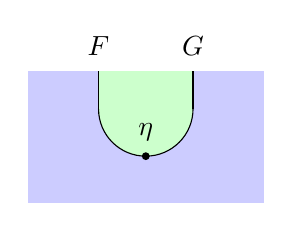
\begin{tikzpicture}[x=0.6cm,y=0.6cm, baseline=(current bounding box.center)]
        \fill[fill=blue!20] (-2.5,0) rectangle (2.5,2.8);
        \filldraw[fill=green!20] (-1,2) arc (180:360:1);
        \fill[fill=green!20] (-1,2) rectangle (1,2.8);
        \node[above=2pt] at (-1,2.8) {$F$};
        \node[above=2pt] at (1,2.8) {$G$};
        \node[above=2pt] at (0,1) {$\eta$};
        \draw[fill=black] (0, 1) circle (0.07);
        \draw (-1,2) -- (-1,2.8);
        \draw (1,2) -- (1,2.8);
    \end{tikzpicture}
\end{center}
defined by $\eta_X:=\varphi_{X,L(X)}(\mathrm{id}_{L(X)})$ for any $X\in \mathrm{Ob}(\mathsf{C})$, where $\varphi_{X,L(X)}$ is the natural bijection
$$
\begin{aligned}
    \varphi_{X,L(X)}:\operatorname{Hom}_{\mathsf{D}}\left(L(X), L(X)\right) & \xlongrightarrow{\sim}\operatorname{Hom}_{\mathsf{C}}(X, RL(X)) \\
\operatorname{id}_{F X} & \longmapsto \eta_X 
\end{aligned}
$$
The \textbf{adjunction counit} $\varepsilon$ of this adjunction is a natural transformation
\begin{center}
    \begin{tikzcd}[ampersand replacement=\&]
        \mathsf{D} \arrow[r, "\scalebox{1.2}{$L\circ R$}"{name=A, above}, bend left=40] \arrow[r, "\scalebox{1.2}{$\mathrm{id}_{\mathsf{D}}$}"'{name=B, below}, bend right=40] 
        \&[+25pt] \mathsf{D}
        \arrow[Rightarrow, shorten <=3.5pt, shorten >=3.5pt, from=A.south-|B, to=B, "\varepsilon"]
    \end{tikzcd}
    \hspace{3cm}
    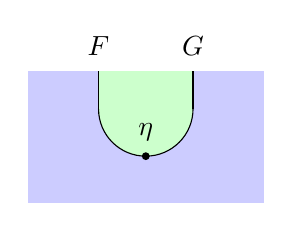
\begin{tikzpicture}[x=0.6cm,y=0.6cm, baseline=(current bounding box.center)]
        \fill[fill=blue!20] (-2.5,0) rectangle (2.5,2.8);
        \filldraw[fill=green!20] (-1,2) arc (180:360:1);
        \fill[fill=green!20] (-1,2) rectangle (1,2.8);
        \node[above=2pt] at (-1,2.8) {$F$};
        \node[above=2pt] at (1,2.8) {$G$};
        \node[above=2pt] at (0,1) {$\eta$};
        \draw[fill=black] (0, 1) circle (0.07);
        \draw (-1,2) -- (-1,2.8);
        \draw (1,2) -- (1,2.8);
    \end{tikzpicture}
\end{center}
}
\pf{
    The naturality square of $\eta$ means that for any morphism $g:X_1\to X_2$ in $\mathsf{C}$, the following diagram commutes
\[
    \begin{tikzcd}[ampersand replacement=\&]
        X_1 \arrow[d, "{\eta_{X_1}}"'] \arrow[r, "g"] \&[+50pt]X_2\arrow[d, "{\eta_{X_2}}"]    \\[+20pt]
         R(L(X_1))\arrow[r, "R(L(g))"']\& R(L(X_2))
    \end{tikzcd}
\] 
}
\section{Monoidal Category}
\dfn{Monoidal Category}{
    A monoidal category is a category $\mathsf{V}$ equipped with
    \begin{enumerate}[(i)]
        \item Tensor product: a functor $\otimes:\mathsf{V}\times\mathsf{V}\to\mathsf{V}$.
        \[
            \begin{tikzcd}[ampersand replacement=\&]
                \mathsf{V}\times \mathsf{V}\&[-25pt]\&[+10pt]\&[-30pt] \mathsf{V}\&[-30pt]\&[-30pt] \\ [-15pt] 
                (X_1,Y_1)  \arrow[dd, "f\times g"{name=L, left}] 
                \&[-25pt] \& [+10pt] 
                \& [-30pt]X_1\otimes Y_1\arrow[dd, "f\otimes g"{name=R}] \\ [-10pt] 
                \&  \phantom{.}\arrow[r, "\otimes", squigarrow]\&\phantom{.}  \&   \\[-10pt] 
                (X_2,Y_2)  \& \& \& X_2\otimes Y_2
            \end{tikzcd}
            \]
        \item Associator: a natural isomorphism $a$
        \[
            \begin{tikzcd}[ampersand replacement=\&]
                \mathsf{V}\times\mathsf{V}\times\mathsf{V} \arrow[r, "(-\otimes-)\otimes-"{name=A, above}, bend left] \arrow[r, "-\otimes(-\otimes-)"'{name=B, below}, bend right] \&[+30pt] \mathsf{V}
                \arrow[Rightarrow, shorten <=5.5pt, shorten >=5.5pt, from=A.south-|B, to=B, "a", "\sim\hspace{1pt}"']
            \end{tikzcd}
        \]
        \item Unit object: an object $1\in \mathrm{Ob}(\mathsf{V})$ 
        \item An isomorphism in $\mathsf{V}$: $\iota:1\otimes 1\to 1$
    \end{enumerate}
    such that the following two condition holds
    \begin{enumerate}[(i)]
        \item The pentagon axiom: the following diagram commutes
    \[
        \begin{tikzcd}[ampersand replacement=\&, column sep=small]
            \& [-50pt]                  \&[-25pt]    ((A\otimes B)\otimes C)\otimes D \arrow[lld, "{a_{(A,B,C)}\otimes \mathrm{id}_D}"'] \arrow[rrd, "{a_{(A\otimes B,C,D)}}"] \& [-25pt]                  \&   [-50pt]                                                                      \\[+20pt]
(A\otimes( B\otimes C))\otimes D \arrow[rd, "{a_{(A,B\otimes C,D)}}"'] \&                                                                                    \&    \&       \& (A\otimes B)\otimes (C\otimes D) \arrow[ld, "{a_{(A, B, C\otimes D)}}"] \\[+35pt]
            \& A\otimes( (B\otimes C)\otimes D) \arrow[rr, "{\mathrm{id}_A\otimes a_{(B,C,D)}}"'] \&    \& A\otimes( B\otimes (C\otimes D)) \&                                                                        
\end{tikzcd}
    \]
    \item Unit axiom: the functors $1\otimes -:\mathsf{V}\to\mathsf{V}$ and $-\otimes 1:\mathsf{V}\to\mathsf{V}$ are category equivalences.
    \end{enumerate}
}

A strict monoidal category is one for which the natural isomorphisms $a$, $\lambda$ and $\rho$ are identities. Every monoidal category is monoidally equivalent to a strict monoidal category.

\dfn{Cartesian/Cocartesian Monoidal Category}{
    \begin{itemize}[leftmargin=8pt]
        \item A \textbf{cartesian monoidal category} is a monoidal category where the tensor product is the categorical product and the unit object is the terminal object. 
        \item A \textbf{cocartesian monoidal category} is a monoidal category where the tensor product is the categorical coproduct and the unit object is the initial object.
    \end{itemize}
}
\ex{Category of Endofunctors is a Monoidal Category}{
    Let $\mathsf{C}$ be a category. The \textbf{category of endofunctors} $\left[\mathsf{C},\mathsf{C}\right]$ is a monoidal category with the following structure
    \begin{enumerate}[(i)]
        \item Tensor product: composition of functors.
        \item Associator: the natural isomorphism $a$ is the identity.
        \item Unit object: the identity functor $\mathrm{id}_{\mathsf{C}}$.
        \item Unit isomorphism: the natural isomorphism $\iota$ is the identity.
    \end{enumerate}
}

\section{Enriched Category}
\dfn{Enriched Category}{
    Let $\mathsf{V}$ be a monoidal category. An \textbf{$\mathsf{V}$-enriched category} $\mathsf{C}$ consists of
    \begin{enumerate}[(i)]
        \item Object set: a set of objects $\mathrm{Ob}(\mathsf{C})$.
        \item $\mathrm{Hom}$-object: for each pair of objects $A,B\in \mathrm{Ob}(\mathsf{C})$, an object $\mathrm{Hom}_{\mathsf{C}}(A,B)\in \mathrm{Ob}(\mathsf{V})$.
        \item Composition: for each triple of objects $A,B,C\in \mathrm{Ob}(\mathsf{C})$, a morphism in $\mathsf{V}$
        \[
            \circ:\mathrm{Hom}_{\mathsf{C}}(B,C)\otimes \mathrm{Hom}_{\mathsf{C}}(A,B)\longrightarrow \mathrm{Hom}_{\mathsf{C}}(A,C)
        \]
        \item Identity: for each object $A\in \mathrm{Ob}(\mathsf{C})$, a morphism ${\mathcal{I}d}_A:1 \to \mathrm{Hom}_{\mathsf{C}}(A,A)$ in $\mathsf{V}$.
    \end{enumerate}
    such that the following conditions hold
    \begin{enumerate}[(i)]
        \item For each quadruple of objects $A,B,C,D\in \mathrm{Ob}(\mathsf{C})$, the following diagram in $\mathsf{V}$ commutes
        \[
            \begin{tikzcd}[ampersand replacement=\&, column sep=small]
                    \&[-130pt] {\left(\mathrm{Hom}(C,D)\otimes \mathrm{Hom}(B,C)\right)\otimes \mathrm{Hom}(A,B) } \arrow[ld, "\circ\;\otimes \,\mathrm{id}_{\mathrm{Hom}(A,B)}"'] \arrow[rr, "\cong"] \&  [-30pt]   \&  [-30pt]{\mathrm{Hom}(C,D)\otimes \left(\mathrm{Hom}(B,C)\otimes \mathrm{Hom}(A,B)\right) } \arrow[rd, "\mathrm{id}_{\mathrm{Hom}(C,D)}\,\otimes\;\circ "] \&  [-130pt]  \\[+35pt]
{\mathrm{Hom}(B,D)\otimes \mathrm{Hom}(A,B) } \arrow[rrd, "\circ"'] \&                                                                                                                                    \&                                               \&                                                                                                               \& {\mathrm{Hom}(C,D)\otimes \mathrm{Hom}(A,C) } \arrow[lld, "\circ"] \\[+20pt]
                    \&                                                                                                                                    \& {\mathrm{Hom}(A,D)} \&                                                                                                               \&                                                                   
\end{tikzcd}
    \]
    \item For each pair of objects $A,B\in \mathrm{Ob}(\mathsf{C})$, the following diagrams in $\mathsf{V}$ commute
    \[
    \begin{tikzcd}[ampersand replacement=\&, column sep=small]
        {1\otimes \mathrm{Hom}_{\mathsf{C}}(A,B)} \arrow[rr, "{{\mathcal{I}d}_B\otimes\,\mathrm{id}_{\mathrm{Hom}_{\mathsf{C}}(A,B)}}"] \arrow[rd, "\cong"'] \&                     \& {\mathrm{Hom}_{\mathsf{C}}(B,B)\otimes \mathrm{Hom}_{\mathsf{C}}(A,B)} \arrow[ld, "\circ"] \\[+10pt]
        \& {\mathrm{Hom}_{\mathsf{C}}(A,B)} \&   
\end{tikzcd}
    \]
    \[
        \begin{tikzcd}[ampersand replacement=\&, column sep=small]
            {\mathrm{Hom}_{\mathsf{C}}(A,B)\otimes 1} \arrow[rr, "\mathrm{id}_{\mathrm{Hom}_{\mathsf{C}}(A,B)}\otimes\,{\mathcal{I}d}_A "] \arrow[rd, "\cong"'] \&                     \& {\mathrm{Hom}_{\mathsf{C}}(A,B)\otimes \mathrm{Hom}_{\mathsf{C}}(A,A)} \arrow[ld, "\circ"] \\[+10pt]
            \& {\mathrm{Hom}_{\mathsf{C}}(A,B)} \&
    \end{tikzcd}
        \]
    \end{enumerate}
}


\section{Abelian Category}
Some literature refers to $\mathsf{Ab}$-categories as preadditive categories. We will not use this term in this note.



\dfn{Biproduct}{
    Let $\mathsf{C}$ be an $\mathsf{Ab}$-category and $X_1$, $X_2$ be objects in $\mathsf{C}$. A \textbf{biproduct} of $X_1$ and $X_2$ is a diagram
    \[
    \begin{tikzcd}[ampersand replacement=\&]
            X_1 \arrow[r, "i_1", shift left] \& X_1\oplus X_2 \arrow[l, "p_1", shift left] \arrow[r, "p_2"', shift right] \& X_2 \arrow[l, "i_2"', shift right]
    \end{tikzcd}
    \]
    such that
    \begin{itemize}
        \item $p_1\circ i_1=\mathrm{id}_{X_1}$, $p_2\circ i_2=\mathrm{id}_{X_2}$.
        \item $i_1\circ p_1+ i_2\circ p_2=\mathrm{id}_{X_1\oplus X_2}$.
    \end{itemize}
    Empty biproduct is defined to be the zero object.
}

\prop{Equivalent Conditions of Existance of Biproduct}{
    Let $\mathsf{C}$ be an $\mathsf{Ab}$-category and $X_1$, $X_2$ be objects in $\mathsf{C}$. Then the following are equivalent
    \begin{enumerate}[(i)]
        \item Product $X_1\times X_2$ exists.
        \item Coproduct $X_1\amalg X_2$ exists.
        \item Biproduct $X_1\oplus X_2$ exists.
    \end{enumerate}
}
\prop{Equivalent Conditions of Existance of Zero Object}{
    Let $\mathsf{C}$ be an $\mathsf{Ab}$-category. Then the following are equivalent
    \begin{enumerate}[(i)]
        \item Initial object (empty product) exists.
        \item Terminal object (empty coproduct) exists.
        \item Zero object (empty biproduct) exists.
    \end{enumerate}
}
\prop{$\mathsf{Ab}$-enriched functors preserve biproducts}{
    $\mathsf{Ab}$-enriched functors preserve finite biproducts.
}
\dfn{Additive Category}{
    An $\mathsf{Ab}$-category is \textbf{additive} if it has all finite biproducts.
}

\dfn{Kernel and Cokernel}{
    Suppose $\mathsf{C}$ is an abelian category with zero object and $f:X\to Y$ is a morphism in $\mathsf{C}$. The \textbf{kernel} of $f$ is the equalizer of $f$ and the zero morphism, which is denoted by $\ker f$. The universal property of kernel is given by the following diagram
    \[
    \begin{tikzcd}[ampersand replacement=\&]
        \& M \arrow[d, "g"] \arrow[rd, "0"] \arrow[ld, "\exists!\widetilde{g}"', dashed] \&   \\
        \ker f \arrow[r] \& X \arrow[r, "f"']                                                             \& Y
    \end{tikzcd}
    \]
    The \textbf{cokernel} of $f$ is the coequalizer of $f$ and the zero morphism, which is denoted by $\operatorname{coker}f$. The universal property of cokernel is given by the following diagram
    \[
    \begin{tikzcd}[ampersand replacement=\&]
        \& M                           \&                                                                     \\
        X \arrow[r, "f"'] \arrow[ru, "0"] \& Y \arrow[u, "g"'] \arrow[r] \& \operatorname{coker} f \arrow[lu, "\exists!\widetilde{g}"', dashed]
        \end{tikzcd}
    \]

}

\dfn{Abelian Category}{
    An additive category $\mathsf{C}$ is \textbf{abelian} if 
    \begin{enumerate}[(i)]
        \item Every morphism has both a kernel and a cokernel.
        \item Every monomorphism and every epimorphism is normal. This means that every monomorphism is a kernel of some morphism, and every epimorphism is a cokernel of some morphism.
    \end{enumerate}
}

\prop{}{
    If $\mathsf{A}$ is an abelian category, then $\left[\mathsf{C}^\mathrm{op}, \mathsf{A}\right]$ is abelian for any small category $\mathsf{C}$.
}


\chapter{Group}
\section{Basic Concepts}
\dfn{Group}{
    A \textbf{group} is a set $G$ together with a binary operation $\cdot:G\times G\to G$ such that
    \begin{enumerate}[(i)]
        \item (Associativity) $\forall x,y,z\in G$, $(x\cdot y)\cdot z=x\cdot(y\cdot z)$.
        \item (Identity) $\exists e\in G$ such that $\forall x\in G$, $e\cdot x=x\cdot e=x$.
        \item (Inverse) $\forall x\in G$, $\exists x^{-1}\in G$ such that $x\cdot x^{-1}=x^{-1}\cdot x=e$.
    \end{enumerate}
}
Since the identity of a group is unique, we denote it by $1_G$ or simply $1$.
\dfn{Opposite Group}{
    Let $G=(G,*)$ be a group. The \textbf{opposite group} of $G$ is the group $G^{\mathrm{op}}=(G,*^{\mathrm{op}})$, where $*^{\mathrm{op}}:G\times G\to G$ is defined by $x*^{\mathrm{op}}y=y\cdot x$. If we consider $G$ as a category $\mathsf{B}G$, then we have category isomorphism
    \[
        \mathsf{B}G^{\mathrm{op}}\cong (\mathsf{B}G)^{\mathrm{op}}.
    \]
}
\dfn{Subgroup}{
    Let $G$ be a group. A subset $H$ of $G$ is called a \textbf{subgroup} of $G$ if $H$ is a group with respect to the binary operation of $G$. In this case, we write $H\le G$.
}


\section{Group Homomorphism}
\dfn{Group Homomorphism}{
    Let $G,H$ be groups. A \textbf{group homomorphism} from $G$ to $H$ is a function $\varphi:G\to H$ such that
    \[
        \forall x,y\in G,\quad \varphi(x y)=\varphi(x)\varphi(y).
    \]
}
\dfn{Isomorphism}{
    Let $G,H$ be groups. A group homomorphism $\varphi:G\to H$ is called an \textbf{isomorphism} if $\varphi$ is bijective. In this case, we say that $G$ and $H$ are \textbf{isomorphic} and write $G\cong H$.
}
\prop{Properties of Group Homomorphisms}{
    Let $G,H$ be groups and $\varphi:G\to H$ be a group homomorphism. Then
    \begin{enumerate}[(i)]
        \item $\varphi(1_G)=1_H$.
        \item $\forall x\in G$, $\varphi(x^{-1})=\varphi(x)^{-1}$.
        \item $\forall n\in\mathbb{Z}$, $\varphi(x^n)=\varphi(x)^n$.
        \item If $K\le G$ , then $\varphi(K)\le H$.
        \item If $K\le H$, then $\varphi^{-1}(K)\le G$.
    \end{enumerate}
}
\dfn{Kernel of Group Homomorphism}{
    Let $\varphi:G\to H$ be a group homomorphism. The \textbf{kernel} of $\varphi$ is defined by
    \[
        \ker\varphi=\{x\in G\mid \varphi(x)=1_H\}.
    \]
}
\prop{Property of Kernel}{
    Let $G$ be a group. Then
    \begin{enumerate}[(i)]
        \item Let $\varphi:G\to H$ be a group homomorphism. Then $\varphi$ is injective if and only if $\ker\varphi=\{1_G\}$.
    \end{enumerate}
}
\dfn{Normal Subgroup}{
    Let $G$ be a group. A subgroup $H$ of $G$ is called a \textbf{normal subgroup} if $gHg^{-1}=H$ for all $g\in G$. In this case, we write $H\lhd G$.
}
\prop{Equivalent Definition of Normal Subgroup}{
    Let $G$ be a group and $H$ be a subgroup of $G$. Then the following are equivalent:
    \begin{enumerate}[(i)]
        \item $H$ is a normal subgroup of $G$.
        \item $\forall \gamma_g \in\mathrm{Inn}(G)$, $\gamma_g(H)\subseteq H$.
        \item $gHg^{-1}\subseteq H$ for all $g\in G$.
        \item $gHg^{-1}=H$ for all $g\in G$.
        \item $gH=Hg$ for all $g\in G$.
        \item $H$ is a union of conjugacy classes.
        \item $H=\ker\varphi$ for some group homomorphism $\varphi:G\to K$.
    \end{enumerate}
}
\prop{Properties of Normal Subgroup}{
    Let $G$ be a group.
    \begin{enumerate}[(i)]
        \item $\{1_G\}$ and $G$ are normal subgroups of $G$.
        \item If $H\le K\le G$ and $H\lhd G$, then $H\lhd K$.
        \item If $H\lhd_{\rm char} K\lhd G$, then $H\lhd G$.
        \item Normality is preserved under surjective homomorphisms: if $f:G \rightarrow H$ is a surjective group homomorphism and $N\lhd G$, then $f(N)\lhd H$.
        \item Normality is preserved by taking inverse images of homomorphisms: if $f:G \rightarrow H$ is a group homomorphism and $N\lhd H$, then $f^{-1}(N)\lhd G$.
        \item Normality is preserved on taking finite products: if $N_1 \lhd G_1$ and $N_2 \lhd G_2$, then $N_1 \times N_2 \lhd G_1 \times G_2$.
        \item Given two normal subgroups, $N$ and $M$, of $G$, their intersection $N \cap M$ and their product $N M=\{n m: n \in N$ and $m \in M\}$ are also normal subgroups of $G$.
    \end{enumerate}
}
\dfn{Simple Group}{
    A group $G$ is called \textbf{simple} if $G$ is nontrivial and the only normal subgroups of $G$ are $\{1_G\}$ and $G$.
}
\thm{Fundamental Theorem on Homomorphisms}{
    Let $G,H$ be groups and $\varphi:G\to H$ be a group homomorphism. Define natural projection 
    \begin{align*}
        \pi:G&\longrightarrow G/\ker\varphi\\
        g&\longmapsto g\ker\varphi
    \end{align*}
    Then there exists a unique group homomorphism $\overline{\varphi}:G/\ker\varphi\to H$ such that the following diagram commutes
    \begin{center}
        \begin{tikzcd}[ampersand replacement=\&]
            G \arrow[r, "\varphi"] \arrow[d, "\pi"'] \& H \\[0.3cm]
            G/\ker\varphi \arrow[ru, dashed, "\exists!\,\overline{\varphi}"'] \&  
        \end{tikzcd}
    \end{center}
    Moreover, $\overline{\varphi}$ is injective and we have $ G/\ker\varphi\cong \mathrm{im}\varphi$.
}
\cor{First isomorphism theorem}{
    Let $G,H$ be groups and $\varphi:G\to H$ be surjective group homomorphism. Then $G/\ker\varphi\cong H$.
}

\prop{Universal Property of Quotient Group}{
    Let $G$ be a group and $N \lhd G$ be a normal subgroup. Suppose $\pi:G\to G/N$ is the natural projection. Then $\pi$ is initial in the category of group homomorphisms $\varphi:G\to H$ such that $N\subseteq \ker\varphi$. \\
    That is, for any group $H$ and group homomorphism $\varphi:G\to H$ such that $N\subseteq \ker\varphi$, there exists a unique group homomorphism $\widetilde{\varphi}:G/N\to H$ such that the following diagram commutes
    \begin{center}
        \begin{tikzcd}[ampersand replacement=\&]
            G \arrow[r, "\varphi"] \arrow[d, "\pi"'] \& H \\[0.3cm]
            G/N \arrow[ru, dashed, "\exists !\,\widetilde{\varphi}"'] \&  
        \end{tikzcd}
    \end{center}
}
\proof{
    Since $N\subseteq \ker\varphi$, there is a canonical projection 
    \begin{align*}
        p:G/N &\longrightarrow G/\ker\varphi\\
        gN &\longmapsto g\ker\varphi
    \end{align*}
    According to the following diagram, we can define $\widetilde{\varphi}$ by $\widetilde{\varphi}=\overline{\varphi}\circ p$.
    \begin{center}
        \begin{tikzcd}[ampersand replacement=\&]
            G \arrow[r, "\varphi"] \arrow[d, "\pi"'] \& H \\[0.4cm]
            G/N \arrow[ru, dashed, "\widetilde{\varphi}"'] \arrow[r,"p"'] \&  G/\ker\varphi \arrow[u, dashed, "\overline{\varphi}"']
        \end{tikzcd}
    \end{center}
}
\thm{Second Isoomorphism Theorem}{
    Let $G$ be a group and $H,K$ be subgroups of $G$. Then $HK$ is a subgroup of $G$ and $H\cap K$ is a normal subgroup of $H$. Moreover, we have
    \[
        HK/H\cong K/(H\cap K).
    \]
}
\section{Construction}
\subsection{Free Object}
Let $A$ be set. Define a \textbf{string} over the $A$ to be a finite sequence of elements of $A$. The \textbf{concatenation} of two strings $\overline{a_1\cdots a_n}$ and $\overline{b_1\cdots b_m}$ is a binary operation $\diamond$ defined by
\[
    \overline{a_1\cdots a_n}\diamond \overline{b_1\cdots b_m}=\overline{a_1\cdots a_nb_1\cdots b_m}.
\]
\dfn{Word}{
    Let $S$ be a set. Define $S^{-1}=\left\{s^{-1}\midv s\in S\right\}$. A \textbf{word} on $S$ is a string over $S\sqcup S^{-1}\sqcup\{1\}$. $\overline{1}$ is called an \textbf{empty word}. The \textbf{length} of a word $w$ is the number of letters in $w$.
}
\dfn{Reduced Word}{
    Let $W(S)$ be the set of all words on $S$. Define a relation $\approx$ on $W(S)$ as follows: for any $s\in S$
    \begin{align*}
        \overline{s^{-1}s}\approx \overline{1},\quad \overline{ss^{-1}}\approx \overline{1}, \quad \overline{1s}\approx s,\quad \overline{s1}\approx \overline{1}
    \end{align*}
    Define $\sim$ to be the equivalence relation generated by $\approx$. Let $\pi:W(S)\to W(S)/\sim, w\mapsto [w]_\sim$ denote the quotient map. It is easy to see that for any $[w]_\sim\in W(S)/\sim$, there exists a unique representative element $\rho(w)\in W(S)$ which has shortest length among all representatives of $[w]_\sim$. A word $w$ is called \textbf{reduced} if $\rho(w)=w$. 
}

\dfn{Free Group}{
    Let $S$ be a set. The \textbf{free group} on $S$, denoted by $\mathrm{Free}_{\mathsf{Grp}}(S)$, together with a function $\iota:S\to \mathrm{Free}_{\mathsf{Grp}}(S)$, is defined by the following universal property: for any group $G$ and any function $f:S\to G$, there exists a unique group homomorphism $\widetilde{f}:\mathrm{Free}_{\mathsf{Grp}}(S)\to G$ such that the following diagram commutes
    \begin{center}
        \begin{tikzcd}[ampersand replacement=\&]
            \mathrm{Free}_{\mathsf{Grp}}(S)\arrow[r, dashed, "\exists !\,\widetilde{f}"]  \& G \\[0.3cm]
            S\arrow[u, "\iota"] \arrow[ru, "f"'] \&  
        \end{tikzcd}
    \end{center}
    The free group $\mathrm{Free}_{\mathsf{Grp}}(S)$ can be contructed as follows: as a set it consists of all reduced words on $S$. The binary operation $\cdot$ is concatenation with reduction defined by
    \[
    w_1\cdot w_2 = \rho(w_1\diamond w_2).    
    \]
    The identity element is the empty word. The inverse of a word is obtained by reversing the order of the letters and replacing each letter by its inverse.
}

\prop{Free-Forgetful Adjunction}{
    The free group functor $\mathrm{Free}_{\mathsf{Grp}}$ is left adjoint to the forgetful functor $U:\mathsf{Grp}\to \mathsf{Set}$
    $$
    \begin{tikzcd}[ampersand replacement=\&]
        \mathsf{Set} \arrow[rr, "\mathrm{Free}_{\mathsf{Grp}}", bend left] \&[-10pt]\bot\&[-10pt] \mathsf{Grp} \arrow[ll, "U", bend left]
        \end{tikzcd}
        $$
    The adjunction isomorphism is given by
    \begin{align*}
        \varphi_{S,G}:\mathrm{Hom}_{\mathsf{Grp}}(\mathrm{Free}_{\mathsf{Grp}}(S),G)&\xlongrightarrow{\sim} \mathrm{Hom}_{\mathsf{Set}}(S,U(G))\\
        g&\longmapsto g\circ \iota
    \end{align*}
}
\pf{
    First we show that $\varphi_{S,G}$ is injective. Suppose $g_1,g_2:\mathrm{Free}_{\mathsf{Grp}}(S)\to G$ are two group homomorphisms such that $g_1\circ \iota=g_2\circ \iota$. By the universal property of free group, we have $g_1=g_2$. Then we show that $\varphi_{S,G}$ is surjective. Suppose $f:S\to U(G)$ is a function. By the universal property there exists a group homomorphism $\widetilde{f}:\mathrm{Free}_{\mathsf{Grp}}(S)\to G$ such that $\varphi_{S,G}(\widetilde{f})=\widetilde{f}\circ \iota=f$. Finally, we show that $\varphi_{S,G}$ is natural in $S$ and $G$. Suppose $h:S_1\to S_2$ is a function and $q:G_1\to G_2$ is a group homomorphism. Then we can check that for any $g\in \mathrm{Hom}_{\mathsf{Grp}}(\mathrm{Free}_{\mathsf{Grp}}(S_2),G_2)$,
    \begin{align*}
        \varphi_{S_1,G_1}(q\circ g\circ \iota_{S_1})&=(q\circ g\circ \iota_{S_1})\circ \iota_{S_1}\\
        &=q\circ g\circ (\iota_{S_1}\circ \iota_{S_1})\\
        &=q\circ g\circ \iota_{S_2}\\
        &=\varphi_{S_2,G_2}(g\circ \iota_{S_2}).
    \end{align*}

}

\subsection{Inverse Limit}
\dfn[inverse_limit_of_groups]{Inverse Limit in $\mathsf{Grp}$}{
    Let $\mathsf{I}$ be a \hyperref[th:filtered_category]{filtered} \hyperref[th:thin_category]{thin category} and $F:\mathsf{I}^{\mathrm{op}}\to \mathsf{Grp}$ be a functor. To unpack the information of $F$, denote $I:=\mathrm{Ob}(\mathsf{I})$, $G_i:=F(i)$ and $f_{ij}:=F(i\to j)$. An \textbf{inverse system} is a pair $\left(\left(G_i\right)_{i \in I},\left(f_{i j}\right)_{i \leq j \in I}\right)$ where $f_{i j}: G_{j} \rightarrow G_{i}$ is a group homomorphism for each $i \leq j$ such that
    \begin{enumerate}[(i)]
        \item $f_{i i}=\mathrm{id}_{G_i}$ for all $i \in I$.
        \item $f_{i k}=f_{i j} \circ f_{j k}$ for all $i \leq j \leq k$.
    \end{enumerate}
    The \textbf{inverse limit} of $\left(\left(G_i\right)_{i \in I},\left(f_{i j}\right)_{i \leq j \in I}\right)$ is the cofiltered limit $\varprojlim F$, also denoted by $\varprojlim_{i\in I}G_i$, which can be constructed as a subgroup of $\prod_{i \in I} G_{i}$ as follows
    \[
        \varprojlim_{i\in I}G_i \cong \left\{(x_i)_{i\in I}\in \prod_{i \in I} G_{i}\midv x_i=f_{ij}(x_j) \text{ for all }i\le j \in I\right\}
    \]
    equipped with natural projections $\pi_i:\varprojlim_{i\in I}G_i\to G_i$.\\

}

\ex{Inverse Limit $\varprojlim_{i\ge 1}G_i$}{
    Let $\mathsf{I}=\left(\mathbb{Z}_{\ge 1},\le\right)$ be a filtered thin category and $F:\mathsf{I}^{\mathrm{op}}\to \mathsf{Grp}$ be a functor. To determine an inverse system, it is sufficient to specify $G_i$ and $f_{i,i+1}:G_{i+1}\to G_i$ for all $i\in \mathbb{Z}_{\ge 1}$. The inverse limit of this inverse system is denoted by $\varprojlim_{i\ge 1}G_i$, which we now write as $G$ for simplicity.\\
    $G$ can be imaged as a tree with root layer being $G_0=\{1\}$ and $i$-th layer being $G_i$. Each node in $G_i$ has a unique parent node in $G_{i-1}$, which is determined by $f_{i,i-1}$. An element in $G$ is a path starting from the root and passing through each $G_i$ exactly once along the edges of the tree. The $i$-th component $x_i$ of an element $x\in G$ includes all information of its history path from $G_0$ to $G_i$, which makes $x_1,x_2,\cdots, x_{i-1}$ redundant. 
}

\section{Group Action}
\subsection{Definitions}
\dfn{Symmetric Group}{
    The \textbf{symmetric group} on a set $X$ is the group whose elements are all bijections from $X$ to $X$, with the group operation of function composition. The symmetric group on $X$ is denoted by $\mathrm{Sym}(X)$ or $\mathrm{Aut}_{\mathsf{Set}}(X)$. If $X=\{1,2,\cdots,n\}$, then we denote $\mathrm{Sym}(X)$ by $S_n$.
}
\dfn{Group Action}{
    Let $G$ be a group and $X$ be a set. A \textbf{group action} of $G$ on $X$ is a group homomorphism
    \begin{align*}
        \sigma:G&\longrightarrow \mathrm{Aut}_{\mathsf{Set}}(X)\\
        g&\longmapsto \sigma_g
    \end{align*}
    If $G$ acts on $X$ by $\sigma$, we say $(X,\sigma)$ is a \textbf{$G$-set}. If there is no ambiguity, we simply say $X$ is a $G$-set.
}
The $G$-sets and $G$-maps form a category $G\text{-}\mathsf{Set}$ and we have category isomorphism
\begin{align*}
    G\text{-}\mathsf{Set}&\stackrel{\sim}{\longrightarrow}[\mathsf{B}G, \mathsf{Set}]    \\
    \sigma&\longmapsto \sigma(-)
\end{align*}
\prop{Equivalent Definition of Group Actions}{
    Let $G$ be a group and $X$ be a set. A group action of $G$ on $X$ can be alternatively defined as a map
    \begin{align*}
        \cdot:G\times X&\longrightarrow X\\
        (g,x)&\longmapsto g\cdot x
    \end{align*}
    such that
    \begin{enumerate}[(i)]
        \item $\forall x\in X$, $e\cdot x=x$.
        \item $\forall g,h\in G$, $\forall x\in X$, $(gh)\cdot x=g\cdot(h\cdot x)$.
    \end{enumerate}
    The equivalence of the two definitions is given by
    \[
    \sigma_g(x)=g\cdot x.
    \]
}
We say $X$ is a right $G$-set if $X$ is a left $G^{\mathrm{op}}$-set.
\ex{Trivial Group Action}{
    Let $G$ be a group and $X$ be a set. The \textbf{trivial group action} of $G$ on $X$ is defined as $\sigma_g=\mathrm{id}_X$ for all $g\in G$.
}
\ex[acting_on_power_set]{Actions on $X$ Induce Actions on $2^X$}{
    If a group $G$ acts on a set $X$, then $G$ acts on the power set $2^X$ by
    \[
    g\cdot A=\{ g\cdot x\mid x\in A\}    .
    \]
}
\dfn{Equivariant Map}{
    Let $G$ be a group and $X,Y$ be $G$-sets. A map $f:X\to Y$ is called \textbf{equivariant} if for all $g\in G$ and $x\in X$, we have
    \[
    f(g\cdot x)=g\cdot f(x)    .
    \]
    Equivalently, $f$ is equivariant if it is a natural transformation $f:\sigma(-)\implies \sigma'(-)$
    \[
        \begin{tikzcd}[ampersand replacement=\&, column sep=1.7em, row sep=small]
            \mathsf{B}G  \& \bullet \arrow[rr, "g"]                         \&  \& \bullet                 \\
                         \& X \arrow[dd, "f"'] \arrow[rr, "\sigma_g"] \&  \& X \arrow[dd, "f"] \\
            \mathsf{Set} \&                                           \&  \&                   \\
                         \& Y \arrow[rr, "\sigma'_g"']                \&  \& Y                
            \end{tikzcd}
    \]
}
\dfn{Product of $G$-Sets}{
    The \textbf{product} of two $G$-sets $X$ and $Y$ is defined as the set $X\times Y$ with the $G$-action
    \[
    g\cdot (x,y)=(g\cdot x, g\cdot y)    .
    \]
    Alternatively, the product of two $G$-sets can be defined as the product of two functors, cf. \Cref{th:ev_functor_preserves_limits}.
}
\dfn{Coproduct of $G$-Sets}{
    The \textbf{coproduct} of two $G$-sets $X$ and $Y$ is defined as the set $X\sqcup Y$ with the $G$-action
    \[
    g\cdot a=\begin{cases}
        g\cdot a & a\in X\\
        g\cdot a & a\in Y
    \end{cases} 
    \]
    Alternatively, the coproduct of two $G$-sets can be defined as the coproduct of two functors, cf. \Cref{th:ev_functor_preserves_limits}.
}
\ex[aut_acts_on_hom]{$\mathrm{Aut}_\mathsf{C}(X)$ acts on $\mathrm{Hom}_\mathsf{C}(X,Y)$ and $\mathrm{Hom}_\mathsf{C}(Y,X)$}{
    Let $X$ and $Y$ be objects in a category $\mathsf{C}$. Then $\mathrm{Aut}_\mathsf{C}(X)$ acts on $\mathrm{Hom}_\mathsf{C}(X,Y)$ by the composition of functors
    \[
    \begin{tikzcd}[ampersand replacement=\&, column sep=5em, row sep=3em]
    \mathsf{B}\mathrm{Aut}_\mathsf{C}(X)\arrow[r] \&[-3em] \mathsf{B}\mathrm{Aut}_\mathsf{C}(X)^{\mathrm{op}} \arrow[r, hook] \&[-2em] \mathsf{C}^{\mathrm{op}} \arrow[r, "{\mathrm{Hom}_{\mathsf{C}}(-,Y)}"] \& \mathsf{Set}\\[-2.3em]
    \bullet \arrow[r, maps to] \arrow[d, "g"']           \& \bullet \arrow[r, maps to] \arrow[d, "g^{-1}"]                           \& X \arrow[d, "g^{-1}"] \arrow[r, maps to]                               \& {\mathrm{Hom}(X,Y)} \arrow[d, "\left(g^{-1}\right)^*"] \\
    \bullet \arrow[r, maps to]                           \& \bullet \arrow[r, maps to]                                               \& X \arrow[r, maps to]                                                   \& {\mathrm{Hom}(X,Y)}  
    \end{tikzcd}
    \]
    Writing explicily, the action is given by
    \begin{align*}
        \mathrm{Aut}_\mathsf{C}(X)\times \mathrm{Hom}_\mathsf{C}(X,Y)&\longrightarrow \mathrm{Hom}_\mathsf{C}(X,Y)\\
        (g,f)&\longmapsto f\circ g^{-1}
    \end{align*}
    Similarly, $\mathrm{Aut}_\mathsf{C}(Y)$ acts on $\mathrm{Hom}_\mathsf{C}(Y,X)$ by
    \[
    \begin{tikzcd}[ampersand replacement=\&, column sep=5em, row sep=3em]
    \mathsf{B}\mathrm{Aut}_\mathsf{C}(X)\arrow[r, hook] \&[-1em] \mathsf{C} \arrow[r, "{\mathrm{Hom}_{\mathsf{C}}(Y,-)}"] \& \mathsf{Set}\\[-2.3em]
    \bullet \arrow[r, maps to] \arrow[d, "g"']           \&  X \arrow[d, "g"] \arrow[r, maps to]                               \& {\mathrm{Hom}(Y,X)} \arrow[d, "g_*"] \\
    \bullet \arrow[r, maps to]                           \& X \arrow[r, maps to]                                                   \& {\mathrm{Hom}(X,Y)}  
    \end{tikzcd}
    \]
    Writing explicily, the action is given by
    \begin{align*}
        \mathrm{Aut}_\mathsf{C}(Y)\times \mathrm{Hom}_\mathsf{C}(Y,X)&\longrightarrow \mathrm{Hom}_\mathsf{C}(Y,X)\\
        (g,f)&\longmapsto g\circ f
    \end{align*}
}
\ex[acting_on_functions]{Actions on $X$ Induce Actions on $Y^X$}{
    If $G$ acts on $X$ through a functor $\sigma(-):\mathsf{B}G\to\mathsf{Set}$, then it also acts on $Y^X$ for any set $Y$ by the composition of functors 
    \[
    \begin{tikzcd}[ampersand replacement=\&, column sep=5em, row sep=3em]
        \mathsf{B}G \arrow[r] \&[-2em] \mathsf{B}G^{\mathrm{op}} \arrow[r, "\sigma(-)^{\mathrm{op}}"] \&[-2.2em] \mathsf{Set}^{\mathrm{op}} \arrow[r, "{\mathrm{Hom}_{\mathsf{Set}}(-,Y)}"] \& \mathsf{Set}
        \end{tikzcd}
    \]
    The action on $Y^X$ is given explicitly as follows: for all $g\in G$, $f\in Y^X$ and $x\in X$,
    \[
        (g\cdot f)(x)=f(g^{-1}\cdot x).
    \]
    
}
\pf{
    We can check that
    \begin{align*}
        (g_1\cdot (g_2\cdot f))(x)&=\left(g_2\cdot f\right)\left(g_1^{-1}\cdot x\right)\\
        &=\left(g_2\cdot f\right)\left(g_1^{-1}\cdot x\right)\\
        &=f\left(g_2^{-1}\cdot\left(g_1^{-1}\cdot x\right)\right)\\
        &=f\left(\left(g_2^{-1} g_1^{-1}\right)\cdot x\right)\\
        &=\left(\left(g_1g_2\right)\cdot f\right)(x).
    \end{align*}
}
\dfn{Orbit of a Group Action}{
    Let $G$ be a group acting on a set $X$. For $x\in X$, the \textbf{orbit} of $x$ is defined as 
    \[
    G x=\{ g\cdot x\mid g\in G\}    .
    \]
}

\dfn{Orbit Space}{
    Let $G$ be a group acting on a set $X$. The \textbf{orbit space} of $G$ acting on $X$ is defined as 
    \[
    X/G=\{ Gx\mid x\in X\}.
    \]
}
If $G$ acts on $X$, then $G$ acts on $X/G$ trivially.
\prop{Orbit Decomposition}{
    Let $G$ be a group acting on a set $X$. We define a equivalence relation $\sim$ on $X$ by
    \[
    x\sim y \iff Gx=Gy.
    \]
    Then the equivalence class of $x$ is exactly $Gx$. The quotient set $X/\sim$ is exactly the orbit space $X/G$.
    And we have a partition of $X$ by the orbits of $G$ acting on $X$
    \[
    X=\bigsqcup_{Gx\in X/G}Gx.
    \]
}
\pf{
We can check that the equivalence class of $x$ is $Gx$. If $y\sim x$, then $y\in Gy=Gx$. If $y\in Gx$, then $Gy\subseteq Gx$ and $x\in Gy$. Note $x\in Gy$ implies $Gx\subseteq Gy$. We have $Gx=Gy$, i.e. $x\sim y$. 
}

If $G$ acts on $X$, then $G$ acts on $X/G$ trivially.
\dfn{$G$-invariant element }{
    Let $G$ be a group acting on a set $X$. An element $x\in X$ is called \textbf{$G$-invariant} if $Gx=\{ x\}$. The set of all $G$-invariant elements is denoted by $X^G$
    \[
      X^G=\{ x\in X\mid Gx=\{ x\} \}  .  
    \]
}

\dfn{Stabilizer Subgroup}{
    Let $G$ be a group acting on a set $X$. For $x\in X$, the \textbf{stabilizer subgroup} of of $G$ with respect to $x$ is defined as 
    \[
    \mathrm{Stab}_G(x)=\{ g\in G\mid g\cdot x=x\}    .
    \]
    It is easy to see that $\mathrm{Stab}_G(x)$ is a subgroup of $G$.
}
\prop{Properties of Stabilizer Subgroup}{
    Let $G$ be a group acting on a set $X$. For $x\in X$, the stabilizer subgroup $\mathrm{Stab}_G(x)$ has the following properties
    \begin{enumerate}[(i)]
        \item $x\in X^G$ if and only if $\mathrm{Stab}_G(x)=G$.
        \item $\ker \left(G\to \mathrm{Aut}_{\mathsf{Set}}(X)\right)=\bigcap\limits_{x\in X}\mathrm{Stab}_G(x)$.
    \end{enumerate}
}


\dfn{Faithful Group Action}{
    Let $G$ be a group acting on a set $X$. The action is called \textbf{faithful} if any of the following equivalent conditions holds
    \begin{enumerate}[(i)]
        \item $G\to \mathrm{Aut}_{\mathsf{Set}}(X)$ is injective.
        \item $\bigcap\limits_{x\in X}\mathrm{Stab}_G(x)=\{ 1_G\}$.
        \item $\forall x\in X,\;g\cdot x=x\implies g=1_G$.
    \end{enumerate}
}

\dfn{Free Group Action}{
    Let $G$ be a group acting on a set $X$. The action is called \textbf{free} if any of the following equivalent conditions holds
    \begin{enumerate}[(i)]
        \item For all $x\in X$, $\mathrm{Stab}_G(x)=\{ 1_G\}$ .
        \item $\exists x\in X,\;g\cdot x=x\implies g=1_G$.
    \end{enumerate}
}

\dfn{Transitive Group Action}{
    Let $G$ be a group acting on a set $X$. The action is called \textbf{transitive} if any of the following equivalent conditions holds
    \begin{enumerate}[(i)]
        \item For any $x,y\in X$, there exists $g\in G$ such that $g\cdot x=y$.
        \item $X$ has only one orbit, i.e. $X= Gx$ for any $x\in X$.
    \end{enumerate}
    If $G$ acts transitively on $X$, then $X$ is called a \textbf{homogeneous space} for $G$.
}
\ex{$G$ Acts on Orbit $Gx$ Transitively}{
    Let $G$ be a group acting on a set $X$ and $x\in X$. Then $G$ acts on the orbit $Gx$ by left multiplication transitively. And we have a $G$-set isomorphism
    \[
    X\cong \bigsqcup_{Gx\in X/G}Gx,
    \]
    which decomposes any $G$-set into coproduct of transitive $G$-sets.
}
\dfn{Regular Group Action}{
    Let $G$ be a group acting on a set $X$. The action is called \textbf{regular} if any of the following equivalent conditions holds
    \begin{enumerate}[(i)]
        \item The action is transitive and free.
        \item For any $x,y\in X$, there exists unique $g\in G$ such that $g\cdot x=y$.
    \end{enumerate}
    If $G$ acts regularly on $X$, then $X$ is called a \textbf{principal homogeneous space} for $G$ or a $G$-\textbf{torsor}.
}
\subsection{Coset}
\ex{Left Multiplication Action}{
    Let $G$ be a group. The \textbf{left multiplication action} of $G$ on itself is defined as 
    \begin{align*}
        m^L:G &\longrightarrow \mathrm{Aut}(G)\\
        g &\longmapsto ( x\longmapsto gx)
    \end{align*}
}
\ex{Right Multiplication Action}{
    Let $G$ be a group. The \textbf{right multiplication action} of $G$ on itself is defined as 
    \begin{align*}
        m^R:G^\circ &\longrightarrow \mathrm{Aut}(G)\\
        g &\longmapsto ( x\longmapsto xg)
    \end{align*}
}
\dfn{Left Cosets}{
    Let $G$ be a group and $H$ be a subgroup of $G$. $H^\circ$ can act on $G$ through $H^\circ\hookrightarrow G^\circ\stackrel{m^R}{\longrightarrow} \mathrm{Aut}(G)$, namely
    \begin{align*}
        H^\circ &\longrightarrow \mathrm{Aut}(G)\\
        h &\longmapsto  (g\longmapsto gh)
    \end{align*}
    The orbit of $g$ under $H^\circ$ is called the \textbf{left coset} of $H$ containing $g$, denoted by $gH$
    \[
        gH = H^\circ g = \{ gh\mid h\in H\}.
    \]
    The set of all left cosets of $H$ is denoted by $G/H^L$, called the left coset space of $G$ modulo $H$. $G/H^L$ is the orbit space of $G$ under the right multiplication action of $H$.
}
\ex{$G$ Acts on $G/H^L$ Transitively}{
    Let $G$ be a group and $H$ be a subgroup of $G$. $G$ acts on $G/H^L$ through
    \begin{align*}
        G &\longrightarrow \mathrm{Aut}(G/H^L)\\
        g &\longmapsto  (xH\longmapsto gxH)
    \end{align*}
    For any $xH,yH\in G/H^L$, we have $yH=gxH$ for some $g=yx^{-1}\in G$. Thus $G$ acts on $G/H^L$ transitively.
}
\dfn{Right Cosets}{
    Let $G$ be a group and $H$ be a subgroup of $G$. $H$ can act on $G$ through $H\hookrightarrow G\stackrel{m^L}{\longrightarrow} \mathrm{Aut}(G)$, namely
    \begin{align*}
        H &\longrightarrow \mathrm{Aut}(G)\\
        h &\longmapsto  (g\longmapsto hg)
    \end{align*}
    The orbit of $g$ under $H$ is called the \textbf{right coset} of $H$ containing $g$, denoted by $Hg$
    \[
        Hg = \{ hg\mid h\in H\},
    \]
    which matches notation of orbit. The set of all right cosets of $H$ is denoted by $G/H^R$, called the right coset space of $G$ modulo $H$.
}
\dfn{Index of Subgroup}{
    Let $G$ be a group and $H$ be a subgroup of $G$. The \textbf{index} of $H$ in $G$ is defined as the cardinality of $G/H^L$ or $G/H^R$, denoted by $[G:H]$.
}
\thm{Lagrange's Theorem}{
    Let $G$ be a finite group and $H$ be a subgroup of $G$. Then $|G|=|H|[G:H]$.
}

\prop[iso_stab_orbit]{$G$-Set Isomorphism $G/\mathrm{Stab}_G(x)^L\cong Gx$}{
    Let $G$ be a group acting on a set $X$ and $x\in X$. Then the map
    \begin{align*}
        F:G/\mathrm{Stab}_G(x)^L &\longrightarrow Gx\\
        g\hspace{1pt}\mathrm{Stab}_G(x) &\longmapsto g\cdot x
    \end{align*}
    is a $G$-set isomorphism.
}
\pf{ 
    The map is well-defined since for any $h\in \mathrm{Stab}_G(x)$, we have $(gh)\cdot x=g\cdot (h\cdot x)=g\cdot x$. The map is a $G$-set homomorphism since for any $g_1,g_2\in G$, 
    \begin{align*}
        F\left(g_1\cdot g_2\mathrm{Stab}_G(x)\right)=(g_1g_2)\cdot x=g_1\cdot(g_2\cdot x)=g_1\cdot F\left(g_2\mathrm{Stab}_G(x)\right).
    \end{align*}
     The map is injective since for any $g,h\in G$, if $g\cdot x=h\cdot x$, then $h^{-1}g\in \mathrm{Stab}_G(x)$. Hence $g\mathrm{Stab}_G(x)=h\mathrm{Stab}_G(x)$. The map is surjective because for any $g\cdot x\in Gx$, we have $F\left(g\hspace{1pt}\mathrm{Stab}_G(x)\right)=g\cdot x$.
}
\thm{Orbit-Stabilizer Theorem}{
    Let $G$ be a group acting on a set $X$. For $x\in X$, we have
    \[
    |G|=|Gx|\cdot |\mathrm{Stab}_G(x)|    .
    \]
}
\pf{ 
    According to \Cref{th:iso_stab_orbit}, we have
    \[
\left|Gx\right|=\left|G/\mathrm{Stab}_G(x)^L\right|=|G|/\left|\mathrm{Stab}_G(x)\right|.
    \]
}
\thm[Burnside's_lemma]{Burnside's Lemma}{
    Let $G$ be a finite group acting on a finite set $X$. Then the number of orbits of $G$ on $X$ is equal to
    \[
    |X/G|=\frac{1}{|G|}\sum_{g\in G}|X^g|    ,
    \]
    where $X^g=\{x\in X\mid g\cdot x=x\}$ is the set of fixed points of $g$.
}
\pf{ 
    \begin{align*}
    \sum_{g \in G}\left|X^g\right|&=|\{(g, x) \in G \times X \mid g \cdot x=x\}|\\
    &=\sum_{x \in X}\left|\mathrm{Stab}_G(x)\right|\\
    &=\sum_{x \in X}\frac{|G|}{\left|G x\right|} \quad \text{by Orbit-Stabilizer Theorem}\\
    &=|G| \sum_{G y \in X / G}\; \sum_{x \in Gy}\frac{1}{\left|G x\right|}\\
    &=|G| \sum_{G y \in X / G} \left|Gy\right|\frac{1}{\left|G y\right|}\\
    &=|G| \sum_{G y \in X / G} 1\\
    &=|G| \cdot|X / G|.
    \end{align*}

}


\subsection{Conjugacy Action}
\dfn[conjugacy_action]{Conjugacy Action and Inner Automorphism Group}{
    Let $G$ be a group. The \textbf{conjugacy action} of $G$ on itself is defined as 
    \begin{align*}
        \gamma:G &\longrightarrow \mathrm{Aut}_{\mathsf{Grp}}(G)\\
        g &\longmapsto (\gamma_g: x\longmapsto gxg^{-1})
    \end{align*}
    The \textbf{inner automorphism group} of $G$ is defined as 
    $$
    \mathrm{Inn}(G)=\gamma(G)=\{ \gamma_g\mid g\in G\},
    $$ 
    which is a subgroup of $\mathrm{Aut}_{\mathsf{Grp}}(G)$.
}
\dfn{Conjugate Subgroups}{
From \Cref{ex:acting_on_power_set}, we see conjugacy action on $G$ induces an action on its power set $2^G$: \begin{align*}
    G\times 2^G &\longrightarrow 2^G\\
    (g,E)&\longmapsto gEg^{-1}
\end{align*}
If $H$ is a subgroup of $G$, then $gHg^{-1}$ is also a subgroup of $G$. We say $H$ and $gHg^{-1}$ are \textbf{conjugate subgroups} of $G$.
}
\prop{Equivalent 
Characterization of Inner Automorphisms}{
    Let $G$ be a group and $\varphi \in \mathrm{Aut}(G)$. Then $\varphi \in \mathrm{Inn}(G)$ if and only if $\varphi$ satisfies the property: 
    \[
        \text{$G$ is embedded in a group $H$} \implies \text{$\varphi$ extends to an automorphism of $H$}.
    \]
    To be specific, the property can be stated as: for any monomophism $\iota:G\hookrightarrow H$,
    there exists $\psi\in \mathrm{Aut}(H)$ such that the following diagram commutes
    \[
        \begin{tikzcd}[ampersand replacement=\&]
            G \arrow[r, hook, "\iota"] \arrow[d, "\varphi"'] \& H \arrow[d, "\psi"] \\
            G \arrow[r, hook, "\iota"']                      \& H                             
        \end{tikzcd}
    \]
}
\dfn{Conjugacy Class}{
    Let $G$ be a group. The orbit of $a$ under conjugacy action is called the \textbf{conjugacy class} of $a$, denoted by 
    \[
      \mathrm{Cl}(a)=\{ gag^{-1}\mid x\in G   \}.
    \]
    Two elements $a,b\in G$ are called \textbf{conjugate} if $\mathrm{Cl}(a)=\mathrm{Cl}(b)$.
}

\prop{Properties of Conjugacy Class}{
    Let $G$ be a group. Then the following are true:
    \begin{enumerate}[(i)]
        \item $a\sim b$ if and only if $\mathrm{Cl}(a)=\mathrm{Cl}(b)$.
        \item $\mathrm{Cl}(a)=\{ a\}$ if and only if $a\in Z_G$.
    \end{enumerate}
}


\dfn{Outer Automorphism Group}{
    Let $G$ be a group. Then we have $\mathrm{Inn}(G) \lhd \mathrm{Aut}_{\mathsf{Grp}}(G)$. And the \textbf{outer automorphism group} of $G$ is defined as 
    $$
    \mathrm{Out}(G)=\mathrm{coker}\,\gamma=\mathrm{Aut}_{\mathsf{Grp}}(G)/\mathrm{Inn}(G).
    $$ 
}
\dfn{Characteristic Subgroup}{
    Let $G$ be a group. A subgroup $H\le G$ is called a \textbf{characteristic subgroup} if 
    \[
        \forall \varphi \in\mathrm{Aut}_{\mathsf{Grp}}(G),\; \varphi(H)\subseteq H.
    \]
    It would be equivalent to require the stronger condition that $\forall \varphi \in\mathrm{Aut}_{\mathsf{Grp}}(G)$, $\varphi(H)= H$, because 
    \[
        \varphi(H)\subseteq H\implies \varphi^{-1}(H)\subseteq H\implies H\subseteq \varphi(H).
    \]
}
\dfn{Fully Characteristic Subgroup}{
    Let $G$ be a group. A subgroup $H\le G$ is called a \textbf{fully characteristic subgroup} if 
    \[
        \forall \varphi \in\mathrm{End}_{\mathsf{Grp}}(G),\; \varphi(H)\subseteq H.
    \]
}
\dfn{Word Map}{
    Suppose $G$ is a group and 
    $$
    x=x_{i_1}^{\alpha_{1}}\cdots x_{i_m}^{\alpha_{m}}\in F\langle x_1,\cdots,x_n\rangle
    $$
    is a reduced word in a free group of rank $n$, where $\alpha_k\in\mathbb{Z}-\{0\}$ for $k=1,2,\cdots,m$. The \textbf{word map} induced by $x$ is defined as a map
    \begin{align*}
        w_x:G^m &\longrightarrow G\\
        (g_1,\cdots,g_m) &\longmapsto g_{i_1}^{\alpha_1}\cdots g_{i_m}^{\alpha_m}.
    \end{align*}
}
\dfn{Verbal Subgroup}{
    Let $G$ be a group and $\mathcal{W}$ be a collection of word maps. A subgroup $H\le G$ is called a \textbf{verbal subgroup} if $H$ is the subgroup generated by
    $$
    \left\{ w(g_1,\cdots,g_n)\mid w\in\mathcal{W},\; g_i\in G \right\}.
    $$
}
\dfn{Commutator}{
    Let $G$ be a group. The word map induced by $xyx^{-1}y^{-1}$ is a binary operation defined on $G$, denoted by
    \begin{align*}
        [\cdot,\cdot]:G\times G &\longrightarrow G\\
        (x,y) &\longmapsto [x,y]=xyx^{-1}y^{-1}
    \end{align*}
    $[x,y]$ is called the \textbf{commutator} of $x$ and $y$.
}
\prop{Properties of Commutator}{
    Let $G$ be a group. Then
    \begin{enumerate}[(i)]
        \item $x$ commutes with $y$ if and only if $[x,y]=1_G$.
        \item $[x,y]^{-1}=[y,x]$.
        \item For any homomorphism $f:G\to H$, $f([x,y])=[f(x),f(y)]$.
    \end{enumerate}
}
\prop{}{
    According to the extent that a subgroup is preserved by endomorphisms, we have the following inclusions
    \[
        \left\{\text{verbal subgroups}\right\}\subseteq \left\{\text{fully characteristic subgroups}\right\}\subseteq \left\{\text{characteristic subgroups}\right\}\subseteq\left\{\text{normal subgroups}\right\}.
    \]
}

\dfn{Commutator Subgroup}{
    Let $G$ be a group. The \textbf{commutator subgroup} or \textbf{derived subgroup} of $G$ is the subgroup generated by all the commutators, denoted by
    $$
    [G,G]=\langle \left\{[x,y]\mid x,y\in G \right\}\rangle.
    $$
}
\prop{Properties of Commutator Subgroup}{
    Let $G$ be a group. Then
    \begin{enumerate}[(i)]
        \item $[G,G]$ is a verbal subgroup with $\mathcal{W}=\left\{ [\cdot,\cdot] \right\}$. Hence $[G,G]\lhd G$.
        \item $[G,G]$ is the smallest normal subgroup of $G$ such that $G/[G,G]$ is abelian.
        \item $[G,G]=\{1_G\}$ if and only if $G$ is abelian.
    \end{enumerate}
}

\dfn{Abelianization}{
    Let $G$ be a group. The \textbf{abelianization} of $G$ is defined as the quotient group
    $$
    G^{\mathrm{ab}}=G/[G,G].
    $$
}
\prop{Universal Property of Abelianization}{
    Let $G$ be a group and $A$ be an abelian group. Then any group homomorphism $f:G\to A$ factors through $G^{\mathrm{ab}}$ uniquely, that is, there exists a unique homomorphism $\bar{f}:G^{\mathrm{ab}}\to A$ such that the following diagram commutes
    $$
    \begin{tikzcd}[ampersand replacement=\&]
        G \arrow[rr, "f"] \arrow[rd] \&  \& A \\
        \& G^{\mathrm{ab}} \arrow[ru, "\bar{f}"'] \& 
    \end{tikzcd}
    $$
}
\dfn{Normalizer}{
    Let $G$ be a group and $S$ be a subset of $G$. The \textbf{normalizer} of $S$ in $G$ is defined as 
    $$
    \mathrm{N}_G(S)=\left\{ g\in G\mid gSg^{-1}=S \right\}.
    $$ 
    Let $G$ acts on $2^G$ by conjugation (c.f. \Cref{th:conjugacy_action}). Then $\mathrm{N}_G(S)=\mathrm{Stab}_G(S)\le G$.
}
\prop{Normalizer of a Subgroup}{
    Let $G$ be a group and $H$ be a subgroup of $G$. Then $H\lhd\mathrm{N}_G(H)$. Moreover, $\mathrm{N}_G(H)$ is the largest subgroup of $G$ in which $H$ is normal, i.e. $$H\lhd K\le G\implies H\lhd K\le \mathrm{N}_G(H)\le G.$$
}
\pf{
    For all $n\in \mathrm{N}_G(H)$, we have $nHn^{-1}=H$, which implies $H \lhd \mathrm{N}_G(H)$. Suppose $H\lhd K\le G$. Then $\forall k\in K$, $kHk^{-1}=H$. Hence $k\in \mathrm{N}_G(H)$. Therefore we prove the maximality of $\mathrm{N}_G(H)$.
}
\dfn{Centralizer}{
    Let $G$ be a group and $S$ be a subset of $G$. The \textbf{centralizer} of $S$ in $G$ is defined as 
    \[
        \mathrm{C}_G(S)=\left\{g\in G\mid  \forall s\in S,\;gs=sg\right\}.
    \]
    The centralizer of $\{x\}$ is the stabilizer subgroup of $x$ under conjugacy action, denoted by 
    \[
      \mathrm{C}_G(x)=\{ g\in G\mid gx=xg \}=\{ g\in G\mid gxg^{-1}=x \},
    \]
    which equals $\mathrm{N}_G(x)$.
}

\dfn{Center of a Group}{
    Let $G$ be a group. The \textbf{center} of $G$ is defined as the centralizer of $G$ in $G$, denoted by
    \[
        Z_G=\mathrm{C}_G(G)=\{ g\in G\mid \forall x\in G,\; gx=xg\}.
    \]
}
\prop[normalizer_conjugation_action]{Normalizer $\mathrm{N}_G(S)$ Acts on $S$ by Conjugation}{
    Let $G$ be a group and $S\subseteq G$. Then $\mathrm{N}_G(S)$ acts on $S$ by conjugation, i.e. by the group homomorphism
    \begin{align*}
        \Psi_S: \mathrm{N}_G(S) &\longrightarrow \mathrm{Aut}_{\mathsf{Set}}(S)\\
        g &\longmapsto \gamma_g|_S
    \end{align*}
    where $\gamma_g|_S(s)=gsg^{-1}$ for all $s\in S$. Moreover, we have $\ker\Psi_S=\mathrm{C}_G(S)\lhd \mathrm{N}_G(S)$.
}
\proof{
    $\Psi_S$ is obtained from restriction $\Psi_S:\mathrm{N}_G(S)\hookrightarrow G\xrightarrow{\gamma}\mathrm{Aut}_{\mathsf{Set}}(G)$. Since for any $g\in \mathrm{N}_G(S)$, $\gamma_g|_S(S)=\left\{gsg^{-1}\in G\mid s \in S\right\}\subseteq S$, we see $\Psi_S(g)=\gamma_g|_S\in \mathrm{Aut}_{\mathsf{Set}}(S)$. The kernel of $\Psi_S$ is 
    \begin{align*}
        \ker\Psi_S &= \left\{ n\in \mathrm{N}_G(S)\mid \gamma_n|_S=\mathrm{id}_S \right\}= \left\{ n\in \mathrm{N}_G(S)\mid \forall s\in S, nsn^{-1}=s \right\}=\mathrm{N}_G(S)\cap \mathrm{C}_G(S) = \mathrm{C}_G(S).
    \end{align*}
}

\thm[N/C_theorem]{N/C Theorem}{
    Let $G$ be a group and $H$ be a subgroup of $G$. By \Cref{th:normalizer_conjugation_action}, $\mathrm{N}_G(H)$ acts on $H$ by conjugation through the group homomorphism $\Psi_H:\mathrm{N}_G(H)\to \mathrm{Aut}_{\mathsf{Set}}(H)$. We assert that 
    \[
        \mathrm{N}_G(H)/\mathrm{C}_G(H) \cong \mathrm{Im}\Psi_H\le \mathrm{Aut}_{\mathsf{Grp}}(H).
    \]
    Hence it is legal to define
    \begin{align*}
        \Psi_H: \mathrm{N}_G(H) &\longrightarrow \mathrm{Aut}_{\mathsf{Grp}}(H)\\
        g &\longmapsto \gamma_g|_H
    \end{align*}
}
\cor{}{
    Let $G$ be a group. Then $G/Z_G\cong \mathrm{Inn}(G)$. That means the conjugation action of a central element is trivial. The kernel and cokernel of the conjugation $\gamma:G\to \mathrm{Aut}_{\mathsf{Grp}}(G)$ can be connected by the following exact sequence
    \[
        1\longrightarrow Z_G\longrightarrow G\xrightarrow{\hspace{5pt}\gamma\hspace{5pt}}\mathrm{Aut}_{\mathsf{Grp}}(G)\longrightarrow \mathrm{Out}(G)\longrightarrow 1.
    \]
}
\pf{
Take $H=G$ in \Cref{th:N/C_theorem}.
}


\prop{Properties of Centralizer}{
    Let $G$ be a group and $S$ be a subset of $G$. Then
    \begin{enumerate}[(i)]
        \item $S\subseteq\mathrm{C}_G(\mathrm{C}_G(S))$.
    \end{enumerate}
}
\prop{Properties of Center}{
    Let $G$ be a group. Then
    \begin{enumerate}[(i)]
        \item $Z_G\lhd_{\mathrm{char}} G$.
        \item A group is Abelian if and only if $Z_G=G$.
    \end{enumerate}
}


\prop{}{
    Let $G$ acts transitively on a set $S$. Choose $s \in S$, and let $H = \mathrm{Stab}_G(s)$. Then we have group isomorphism $\mathrm{N}_G(H)/H\cong \mathrm{Aut}_{G\text{-}\mathsf{Set}}(S)$.
}
\pf{
    For any $n \in \mathrm{N}_G(H)$ with image $\bar{n} \in \mathrm{N}_G(H)/H$, since $G$ acts transitively on $S$, we can define a map 
    \begin{align*}
        \phi(\bar{n}):S &\longrightarrow S\\
        g\cdot s &\longmapsto gn^{-1}\cdot s
    \end{align*}
    and check $\phi(\bar{n})\in\mathrm{Aut}_{G\text{-}\mathsf{Set}}(S)$ by
    \begin{itemize}
        \item $\phi(\bar{n})\in\mathrm{Aut}_{G\text{-}\mathsf{Set}}(S)$. $\phi(\bar{n})$ is well-defined: 
        \begin{align*}
               &\bar{m}=\bar{n}\in\mathrm{N}_G(H)/H\\
               \implies &m^{-1}\in n^{-1}H\\
              \implies & \exists h\in H,m^{-1}=n^{-1}h\\
              \implies&\phi(\bar{m})(s)=gm^{-1}\cdot s=gn^{-1}h\cdot s=gn^{-1}\cdot s=\phi(\bar{n})(s).
        \end{align*}
        \item $\phi(\bar{n})$ is a $G$-set morphism: $\phi(\bar{n})(g\cdot s)=gn^{-1}\cdot s=g\cdot\phi(\bar{n})(s)$
        \item $\phi(\bar{n})$ is a bijection: $\phi(\bar{n}^{-1})$ is the inverse of $\phi(\bar{n})$.
    \end{itemize}
    For any automorphism $\psi\in \mathrm{Aut}_{G\text{-}\mathsf{Set}}(S)$, by transitivity we have $\psi(s)=n^{-1}\cdot s$ for some $n \in G$. For $h \in H$, $hn^{-1}\cdot s=h\cdot\psi(s)=\psi(h\cdot s)=\psi(s)=n^{-1}\cdot s$, hence $n h n^{-1} \in H$ and $n \in \mathrm{N}_G(H)$. This gives a well-defined map 
    \begin{align*}
        \eta:\mathrm{Aut}_{G\text{-}\mathsf{Set}}(S) &\longrightarrow \mathrm{N}_G(H)/H\\
        \psi &\longmapsto \bar{n}
    \end{align*}
    Clearly $\eta(\phi(\bar{n}))=\bar{n}$. Suppose $\psi\in\mathrm{Aut}_{G\text{-}\mathsf{Set}}(S)$ and $\psi(s)=n^{-1}\cdot s$. Then $\phi(\eta(\psi))(g\cdot s)=g n^{-1}\cdot s=g\psi(s)=\psi(g\cdot s)$, which imples $\phi(\eta(\psi))=\psi$. Therefore, $\phi:\mathrm{N}_G(H)/H\to\mathrm{Aut}_{G\text{-}\mathsf{Set}}$ is bijective. And it is easy to check that this $\phi$ is an isomorphism of groups,
    \[
    \phi(\bar{n}\bar{m})(g\cdot s)=\phi(\overline{nm})(g\cdot s)=g(nm)^{-1}\cdot s=gm^{-1}n^{-1}\cdot s=\phi(\bar{n})(gm^{-1}\cdot s)=\phi(\bar{n})\circ\phi(\bar{m})(g\cdot s).
    \]
}

\prop{}{
    A $G$-map $\alpha: G / H \longrightarrow G / K$ has the form $\alpha(g H)=g r K$, where the element $r \in G$ satisfies $r^{-1} H r\subseteq K$.
}
\pf{
    Note
    \[
        \alpha(g H)=\alpha(g 1_G H)=g \alpha(1_G H).
    \]
Taking $\alpha(1_G H)=r K$, then we obtain $\alpha(g H)=g r K$. Since for all $h\in H$ we have 
$$
r K=\alpha(h1_G H)=h \alpha(1_G H)=hr K\implies r^{-1} h r \in K,
$$
we show $r^{-1} H r\subseteq K$.
}
\section{Symmetric Groups}

\dfn{$k$-Cycle}{
    Let $n\ge 2$ and $k\ge 1$ be integers. A \textbf{$k$-cycle} in $S_n$ is a permutation $\sigma\in S_n$ such that there exist a subset of $P_n=\{1,2,\cdots,n\}$, denoted by $A=\{a_1,a_2,\cdots,a_k\}$, satisfying
    \begin{enumerate}[(i)]
        \item $\sigma(a_i)=a_{i+1}\text{ for }i=1,2,\cdots,k-1$,
        \item $\sigma(a_k)=a_1$,
        \item $\sigma(x)=x\text{ for }x\in P_n-A$.
    \end{enumerate}
}
\dfn{Cycle Decomposition}{
    Let $n\ge 2$ and $\sigma\in S_n$. A \textbf{cycle decomposition} of $\sigma$ is a product of disjoint cycles $\sigma=\sigma_1\sigma_2\cdots\sigma_r$ such that $\sigma_i$ is a $k_i$-cycle for $i=1,2,\cdots,r$ and $k_1+k_2+\cdots+k_r=n$. $(k_1,k_2,\cdots,k_r)$ is called the \textbf{cycle type} of $\sigma$. Equivalently, a \textbf{cycle decomposition} of $\sigma$ is the decomposition of $P_n$ into orbits under the action of $\langle\sigma\rangle$.
}

\thm[Polya_enumeration_unweighted]{Pólya Enumeration Theorem (Unweighted)}{
    Let $X, Y$ be finite sets, where $X=\{1,2,\cdots,n\}$ is the set of points to be colored and $Y$ is the set of colors. Suppose a group $G$ acts on $X$ through $\sigma:G\to\mathrm{Aut}_{\mathsf{Set}}(X)$. Then it also acts on $Y^X$ by \Cref{ex:acting_on_functions}. Define that a coloring configuration of $(X,Y,\sigma)$ is an orbit in the $G$-set $Y^X$. Then the number of essentially distinct coloring configurations is
$$
\left|Y^X / G\right|=\frac{1}{|G|} \sum_{g \in G}|Y|^{c(g)},
$$
where $c(g):=\left|X/\langle \sigma_g\rangle\right|$ denotes the number of cycles in the cycle decomposition of $\sigma_g \in \mathrm{Aut}_{\mathsf{Set}}(X)$.
}
\pf{ 
    We apply Burnside's lemma \ref{th:Burnside's_lemma}, which states that
$$
\left|Y^X / G\right|=\frac{1}{|G|} \sum_{g \in G}\left|\left(Y^X\right)^g\right| .
$$
It remains to show that $\left|\left(Y^X\right)^g\right|=|Y|^{c(g)}$. For any map $f:X\to Y$, if 
\[
f(g\cdot x)=f(x)   ,\quad\forall x\in X, 
\]
then $f(x)=f(y)\iff Gx=Gy$. By the universal property of the quotient set, there exists a unique map $\overline{f}:X/G\to Y$ such that the following diagram commutes
\[
\begin{tikzcd}[ampersand replacement=\&]
    X \arrow[rr, "f"] \arrow[rd,"\pi"'] \&  \& Y \\
    \& X/\langle \sigma_g\rangle \arrow[ru, "\overline{f}"'] \&
\end{tikzcd}
\]
Conversely, for any map $h:X/\langle \sigma_g\rangle\to Y$, we can define a map $f:X\to Y$ and checking that $f(g\cdot x)=f(x)$ for all $x\in X$. Hence we have a bijection between $\left(Y^X\right)^g$ and $Y^{X/\langle \sigma_g\rangle}$, which implies that $\left|\left(Y^X\right)^g\right|=|Y|^{c(g)}$.
}
\dfn{Cycle Index Polynomial}{
    Let $G$ be a subgroup of $S_n$. The \textbf{cycle index polynomial} of $G$ is defined as
    $$
    Z(t_1,t_2,\cdots,t_n;G)=\frac{1}{|G|}\sum_{g\in G}t_1^{c_1(g)}t_2^{c_2(g)}\cdots t_n^{c_n(g)},
    $$
    where $c_k(g)$ denotes the number of $k$-cycles in the cycle decomposition of $\sigma_g$. $|G|Z(t_1,t_2,\cdots,t_n;G)$ can be seen as a generating function, where the coefficient of $t_1^{c_1}t_2^{c_2}\cdots t_n^{c_n}$ represents the number of permutations in $G$ with excatly $c_k$ $k$-cycles for $k=1,2,\cdots,n$.
}
\thm{Pólya Enumeration Theorem (Weighted)}{
Let $X, Y$ be finite sets, where $X=\{1,2,\cdots,n\}$ is the set of points to be colored and $Y$ is the set of colors.  Suppose $w:Y\to\mathbb{Z}_{\ge 0}^m$ is a weight function which assigns a weight $w(y)=(w_1(y),w_2(y),\cdots,w_m(y))$ to each color $y\in Y$. Consider the genrating function 
\[
q(x_1,\cdots,x_m)=\sum_{y\in Y}x_1^{w_1(y)}x_2^{w_2(y)}\cdots x_m^{w_m(y)},
\]
where the coefficient of the term $x_1^{a_1}x_2^{a_2}\cdots x_m^{a_m}$ is the number of colors with weight $(a_1,a_2,\cdots,a_m)$. For each coloring configuration $f:X\to Y$, define the its weight as $W(f)$, where
\begin{align*}
    W:Y^X&\longrightarrow\mathbb{Z}_{\ge 0}^m\\
f&\longmapsto\sum_{x\in X}w(f(x))
\end{align*}
Let $G$ be subgroup of $S_n$. Since for all $g\in G$ and $f\in X^Y$,
\begin{align*}
    W(g\cdot f)=\sum_{x\in X}w((g\cdot f)(x))=\sum_{x\in X}w(f(g^{-1}\cdot x))=\sum_{x\in X}w(f(x))=W(f),
\end{align*}
we see $G$ acts on $W^{-1}(\omega)$ for each $\omega=(\omega_1,\cdots,\omega_m)\in\mathbb{Z}_{\ge 0}^m$. The generating function for the number of essentially distinct coloring configurations with weight $\omega$ can be expressed as
\begin{align*}
    \mathrm{CGF}\left(x_1, \cdots,x_m\right) &=\sum_{\omega \in \mathbb{Z}_{\ge 0}^m}\left|W^{-1}(\omega)/G\right| x_1^{\omega_1} \cdots x_m^{\omega_m}\\
     &= Z\left(q\left(x_1, \cdots,x_m\right), q\left(x_1^2, \cdots,x_m^2\right), \cdots, q\left(x_1^n, \cdots,x_m^n\right);G\right).
\end{align*}
}
\pf{ 
    For any $\omega=(\omega_1,\cdots,\omega_m)\in\mathbb{Z}_{\ge 0}^m$, by applying Burnside's lemma \ref{th:Burnside's_lemma} to the $G$-set $W^{-1}(\omega)$, we have
    \[
        \left|W^{-1}(\omega)/G\right| =\frac{1}{|G|}\sum_{g\in G}\left|W^{-1}(\omega)^g\right|.
    \]
    Similar to \Cref{th:Polya_enumeration_unweighted}, we have a bijection between 
    \[
        W^{-1}(\omega)^g=\left\{f\in \left(Y^X\right)^g\mid W(f)=\omega\right\}\quad\text{and}\quad\left\{\overline{f}\in Y^{X/\langle g\rangle}\mid W\left(\,\overline{f}\circ\pi\right)=\omega\right\},
    \]
    which implies coloring points of $X$ essentially distinctly with colors in $Y$ with weight $\omega=(\omega_1,\cdots,\omega_m)$ is equivalent to coloring orbits $g_1,g_2,\cdots,g_r$ of $X/\langle g\rangle$ with colors in $Y$ with weight $\omega=(|g_1|\omega_{v_1},\cdots,|g_r|\omega_{v_r})$. Hence
    \begin{align*}
        \sum_{\omega\in\mathbb{Z}_{\ge 0}^m} \left |W^{-1}(\omega)^g\right |x_1^{\omega_1} \cdots x_m^{\omega_m} &= \prod_{g_i \in X/\langle g\rangle } q\left (x_1^{|g_i|}, x_2^{|g_i|}, \cdots,x_m^{|g_i|}\right )\\
&= q(x_1,  \cdots,x_m)^{c_1(g)} q \left (x_1^2, \cdots,x_m^2 \right )^{c_2(g)} \cdots q \left (x_1^n, \cdots,x_m^n\right )^{c_n(g)}.
    \end{align*}
    Therefore, we have
    \begin{align*}
        \mathrm{CGF}\left(x_1, \cdots,x_m\right) &=\sum_{\omega \in \mathbb{Z}_{\ge 0}^m}\left|W^{-1}(\omega)/G\right| x_1^{\omega_1} \cdots x_m^{\omega_m}\\
        &=\sum_{\omega \in \mathbb{Z}_{\ge 0}^m}\frac{1}{|G|}\sum_{g \in G}\left|W^{-1}(\omega)^g\right| x_1^{\omega_1} \cdots x_m^{\omega_m}\\
        &=\frac{1}{|G|}\sum_{g \in G}\sum_{\omega \in \mathbb{Z}_{\ge 0}^m}\left|W^{-1}(\omega)/G\right| x_1^{\omega_1} \cdots x_m^{\omega_m}\\
        &=\frac{1}{|G|}\sum_{g \in G}q(x_1,  \cdots,x_m)^{c_1(g)} q \left (x_1^2, \cdots,x_m^2 \right )^{c_2(g)} \cdots q \left (x_1^n, \cdots,x_m^n\right )^{c_n(g)}\\
     &= Z\left(q\left(x_1, \cdots,x_m\right), q\left(x_1^2, \cdots,x_m^2\right), \cdots, q\left(x_1^n, \cdots,x_m^n\right);G\right).
    \end{align*}
}
\ex{Counting the Isomers of Chlorobenzene}{
    Replacing the H in a benzene ring with Cl, one can consider coloring the 6 vertices of the benzene ring with two colors: H and Cl. The group action is $D_{12}$, which includes 6 rotations: 0°, 60°, ..., 300°, and 6 reflections: 3 along the opposing sides and 3 along the opposing diagonals.

    Compute the cycle decomposition for each \(g\):
    \begin{itemize}
        \item Identity: 6 1-cycles, corresponding to \(t_1^6\).
        \item Rotation by 1 or 5 times 60°: 1 6-cycle, corresponding to \(t_6^1\).
        \item Rotation by 2 or 4 times 60°: 2 3-cycles, corresponding to \(t_3^2\).
        \item Rotation by 3 times 60°: 3 2-cycles, corresponding to \(t_2^3\).
        \item 3 kinds of opposing side reflections: 3 2-cycles, corresponding to \(t_2^3\).
        \item 3 kinds of opposing diagonal reflections: 2 1-cycles and 2 2-cycles, corresponding to \(t_1^2t_2^2\).
    \end{itemize}

    Writing out \(Z(t_1,\cdots,t_6;D_{12})\):
\[
    Z(t_1,\cdots,t_6;D_{12})=\frac{1}{12}\left(t_1^6+3 t_1^2 t_2^2+4 t_2^3+2 t_3^2+2 t_6\right)
\]

Assigning a weight of (1,0) to H and a weight of (0,1) to Cl, the corresponding generating function is \(q(\text{H},\text{Cl})=\text{H}+\text{Cl}\). Finally, the generating function for the number of essentially distinct colorings is:

\[
\begin{aligned}
&\quad \mathrm{CGF}(\text{H},\text{Cl})\\
& =\frac{1}{12}\left((\text{H}+\text{Cl})^6+3(\text{H}+\text{Cl})^2\left(\text{H}^2+\text{Cl}^2\right)^2+4\left(\text{H}^2+\text{Cl}^2\right)^3+2\left(\text{H}^3+\text{Cl}^3\right)^2+2\left(\text{H}^6+\text{Cl}^6\right)\right) \\
& =\text{H}^6+\text{H}^5 \text{Cl}+3 \text{H}^4 \text{Cl}^2+3 \text{H}^3 \text{Cl}^3+3 \text{H}^2 \text{Cl}^4+\text{H} \text{Cl}^5+\text{Cl}^6
\end{aligned}
\]

The coefficients give the number of isomers for various chlorobenzene compounds. For instance, looking at the term \(3 \text{H}^4 \text{Cl}^2\), with a weight of $(4,2)$, it can only be achieved using 4 H atoms and 2 Cl atoms. The coefficient 3 indicates that there are 3 isomers for dichlorobenzene. The 3 isomers are 1,2-dichlorobenzene, 1,3-dichlorobenzene, and 1,4-dichlorobenzene, plotted as follows:

\begin{center}
    \setchemfig{atom sep=1.5em}
    \chemfig[scale=0.1]{*6(=-(-Cl)=(-Cl)-=-)} \qquad % 1,2-dichlorobenzene
    \chemfig[scale=0.1]{*6(=-=(-Cl)-=(-Cl)-=)} \qquad % 1,3-dichlorobenzene
    \chemfig[scale=0.1]{*6(=-(-Cl)=-=(-Cl)-)}     % 1,4-dichlorobenzene
\end{center}
}


\chapter{Abelian Group}
\section{Basic Concepts}
\dfn{Abelian Group}{
    An \textbf{abelian group} is a group $G$ such that $G$ is commutative. That is, for all $a,b\in G$, $ab=ba$.
}

An Abelian group is a $\mathbb{Z}$-module and we have category isomorphism $\mathsf{Ab}\cong\mathbb{Z}\raisebox{0.22ex}{-}\mathsf{Mod}$.

\dfn{Free Abelian Group}{
    A \textbf{free abelian group} generated by a set $X$ is an abelian group denoted by $\mathbb{Z}^{\oplus X}$ which satisfies the following universal property: for any group $G$ and any funtion $f:X\to G$, there exists a unique group homomorphism $\varphi:\mathbb{Z}^{\oplus X}\to G$ such that the following diagram commutes
    \[
    \begin{tikzcd}[ampersand replacement=\&]
        \mathbb{Z}^{\oplus X} \arrow[r, "\exists!\varphi", dashed] \& G \\[+10pt]
X \arrow[u, "\iota"] \arrow[ru, "f"']                      \&  
    \end{tikzcd}
    \] 
    where $\iota:X\to \mathbb{Z}^{\oplus X}$ is the canonical injection.

}
\chapter{Topological Group}
\section{Topological Group}
\dfn{Topological Group}{
    A \textbf{topological group} is a group $G$ equipped with a topology $\tau$ such that the group multiplication map
    \begin{align*}
        \mu:G\times G&\longrightarrow G\\
        (g,h)&\longmapsto gh
    \end{align*}
    and the inversion map
    \begin{align*}
        \sigma:G&\longrightarrow G\\
        g&\longmapsto g^{-1}
    \end{align*}
    are continuous maps.
}
\noindent Topological groups are the group objects in the category $\mathsf{Top}$.
\dfn{Topological Group Category}{
    Topological groups form a category $\mathsf{TopGrp}$, where the morphisms are continuous group homomorphisms. 
}
\noindent An isomorphism of topological groups is a group isomorphism that is also a homeomorphism of the underlying topological spaces.
\prop{}{
    The category $\mathsf{TopGrp}$ is complete. Limits in $\mathsf{TopGrp}$ commute with 
    \begin{itemize}
        \item forgetful functor $\mathsf{TopGrp}\to\mathsf{Top}$
        \item forgetful functor $\mathsf{TopGrp}\to\mathsf{Grp}$
    \end{itemize}
}
\pf{ 
    It is enough to prove the existence and commutation for products and equalizers. Let $R_i, i \in I$ be a collection of topological rings. Take the usual product $R=\prod R_i$ with the product topology. Since $R \times R=\prod\left(R_i \times R_i\right)$ as a topological space (because products commutes with products in any category), we see that addition and multiplication on $R$ are continuous. Let $a, b: R \rightarrow R^{\prime}$ be two homomorphisms of topological rings. Then as the equalizer we can simply take the equalizer of $a$ and $b$ as maps of topological spaces, which is the same thing as the equalizer as maps of rings endowed with the induced topology.
}

\prop{Subgroups of Topological Group are Topological Groups}{
    Let $G$ be a topological group and $H$ be a subgroup of $G$. Then $H$ is a topological group with the subspace topology induced by $G$.
}
\pf{
    Since $H$ is a subgroup of $G$, the group multiplication map $\mu:G\times G\to G$ restricts to a map $\mu|_{H\times H}:H\times H\to H$. Since the inclusion $i:H\hookrightarrow G$ is continuous, 
    \[
        \mu|_{H\times H}:H \times H \xrightarrow{i\times i} G\times G\xrightarrow{\mu}\mu(G)  \xrightarrow{i'} H
    \]
    is also continuous. Similarly, the inversion map $\sigma:G\to G$ restricts to a map $\sigma|_H:H\to H$ and $\sigma|_H$ is continuous. Hence $H$ is a topological group.
    
}

\prop{Translation Invariance}{
    For any $a \in G$, left or right multiplication by $a$ yields a homeomorphism $G \rightarrow G$.
}
\pf{
    Given any $a\in G$, let 
    \begin{align*}
        L_a=\mu(a,\cdot):G&\longrightarrow G\\
        g&\longmapsto ag
    \end{align*}
    be the left multiplication map and
    \begin{align*}
        R_a=\mu(\cdot,a):G&\longrightarrow G\\
        g&\longmapsto ga
    \end{align*}
    be the right multiplication map. Since the group multiplication map $\mu:G\times G\to G$ is continuous, $L_a$ and $R_a$ must be continuous. Note that $L_a^{-1}=L_{a^{-1}}$ and $R_a^{-1}=R_{a^{-1}}$. Then we see $L_a^{-1}$ and $R_a^{-1}$ are also continuous maps. Hence $L_a$ and $R_a$ are homeomorphisms.
}

\cor[translation_invariance_cor]{}{
    Given any $a \in G$ and $S \subseteq G$, let's denote $a S:=\{a s: s \in S\}$ and $S a:=\{s a: s \in S\}$. Then
    \begin{itemize}
        \item $S$ is open $\iff$ $a S$ is open $\iff$ $a S$ is open.
        \item $S$ is closed $\iff$ $a S$ is closed $\iff$ $a S$ is closed.
    \end{itemize}
}
\prop{Neighborhood Basis at $1_G$ Determines the Topology of $G$}{
    Given a topological group $G$, if $\mathcal{N}$ is a neighborhood basis of the identity element $1_G$, then for all $x \in X$, 
    \[
        x \mathcal{N}:=\{x N: N \in \mathcal{N}\}
    \] 
    is a neighborhood basis of $x$ in $G$. In particular, the topology on $G$ is completely determined by any neighborhood basis at the identity element.
}
\pf{
    Let $x \in G$ and $V$ be any neighborhood of $x$. There exists an open set $U$ such that $x\in U\subseteq V$. By \Cref{th:translation_invariance_cor}, $x^{-1} U$ is an open neighborhood of $1_G$. Since $\mathcal{N}$ is a neighborhood basis of $1_G$, there exists $N \in \mathcal{N}$ such that $N \subseteq x^{-1} U$. Then there exists $x N \in x \mathcal{N}$ such that $x N \subseteq U$. Hence $x \mathcal{N}$ is a neighborhood basis of $x$.
}

\dfn{Topological Group Action on a Topological Space}{
    Let $G$ be a topological group and $X$ be a topological space. A \textbf{topological group action} of $G$ on $X$ is a group action of $G$ on $X$ such that the action map
    \begin{align*}
        \mu:G\times X&\longrightarrow X\\
        (g,x)&\longmapsto g\cdot x
    \end{align*}
    is continuous.
}
\dfn{Inverse Limit in $\mathsf{TopGrp}$}{
    Let $\mathsf{I}$ be a \hyperref[th:filtered_category]{filtered} \hyperref[th:thin_category]{thin category} and $F:\mathsf{I}^{\mathrm{op}}\to \mathsf{TopGrp}$ be a functor. Similar to the \hyperref[th:inverse_limit_of_groups]{inverse limit in \textsf{Grp}}, we can unpack the information of $F$ into an inverse system $\left(\left(G_i\right)_{i \in I},\left(f_{i j}\right)_{i \leq j \in I}\right)$. The inverse limit of this inverse system is $\varprojlim F$, also denoted by $\varprojlim_{i\in I}G_i$.\\
    To give a concrete construction of $\varprojlim_{i\in I}G_i$, we can take the inverse limit of the underlying group and endow it with the subspace topology induced by the product topology on $\prod_{i\in I}G_i$.
}


\section{Topological Ring}
\dfn{Topological Ring}{
    A \textbf{topological ring} is a ring $R$ equipped with a topology $\tau$ such that the ring addition map
    \begin{align*}
        +:R\times R&\longrightarrow R\\
        (a,b)&\longmapsto a+b
    \end{align*}
    the ring multiplication map
    \begin{align*}
        \cdot:R\times R&\longrightarrow R\\
        (a,b)&\longmapsto a\cdot b
    \end{align*}
    and the addition inverse map
    \begin{align*}
        -:R&\longrightarrow R\\
        a&\longmapsto -a
    \end{align*}
    are continuous maps.
}


\chapter{Ring}
\section{Basic Concepts}
\dfn{Ring}{
    A \textbf{ring} is a set $R$ together with two binary operations $+$ and $\cdot$ on $R$ such that
    \begin{enumerate}[(i)]
        \item $(R,+)$ is an abelian group.
        \item $(R,\cdot)$ is a monoid.
        \item $\cdot$ is distributive over $+$,
        \begin{align*}
            a\cdot(b+c)=a\cdot b+a\cdot c\\
            (a+b)\cdot c=a\cdot c+b\cdot c
        \end{align*}
    \end{enumerate}
}
A ring is a monoid object in the category $\mathsf{Ab}$. In other words, a ring is an $\mathsf{Ab}$-enriched category with only one object.\\
A ring $R$ is an $R$-module over itself.\\
A ring $R$ is a $Z(R)$-algebra and also a $\mathbb{Z}$-algebra.
\dfn{Unit Group of a Ring}{
    Let $R$ be a ring. The \textbf{unit group} of $R$ is the group of invertible elements of $R$ under multiplication, denoted by $R^\times$.
}
Next we define the morphisms in the category $\mathsf{Ring}$.
\dfn{Ring Homomorphism}{
    Let $R$, $S$ be rings. A \textbf{ring homomorphism} from $R$ to $S$ is a map $f:R\to S$ such that
    \begin{enumerate}[(i)]
        \item $f(a+b)=f(a)+f(b)$ for all $a,b\in R$.
        \item $f(a\cdot b)=f(a)\cdot f(b)$ for all $a,b\in R$.
        \item $f(1_R)=1_S$.
    \end{enumerate}
}



\dfn{Zero Divisor}{
    Assume that $a$ is an element of a ring $R$. 
    \begin{itemize}
        \item $a$ is called a \textbf{left zero divisor} if there exists a nonzero $x$ in $R$ such that $ax = 0$.
        \item $a$ is called a \textbf{right zero divisor} if there exists a nonzero $x$ in $R$ such that $xa = 0$.
        \item $a$ is called a \textbf{zero divisor} if there exists a nonzero $x$ in $R$ such that $ax = xa = 0$.
    \end{itemize}
}
\dfn{Ideal}{
    Let \( R \) be a ring and \( I \subseteq R \) be an additive subgroup.
    \begin{itemize}
        \item \textbf{Left ideal}: If for every \( r \in R \), \( rI \subseteq I \), then \( I \) is called a left ideal of \( R \).
        \item \textbf{Right ideal}: If for every \( r \in R \), \( Ir \subseteq I \), then \( I \) is called a right ideal of \( R \).
        \item \textbf{Two-sided ideal}: If \( I \) is both a left and a right ideal, then it is called a two-sided ideal.
    \end{itemize}

A left, right, or two-sided ideal \( I \) that satisfies \( I \ne R \) is called a \textbf{proper ideal}. In commutative rings, left and right ideals are the same and are simply called ideals.
}
\dfn{Kernel of a Ring Homomorphism}{
    Let $f:R\to S$ be a ring homomorphism. The \textbf{kernel} of $f$ is the set
    \[
        \ker f=f^{-1}(0_S)=\{r\in R\mid f(r)=0_S\}.
    \]
}

\dfn{Reduced Ring}{
    A ring $R$ is called \textbf{reduced} if it has no nonzero nilpotent elements, or equivalently, if for any $x\in R$, $x^2=0\implies x=0$.
}

\prop{Examples of Reduced Ring}{
    \begin{enumerate}[(i)]
        \item Subrings, products, and localizations of reduced rings are again reduced rings.
        \item Every integral domain is reduced.
        \item $\mathbb{Z}/n\mathbb{Z}$ is reduced if and only if $n=0$ or $n$ is square-free.
    \end{enumerate}
}

\dfn{Local Ring}{
    A ring $R$ is called \textbf{local} if it has a unique maximal ideal.
}
\section{Construction}
\subsection{Initial Object and Terminal Object}
\prop{Initial Object in $\mathsf{Ring}$}{
    The ring $\mathbb{Z}$ is the initial object in $\mathsf{Ring}$. That is, for any ring $R$, there exists a unique ring homomorphism
    \begin{align*}
        \varphi:\mathbb{Z}&\longrightarrow R\\
        n&\longmapsto n\cdot 1_R
    \end{align*}
}
\dfn{Characteristic of a Ring}{
    Let $R$ be a ring and $\varphi:\mathbb{Z}\to R$ be the unique ring homomorphism. Then $\mathrm{\varphi}\cong \mathbb{Z}/n\mathbb{Z}$, where $n=\in\mathbb{N}$.
    The \textbf{characteristic} of $R$ is defined to be $n$, denoted by $\mathrm{char}(R)$.

    Equivalently, $\mathrm{char}(R)$ is the smallest positive integer $n$ such that $n\cdot 1_R=0_R$ if such an integer exists. Otherwise, the characteristic of $R$ is $0$.
}
\prop{Terminal Object in $\mathsf{Ring}$}{
    The ring $\mathbb{Z}$ is the initial object in $\{0\}$.
}
Since the forgetful functor $\mathsf{Ring}\to\mathsf{Set}$ is a right adjoint, it preserves all limits. Hence the underlying set of the terminal object in $\mathsf{Ring}$ is the terminal object in $\mathsf{Set}$, which is the singleton set $\{*\}$.

\subsection{Quotient Object}
\dfn{Quotient Ring}{
    Let $R$ be a ring and $I$ be a two-sided ideal of $R$. Equip the additive group \( R / I \) with the following multiplication operation:
\[
(r+I) \cdot (s+I) := (rs + I), \quad r, s \in R .
\]
Then \( R / I \) forms a ring, which is called the \textbf{quotient ring of \( R \) modulo \( I \)}. The quotient map \( R \rightarrow R / I \) is called the quotient homomorphism.
}
\prop{Universal Property of Quotient Rings}{
    Let $R$ be a ring and $I$ be a two-sided ideal of $R$. Then the quotient map $\pi:R\to R/I$ is a surjective ring homomorphism with kernel $I$. Moreover, for any ring $S$ and any ring homomorphism $f:R\to S$ such that $I\subseteq\ker f$, there exists a unique ring homomorphism $\bar{f}:R/I\to S$ such that the following diagram commutes
    \[
    \begin{tikzcd}[ampersand replacement=\&]
        R \arrow[r, "f"] \arrow[d, "\pi"'] \& S \\
        R/I \arrow[ru, "\exists!\bar{f}"'] \&  
    \end{tikzcd}
    \] 
}
\prop{Kernel of a Ring Homomorphism is a Two-sided Ideal}{
    Let $f:R\to S$ be a ring homomorphism. Then $\ker f$ is an two-sided ideal of $R$.
}
\prop{Image of a Ring Homomorphism is a Subring}{
    Let $f:R\to S$ be a ring homomorphism. Then $\mathrm{im}f$ is a subring of $S$.
}
\thm{The Fundamental Theorem of Ring Homomorphisms}{
    Let $f:R\to S$ be a ring homomorphism. Then $R/\ker f\cong \mathrm{im}f$.
}
\subsection{Graded Object}
\dfn{$I$-Graded Ring (Internal Definition)}{
    Let $(I,+)$ be a monoid. An \textbf{$I$-graded ring} is a ring $(R,+,\cdot)$ together with a family of subgroups $(R_i)_{i\in I}$ of $(R,+)$ such that
    \begin{enumerate}[(i)]
        \item $R=\bigoplus_{i\in I}R_i$.
        \item $R_iR_j\subseteq R_{i+j}$ for all $i,j\in I$.
    \end{enumerate}
    Elements in $R_i-\{0\}$ are called \textbf{homogeneous elements of degree $i$}.
}
\dfn{Graded Ideal}{
    Let $R$ be an $I$-graded ring with grading $(R_i)_{i\in I}$. An ideal $J$ of $R$ is called \textbf{graded} if $J=\bigoplus_{i\in I}J\cap R_i$.
}
\prop{Homogeneous Elements Generate Graded Ideal}{
    Let $R$ be a $I$-graded ring with grading $(R_i)_{i\in I}$ and $\mathfrak{a}$ be a two-sided ideal of $R$. Then $\mathfrak{a}$ is a graded ideal if and only if $\mathfrak{a}$ is generated by homogeneous elements.
}
\pf{
If $\mathfrak{a}$ is a graded ideal, then 
\[
    \mathfrak{a}=\bigoplus_{i\in I}\mathfrak{a}\cap R_i=\left\langle \bigcup_{i\in I}\left( \mathfrak{a}\cap R_i\right)\right\rangle,
\]
which means $\mathfrak{a}$ is generated by homogeneous elements.\\

Assume $\mathfrak a$ is generated by homogeneous elements, say $\mathfrak a = \left\langle\, \bigcup_{i\in I}H_i \right\rangle$, where $H_i\subseteq R_i$. Let $H=\bigcup_{i\in I}H_i $. Then for any $a\in\mathfrak a$, it can be written as
\[
a=\sum_{k=1}^nr_k h_ks_k.
\]
where $r_k,s_k\in R$, $h_k\in H$. Assume that $r_k,s_k$ have the following decomposition
\begin{align*}
    r_k=\sum_{i\in I}r_{k,i},\quad r_{k,i}\in R_i,\\
    s_k=\sum_{j\in I}s_{k,j},\quad s_{k,j}\in R_j,
\end{align*}
Then we have
\[
a=\sum_{k=1}^n\left(\sum_{i\in I}r_{k,i}\right)h_k\left(\sum_{j\in I}s_{k,j}\right)=\sum_{k=1}^n\sum_{i\in I}\sum_{j\in I} r_{k,i}h_ks_{k,j}.
\]
Suppose $h_k\in R_m$, then $r_{k,i}h_ks_{k,j}\in R_{i+m+j}$. Also we note $h_k\in \mathfrak{a}$ implies $r_{k,i}h_ks_{k,j}\in \mathfrak{a}$. Hence 
\[
a=\sum_{k=1}^n\sum_{i\in I}\sum_{j\in I} r_{k,i}h_ks_{k,j}\in \sum_{i\in I} \mathfrak{a} \cap R_i=\bigoplus_{i\in I}\mathfrak{a}\cap R_i.
\]
It is clear that $\bigoplus\limits_{i\geq 0}(\mathfrak a\cap R_i) \subseteq \mathfrak a $. Therefore, we show that
\[
    \mathfrak a=\bigoplus_{i\geq 0}(\mathfrak a\cap R_i) , 
\]
which means $\mathfrak{a}$ is a graded ideal.
}

\section{Category Properties}
The category Ring is both complete and cocomplete.

\prop{Equivalence Chracaterization of Monomorphisms in $\mathsf{Ring}$}{
    Let $f:R\to S$ be a ring homomorphism. Then the following are equivalent:
    \begin{enumerate}[(i)]
        \item $f$ is a monomorphism.
        \item $f$ is injective.
        \item $\ker f=\{0_R\}$.
    \end{enumerate}
}

\prop{Sujective Ring Homomorphisms are Epimorphisms}{
    Every surjective homomorphism of rings is an epimorphism. However, the converse is not true in general.
}

\prop{Equivalence Chracaterization of Isomorphisms in $\mathsf{Ring}$}{
    Let $f:R\to S$ be a ring homomorphism. Then the following are equivalent:
    \begin{enumerate}[(i)]
        \item $f$ is an isomorphism.
        \item $f$ is bijective.
        \item $\ker f=\{0_R\}$ and $\mathrm{im}f=S$. 
    \end{enumerate}
}


\chapter{Commutative Ring}
\section{Basic Concepts}
A commutative ring $R$ is a commutative $R$-algebra and accordingly a commutative $\mathbb{Z}$-algebra. Furthermore we have a categorical isomorphism 
\[
    \mathsf{CRing}\cong \mathbb{Z}\text{-}\mathsf{CAlg}.
\]
\dfn[local_commutative_ring]{Local Commutative Ring}{
    Let $R$ be a commutative ring. Then the following are equivalent:
    \begin{enumerate}[(i)]
        \item $R$ is a local ring.
        \item $R$ has a unique maximal ideal.
        \item $R$ has a maximal ideal $\mathfrak{m}$ and $R - \mathfrak{m}= R^{\times}$.
        \item $R$ is not the zero ring and for every $x \in R$, $x\in R^{\times}$ or $1-x\in R^{\times}$.
        \item $R$ is not the zero ring and if $\sum_{i=1}^n r_i\in R^{\times}$, then there exist some $i$ such that $r_i\in R^{\times}$. 
        \item $R$ is not the zero ring and the sum of any two non-units in $R$ is a non-unit.
    \end{enumerate}
}

\dfn{Noetherian commutative ring}{
    Let $R$ be a commutative ring. We say $R$ is \textbf{Noetherian} if one of following conditions holds:
    \begin{enumerate}[(i)]
        \item $R$ as an $R$-module is Noetherian.
        \item Every ideal of $R$ is finitely generated.
        \item Every prime ideal of $R$ is finitely generated.
        \item Every ascending chain of ideals of $R$ is eventually constant. That is, if $I_1\subseteq I_2\subseteq I_3\subseteq\cdots$ is a chain of ideals of $R$, then there exists $n\in\mathbb{N}$ such that $I_n=I_{n+1}=\cdots$.
    \end{enumerate}
}
\prop{Properties of Noetherian rings}{
    \begin{enumerate}[(i)]
        \item If $R$ is a Noetherian ring, then the polynomial ring $R[X_1,X_2,\cdots,X_n]$ is also Noetherian.
        \item If $R$ is a Noetherian ring, then the  formal power series ring $R[[X_1,X_2,\cdots,X_n]]$ is also Noetherian.
    \end{enumerate}
}

\subsection{Ideals}
\dfn{Ideal}{
    Let $R$ be a ring. A subset $I\subseteq R$ is called an \textbf{ideal} if
    \begin{enumerate}[(i)]
        \item $I$ is a subgroup of $(R,+)$.
        \item $I$ is closed under multiplication, i.e. $a\in I$ and $b\in R$ implies $ab\in I$.
    \end{enumerate}
}

\prop{Ideal as Submodule}{
    Let $R$ be a ring and $I\subseteq R$ be a subset of $R$. Then $I$ is an ideal of $R$ if and only if $I$ is a submodule of $R$ as an $R$-module.
}

\dfn{Prime Ideal}{
    Let $R$ be a commutative ring. An ideal $I\subseteq R$ is called \textbf{prime} if  and 
    \begin{enumerate}[(i)]
        \item $I\neq R$, i.e. $I$ is a proper ideal.
        \item $ab\in I\implies a\in I\text{ or }b\in I$, i.e. there exist no two elements in $R$ whose product is in $I$ but neither of them is in $I$.
    \end{enumerate}    
}
\prop{Prime Ideal Equivalent Definition}{
    Let $R$ be a commutative ring and $I\subseteq R$ be an ideal. Then $I$ is prime if and only if $R/I$ is an integral domain.
}
\dfn{Maximal Ideal}{
    Let $R$ be a commutative ring. An ideal $I\subseteq R$ is called \textbf{maximal} if
    \begin{enumerate}[(i)]
        \item $I\ne R$, i.e. $I$ is a proper ideal.
        \item There exists no ideal $J\subseteq R$ such that $I\subsetneq J\subsetneq R$.
    \end{enumerate}
}
\prop{Maximal Ideal Equivalent Definition}{
    Let $R$ be a commutative ring and $I\subseteq R$ be an ideal. Then $I$ is maximal if and only if $R/I$ is a field.  
}
\prop{}{
    If $R$ is a ring and $I$ an ideal of $R$ such that $I \neq R$, then $R$ contains a maximal ideal $\mathfrak{m}$ such that $I \subset \mathfrak{m}$.
}
\pf{
    Let $\mathcal{A}$ be the set of ideals of $R$ not equal to $R$, ordered by inclusion. We must show that whenever $\mathcal{C}$ is a chain in $\mathcal{A}$ it has an upper bound in $\mathcal{A}$, since then the result follows immediately from Zorn's lemma. So let's take such a chain $\mathcal{C}$.

Let $I=\bigcup_{J \in \mathcal{C}} J$. Now suppose $x_1, x_2$ are in $I$. Then there are $J_1, J_2$ in $\mathcal{C}$ such that $x_i \in J_i$. Either $J_1 \subseteq J_2$ or $J_2 \subseteq J_1$. Without loss of generality, we assume the former follows. Then $x_1 \in J_2$, so $x_1+x_2 \in J_2 \subset I$. Also if $a \in R$ then $a x_i \in J_2 \subseteq I$ for each $i$. It follows that $I$ is an ideal.

It now just remains to check that $I \neq A$. But $1 \notin J$ for each $J \in \mathcal{C}$, so $1 \notin I$ and $I \neq R$ as required.
}
\cor{}{
    Every non-unit lies in a maximal ideal.
}
\pf{
    Let $R$ be a commutative ring. If $x\notin R^{\times}$, then $(x)\ne R$. By the proposition above, there exists a maximal ideal $\mathfrak{m}$ such that $(x)\subseteq \mathfrak{m}$.
}
\dfn{Ideal generated from subset}{
    Let $R$ be a commutative ring and $\mathcal I(R)$ be the set of all ideals of $R$. Suppose $S\subseteq R$ be a subset. The \textbf{ideal generated by $S$}, denoted by $(S)$, is the smallest ideal of $R$ containing $S$, i.e. 
    \[
        (S)=\bigcap_{\substack{ I\in \mathcal I(R)\\S\subseteq I}}I=\left\{\sum_{i=1}^n r_is_i\mid n\in\mathbb{Z}_{+},r_i\in R,s_i\in S\right\}.
    \]
    If $S=\{a_1,\dots,a_n\}$, we write 
    \[
        (S)=(a_1,\dots,a_n)=\left\{\sum_{i=1}^n r_ia_i\midv  r_i\in R\right\}.
    \]
}
\dfn{Ideal Operations}{
    \begin{enumerate}[(i)]
        \item Sum: $$I+J=\left\{a+b\mid a\in I,b\in J\right\}=\left(I\cup J\right),$$
        $$
        \sum_{t \in T} I_t=\left\{a_{t_1}+ \cdots +a_{t_n}\mid n\in\mathbb{Z}_{+},t_i\in T,a_{t_i}\in I_{t_i}\right\}.
        $$
        \item Product: $$IJ=\left\{\sum_{i=1}^n a_ib_i\midv n\in\mathbb{Z}_{+},a_i\in I,b_i\in J\right\}=\left(\{ab\mid a\in I,b\in J\}\right).$$
        \item Power: $I^0=R$,
        \[
            I^n=\underbrace{I\cdots I}_{n\text{ times}}=\left(\{a^n\midv a\in I\}\right), 
            \]
        \item Radical: \[
            \sqrt{I} = \left\{ r \in R \mid r^n \in I \text{ for some } n \in \mathbb{Z}_{+} \right\} = \bigcap_{\substack{\mathfrak{p} \in \mathrm{Spec} R \\ I \subseteq \mathfrak{p}}} \mathfrak{p}
            \].
    \end{enumerate}
}
\prop{}{
    Let $R$ be a commutative ring and $S$ be a subset of $R$. Then 
    $$(S)=\sum_{s\in S}(s).$$
}
\pf{
    \begin{align*}
        \sum_{s \in S} (s)&=\left\{a_{s_1}+ \cdots +a_{s_n}\mid n\in\mathbb{Z}_{+},s_i\in S,a_{s_i}\in (s_i)\right\}\\
        &=\left\{r_1s_{1}+ \cdots +r_ns_{n}\mid n\in\mathbb{Z}_{+},s_i\in S,r_i\in R\right\}\\
        &=(S).
    \end{align*}
}

\prop{Properties of Ideal Operations}{
    \begin{enumerate}[(i)]
        \item $(I\cap J)^2 \subseteq I J \subseteq I \cap J \subseteq I+J$
        \item ${I} \cap({J}+{K}) \supseteq {I} \cap {J}+{I} \cap {K}$
        \item ${I} ({J}+{K}) = {I}  {J}+{I}  {K}$
        \item $$
        \begin{gathered}
        J\sum_{t \in T} I_t=\sum_{t \in T} J I_t.
        \end{gathered}
        $$
        \item $I(J K)=(I J) K$
        \item $(a)^n=(a^n)$
        \item $I^0 \supseteq \sqrt{I} \supseteq I \supseteq I^2 \supseteq I^3 \supseteq \cdots$
        \item $\sqrt{\sqrt{I}} = \sqrt{I}$,
        \item $\sqrt{I^n}=\sqrt{I}$, $\sqrt{I J}=\sqrt{I \cap J}=\sqrt{I} \cap \sqrt{J}$
    \end{enumerate}
}
\proof{
    \begin{enumerate}[(i)]
        \item Since $\{ab\mid a\in I,b\in J\}\subseteq I\cap J$, we see $IJ=\left(\{ab\mid a\in I,b\in J\}\right)\subseteq I\cap J$. Also we can check $I \cap J \subseteq I \cup J\subseteq (I \cup J)=I+J$.
        \item[(vi)] If $x\in(a)^n$, then $x=r_1(r_2a)^n=r_1r_2^na^n\in(a^n)$. If $y\in(a^n)$, then $y=ra^n\in(a)^n$.
    \end{enumerate}
}

\prop{}{
    Let $I$ and $J$ be ideals of a commutative ring $R$ and $\mathfrak{p}$ be a prime ideal of $R$. Then 
    \[
        I\cap J\subseteq \mathfrak{p}\iff IJ\subseteq \mathfrak{p}\iff I\subseteq \mathfrak{p}\text{ or }J\subseteq \mathfrak{p}.
    \]
}
\pf{
    We have the following chain of implications:
    \begin{itemize}
        \item $I\cap J\subseteq \mathfrak{p}\implies IJ\subseteq \mathfrak{p}$. Note that $IJ\subseteq I\cap J$. The result follows immediately.
        \item $IJ\subseteq \mathfrak{p}\implies I\subseteq \mathfrak{p}\text{ or }J\subseteq \mathfrak{p}$. Assume $IJ\subseteq \mathfrak{p}$. Suppose $I\subsetneq \mathfrak{p}$ and $J\subsetneq \mathfrak{p}$. Then there exist $a\in I-\mathfrak{p}$ and $b\in J-\mathfrak{p}$. Since $\mathfrak{p}$ is prime, $ab\in IJ\subseteq \mathfrak{p}$ implies $a\in \mathfrak{p}$ or $b\in \mathfrak{p}$, which is a contradiction. Hence $I\subseteq \mathfrak{p}$ or $J\subseteq \mathfrak{p}$.
        \item $I\subseteq \mathfrak{p}\text{ or }J\subseteq \mathfrak{p}\implies I\cap J\subseteq \mathfrak{p}$. Note that $I\cap J\subseteq I$. The result follows immediately.
    \end{itemize}
}

\dfn{Radical Ideal}{
    An ideal $I$ is called a \textbf{radical ideal} if $I=\sqrt{I}$.
}
\prop{Radical Ideal Equivalent Definition}{
    Let $R$ be a commutative ring and $I\subseteq R$ be an ideal. Then $I$ is radical if and only if $R/I$ is reduced.
}
\dfn{Nilradical}{
    The \textbf{nilradical} of $R$, denoted by $\mathfrak{N}_R$, is the radical ideal $\sqrt{0}$ consisting of all the nilpotent elements of $R$. We have
    \[
        \mathfrak{N}_R=\sqrt{0}=\left\{ r \in R \mid r^n=0 \text{ for some } n \in \mathbb{Z}_{+} \right\} = \bigcap_{\substack{\mathfrak{p} \in \mathrm{Spec} R }} \mathfrak{p}
            \]
}


\prop{Properties of Radical Ideal}{
    \begin{enumerate}[(i)]
        \item For any ideal $I$, $\sqrt{0}\subseteq \sqrt{I}$.
        \item $\sqrt{I}$ is the smallest radical ideal containing $I$.
        \item $\sqrt{\mathfrak{p}^n}=\sqrt{\mathfrak{p}}=\mathfrak{p}$ for any prime ideal $\mathfrak{p}$, which means prime ideals are radical.
        \item Suppose the natural projection $\pi: R\to R/I$ induces a bijection between the set of ideals of $R$ containing $I$ and the set of ideals of $R/I$, denoted by $\tilde{\pi}:\mathcal{I}(R)\to\mathcal{I}(R/I)$. Then $\tilde{\pi}$ maps $\sqrt{I}$ to $\mathfrak{N}_{R/I}$.
        \item A commutative ring $R$ is reduced if and only if $\mathfrak{N}_R=(0)$. 
    \end{enumerate}
}
In summary, we have the following chain of inclusions:
\[
\left\{\text{maximal ideals of }R\right\} \subseteq \left\{\text{prime ideals of }R\right\} \subseteq \left\{\text{radical ideals of }R\right\} \subseteq \left\{\text{ideals of }R\right\}.
\]
\prop{Quotient Preserves Radical, Prime, Maximal Ideals}{
    Let $R$ be a commutative ring and $I\subseteq R$ be a proper ideal. Then we have bijections between the following sets:
    \begin{align*}
        \left\{\text{ideals of }R\text{ containing }I\right\}&\longleftrightarrow\left\{\text{ideals of }R/I\right\}\\
        J&\longmapsto J/I
    \end{align*}
    The ideal $J\supseteq I$ is radical, prime, or maximal if and only if $J/I$ is radical, prime, or maximal respectively.
}

\subsection{Prime Elements}
\dfn{Divisibility}{
    Let $R$ be a commutative ring and $a,b\in R$. We say $a$ \textbf{divides} $b$ if there exists $c\in R$ such that $b=ac$, denoted by $a\mid b$. If $a\mid b$. $a$ is called a \textbf{divisor} of $b$, and $b$ is called a \textbf{multiple} of $a$.
}

\prop{}{
    Let $R$ be a commutative ring.
    \begin{enumerate}[(i)]
        \item $a \mid b\iff(b) \subseteq (a)$.
        \item $u\in R^\times \iff (u) = R  \iff \forall r\in R,\,u\mid r$.
    \end{enumerate}
}
\dfn{Prime Element}{
    Let $R$ be a commutative ring. An element $a\in R$ is called \textbf{prime} if
    \begin{enumerate}[(i)]
        \item $a\ne 0$.
        \item $a\notin R^\times$, i.e. $a$ is not a unit.
        \item $a\mid bc\implies a\mid b\text{ or }a\mid c$.
    \end{enumerate}
}


\prop{Prime Element and Prime Ideal}{
    Suppose $R$ is a commutative ring and $a\in R$. Then
    \[
        a\text{ is prime }\iff (a)\text{ is a nonzero prime ideal}.
    \]
}
\proof{
    \begin{align*}
        a\text{ is prime }\iff &a\ne 0\text{ and }a\notin R^\times\text{ and }a\mid bc\implies a\mid b\text{ or }a\mid c\\
        \iff &(a)\ne 0\text{ and }(a)\ne R^\times\text{ and }bc\in (a)\implies b\in (a)\text{ or }c\in (a)\\
        \iff &(a)\text{ is a nonzero prime ideal}.
    \end{align*}
}



\section{Integral Domain}

\dfn{Associate}{
    Let $R$ be an integal domain. Two elements $a,b\in R$ are called \textbf{associates} if one of the following equivalent conditions holds:
    \begin{enumerate}[(i)]
        \item $a=ub$ for some $u\in R^\times$.
        \item $a\mid b$ and $b\mid a$, i.e. $(a)=(b)$.
    \end{enumerate}
}
If $R$ is a general commutative ring, then we only have the implication $(\mathrm i)\implies (\mathrm{ii})$. The converse is not true in general. For example, in $\mathbb{C}[x,y,z]/(x-xyz)$, $\overline{x}\mid \overline{xy}$ and $\overline{xy}\mid \overline{x}$, but there exists no unit $u$ such that $\overline{x}=u\overline{xy}$.

Associatedness can also be described in terms of the action of $R^\times$ on $R$ via multiplication: two elements of $R$ are associates if they are in the same $R^\times$-orbit.
\dfn{Irreducible Element}{
    Let $R$ be an integal domain. An element $a\in R$ is called \textbf{irreducible} if
    \begin{enumerate}[(i)]
        \item $a\notin R^\times$, i.e. $a$ is not a unit.
        \item $a=bc\implies b\in R^\times\text{ or }c\in R^\times$.
    \end{enumerate}    
}
0 is never an irreducible element.
\prop{Prime Element $\implies$ Irreducible Element in Integral Domain}{
    Let $R$ be an integal domain. Then every prime element in $R$ is irreducible.
}
\proof{
    Let $a\in R$ be a prime element. Suppose $a=bc$ for some $b,c\in R$. Then $a\mid bc$. Since $a$ is prime, there must be $a\mid b$ or $a\mid c$. Without loss of generality, we can assume $a\mid b$. Then $b=ad$ for some $d\in R$. Thus we have $$a=bc=adc\implies a(1-dc)=0\implies dc=1\implies c\in R^\times.$$ That implies $a$ is irreducible.
}
\prop{Prime Ideal Equivalent Definition}{
    Let $R$ be a commutative ring. An ideal $I\subseteq R$ is prime if and only if $R/I$ is an integal domain.
}

\section{Unique Factorization Domain}
\dfn{Unique Factorization Domain}{
    An integral domain $R$ is called a \textbf{unique factorization domain} (UFD) if
    \begin{enumerate}[(i)]
        \item every nonzero nonunit element of $R$ can be written as a product of irreducible elements of $R$.
        \item if $p_1\cdots p_n=q_1\cdots q_m$ for some irreducible elements $p_1,\cdots,p_n,q_1,\cdots,q_m\in R$, then $n=m$ and there exists a permutation $\sigma\in S_n$ such that $p_i$ is an associate of $q_{\sigma(i)}$ for all $i=1,\cdots,n$.
    \end{enumerate}
}
\prop{Irreducible Element $\iff$ Prime Element in UFD}{
    Let $R$ be a UFD. Then every irreducible element in $R$ is prime.
}
\proof{
    Let $a\in R$ be an irreducible element. Suppose $a\mid bc$ for some $b,c\in R$. Then $bc=ad$ for some $d\in R$. Since $R$ is a UFD, we can write $b=p_1\cdots p_n$ and $c=q_1\cdots q_m$ for some irreducible elements $p_1,\cdots,p_n,q_1,\cdots,q_m\in R$. Then we have $$ad=bc=p_1\cdots p_nq_1\cdots q_m.$$ Since $a$ is irreducible, $a$ must be an associate of one of the $p_i$'s or $q_j$'s. Without loss of generality, we can assume $a\sim p_1$. Then $a\mid b$. That implies $a$ is prime.
}

\section{Principal Ideal Domain}
\dfn{Principal Ideal Domain}{
    An integral domain $R$ is called a \textbf{principal ideal domain} (PID) if every ideal of $R$ is principal.
}

\prop{PID $\implies$ UFD}{
    Every PID is a UFD.
}

\prop{Prime Ideal $\iff$ Maximal Ideal in PID}{
    Let $R$ be a PID. Then every nonzero prime ideal in $R$ is maximal.
}
\proof{
    Let $I\subseteq R$ be a prime ideal. We only need to show $R/I$ is a field. Let $\overline{a}\in R/I$ be a nonzero element. Then $a\notin I$. Since $I$ is prime, $a$ is not a multiple of any prime element in $R$. Thus $a$ is irreducible. Since $R$ is a PID, $a$ is prime. Thus $\overline{a}$ is prime in $R/I$. Since $R/I$ is an integral domain, $\overline{a}$ is a maximal ideal in $R/I$. That implies $R/I$ is a field.
}

\section{Polynomial Ring}
\dfn{Polynomial Ring}{
    Let $R$ be a commutative ring. The \textbf{polynomial ring} in $n$ variables over $R$ is the ring $R[x_1,\cdots,x_n]$ defined as the set of all formal sums $$\sum_{\alpha\in\mathbb{N}^n}a_\alpha x^\alpha$$ where $a_\alpha\in R$ satisfies $a_\alpha=0$ for all but finitely many $\alpha\in\mathbb{N}^n$ and $x^\alpha=x_1^{\alpha_1}\cdots x_n^{\alpha_n}$ for $\alpha=(\alpha_1,\cdots,\alpha_n)\in\mathbb{N}^n$. The addition and multiplication are defined as follows: $$\sum_{\alpha\in\mathbb{N}^n}a_\alpha x^\alpha+\sum_{\alpha\in\mathbb{N}^n}b_\alpha x^\alpha=\sum_{\alpha\in\mathbb{N}^n}(a_\alpha+b_\alpha)x^\alpha$$ and $$\left(\sum_{\alpha\in\mathbb{N}^n}a_\alpha x^\alpha\right)\left(\sum_{\beta\in\mathbb{N}^n}b_\beta x^\beta\right)=\sum_{\gamma\in\mathbb{N}^n}\left(\sum_{\alpha+\beta=\gamma}a_\alpha b_\beta\right)x^\gamma.$$
}

\prop{Properties of Polynomial Ring}{
    Let $R$ be a commutative ring.
    \begin{enumerate}
        \item If $R$ is a UFD, then $R[x_1,\cdots.x_n]$ is a UFD.
        \item $R$ is a field $\iff$ $R[x]$ is a PID $\iff$ $R[x]$ is an Euclidean domain.
    \end{enumerate}
}

\section{Construction}
\subsection{Free Object}
\dfn{Free Commutative Ring}{
    Since $\mathsf{CRing}\cong \mathbb{Z}\text{-}\mathsf{CAlg}$, the \textbf{free commutative ring} on a set $X$ is isomorphic to the polynomial ring $\mathbb{Z}[X]$, which coincides with the free commutative $\mathbb{Z}$-algebra on $X$.
}
\subsection{Localization}
\dfn{Multuplicative Subset}{
    Let $R$ be a commutative ring. A subset $S\subseteq R$ is called \textbf{multiplicative} if $S$ is monoid under the multiplication of $R$, i.e.
    \begin{enumerate}[(i)]
        \item $1\in S$.
        \item $a,b\in S\implies ab\in S$.
    \end{enumerate}
}


\dfn{Localization of a Ring}{
    Let $R$ be a commutative ring and $S\subseteq R$ be a multiplicative subset. The \textbf{localization} of $R$ at $S$ is the ring $S^{-1}R$ defined as the set of equivalence classes of the relation $\sim$ on $R\times S$ defined by $$(a,s)\sim (b,t)\iff \exists u\in S\text{ such that }u(at-bs)=0.$$
    The equivalence class of $(a,s)$ is denoted by $\frac{a}{s}$. The addition and multiplication on $S^{-1}R$ are defined as follows:
    \begin{align*}
        \frac{a}{s}+\frac{b}{t}&=\frac{at+bs}{st}\\
        \frac{a}{s}\cdot\frac{b}{t}&=\frac{ab}{st}
    \end{align*}
    The addition identify is $\frac{0}{1}$ and the multiplication identity is $\frac{1}{1}$.
}

\prop{Universal Property of Localization}{
    Let $R$ be a commutative ring and $S\subseteq R$ be a multiplicative subset. The ring homomorphism
    \begin{align*}
        \varphi:R&\longrightarrow S^{-1}R\\
         r&\longmapsto \frac{r}{1}
    \end{align*}
    satisfies the following universal property: for any ring homomorphism $\psi:R\to T$ such that $\psi(S)\subseteq T^\times$, there exists a unique ring homomorphism 
    \begin{align*}
        \psi':S^{-1}R&\longrightarrow T\\
        \frac{a}{s}&\longmapsto \psi(a)(\psi(s))^{-1}
    \end{align*}
    such that the following diagram commutes
    \begin{center}
        \begin{tikzcd}[ampersand replacement=\&]
         
            S^{-1}R\arrow[rr, "\psi'", dashed]\&\& T \&  \\             
            \&R \arrow[ru, "\psi"'] \arrow[lu, "\varphi"] \&                          
        \end{tikzcd}
    \end{center}
    Moreover, if $\psi$ is injective, then $\psi'$ is injective. If $\psi$ is surjective, then $\psi'$ is surjective.
}
\proof{
    First let's check $\psi'$ is well-defined. Suppose $\dfrac{a}{s}=\dfrac{b}{t}$. Then there exists $u\in S$ such that $u(at-bs)=0$. Since $\psi$ is a ring homomorphism, we have 
    $$
    0=\psi(u(at-bs))=\psi(u)\left(\psi(a)\psi(t)-\psi(b)\psi(s)\right).
    $$
    Since $u\in S$ and $\psi(S)\subseteq T^\times$, we have $\psi(u)\in T^\times$. Thus
    $$
    \psi'\left(\frac{a}{s}\right)=\psi(a)(\psi(t))^{-1}=\psi(b)(\psi(s))^{-1}= \psi'\left(\frac{b}{t}\right).
    $$ 
    That implies $\psi'$ is well-defined. It is easy to check $\psi'$ is a ring homomorphism
    \[
        \psi'\left(\frac{a}{s}+\frac{b}{t}\right)=\psi'\left(\frac{at+bs}{st}\right)=\psi(at+bs)(\psi(st))^{-1}=\psi(a)(\psi(s))^{-1}+\psi(b)(\psi(t))^{-1}=\psi'\left(\frac{a}{s}\right)+\psi'\left(\frac{b}{t}\right).  
    \]
    The multiplication is similar. The diagram commutes since
    \[
        \psi'\circ\varphi(r)=\psi'\left(\frac{r}{1}\right)=\psi(r)(\psi(1))^{-1}=\psi(r).
    \]
    Now we show $\psi'$ is unique. Suppose there exists another ring homomorphism $\psi'':S^{-1}R\to T$ such that the diagram commutes. Then for any $\frac{a}{s}\in S^{-1}R$, we have 
    \[
        \psi''\left(\frac{a}{s}\right) = \psi''\left(\frac{a}{1}\frac{1}{s}\right) = \psi''\left(\frac{a}{1}\right)\psi''\left(\frac{1}{s}\right) = \psi''\left(\frac{a}{1}\right)\left(\psi''\left(\frac{s}{1}\right)\right)^{-1} = \psi\left(a\right)(\psi(s))^{-1} =    \psi'\left(\frac{a}{s}\right).
    \]
    That implies $\psi''=\psi'$. Thus $\psi'$ is unique.\\
    Now suppose $\psi$ is injective. Then 
    \[
    \ker \psi' = \left\{ \frac{a}{s} \in S^{-1}R \midv \psi(a)(\psi(s))^{-1} = 0 \right\} = \left\{ \frac{a}{s} \in S^{-1}R \midv \psi(a) = 0 \right\} = \left\{ \frac{0}{s} \midv s \in S \right\} = \left\{ 0 \right\},    
    \]
    which implies $\psi'$ is injective.
}

Localization is the most economical way to make a multiplicative subset invertible.

\prop{}{
    Let $R$ be a commutative ring and $S \subseteq R$ be a multiplicative subset. The category of $S^{-1} R$ modules is equivalent to the category of $R$-modules $M$ with the property that every $s \in S$ acts as an automorphism on $M$. The following functor $F$ gives a equivalence of categories: 
    \[
        \begin{tikzcd}[ampersand replacement=\&]
            S^{-1} R\text{-}\mathsf{Mod}\&[-25pt]\&[+10pt]\&[-30pt] R\text{-}\mathsf{Mod}\text{ where }S\text{ act as automorphisms}\&[-30pt]\&[-30pt] \\ [-15pt] 
            M  \arrow[dd, "f"{name=L, left}] 
            \&[-25pt] \& [+10pt] 
            \& [-30pt] M\arrow[dd, "f"{name=R}] \&[-30pt]\\ [-10pt] 
            \&  \phantom{.}\arrow[r, "F", squigarrow]\&\phantom{.}  \&   \\[-10pt] 
            N \& \& \&  N\&
        \end{tikzcd}
        \]
}
\proof{
    Assume $S$ is a multiplicative subset of communitative ring $R$ and the localization map is $\varphi:R\to S^{-1}R$. Then $R$ can acts on $S^{-1}R$-module $M$ through 
    \[
        R\xrightarrow{\varphi}S^{-1}R\xrightarrow{\sigma_M'}\mathrm{End}_{\mathsf{Ab}}(M),
    \]
    which enables us to regard $M$ as an $R$-module. Furthermore, since 
    \[
        \sigma_M'(\varphi(S))\subseteq \sigma_M' \left(\left(S^{-1}R\right)^\times\right)\subseteq \left(\mathrm{End}_{\mathsf{Ab}}(M)\right)^\times=\mathrm{Aut}_{\mathsf{Ab}}(M),
    \]
    every $s \in S$ acts as an automorphism on $M$.\\
    Conversely, if $M$ is an $R$-module such that every $s\in S$ acts as an automorphism on $M$, i.e. $\sigma_M:R\to\mathrm{End}_{\mathsf{Ab}}(M)$ satisfies $\sigma_M(S)\subseteq \mathrm{Aut}_{\mathsf{Ab}}(M)$, then by unversal property
    \begin{center}
        \begin{tikzcd}[ampersand replacement=\&]
         
            S^{-1}R\arrow[rr, "\sigma_M'", dashed]\&\& \mathrm{End}_{\mathsf{Ab}}(M) \&  \\             
            \&R \arrow[ru, "\sigma_M"'] \arrow[lu, "\varphi"] \&                          
        \end{tikzcd}
    \end{center}
    we can define a $S^{-1}R$-module structure on $M$ by lifting $\sigma_M$ to $\sigma_M'$. It is easy to check that these two functors are quasi-inverse to each other.
}
\prop[prop_of_localization_of_rings]{Properties of Localization of Rings}{
    Let $R$ be a commutative ring and $S\subseteq R$ be a multiplicative subset. Then
    \begin{enumerate}[(i)]
        \item $S^{-1}R=0$ if and only if $0\in S$.
        \item If $0\notin S$, then $\frac{a}{s}$ is invertible in $S^{-1}R$ if and only if there exists $r\in R$ such that $ra\in S$.
        \item If $0\notin S$, the localization map $\varphi:R\to S^{-1}R$ is injective if and only if $S$ contains no zero divisors.
        \item If $R$ is an integral domain, then $S^{-1}R$ is also an integral domain.
    \end{enumerate}
}
\proof{
    \begin{enumerate}[(i)]
        \item \[
            S^{-1}R=0\iff \frac{1}{1}=\frac{0}{1}\iff \exists s\in S\text{ such that }s\cdot 1=0\iff 0\in S.
            \]
        \item Suppose $0\notin S$. If $\frac{a}{s}$ is invertible in $S^{-1}R$, then there exists $\frac{b}{t}\in S^{-1}R$ such that $\frac{a}{s}\cdot\frac{b}{t}=\frac{1}{1}$, which implies there exists $u\in S$ such that $u(ab-st)=0$. Let $r=ub\in R$ and then we see $ra=ust\in S$. Conversely, suppose there exists $r\in R$ such that $ra\in S$. Then $\frac{a}{s}\cdot\frac{rs}{ra}=\frac{1}{1}$, which implies $\frac{a}{s}$ is invertible.
        \item Suppose $0\notin S$. Given the localization map $\varphi:R\to S^{-1}R$, we have
        \[
            \varphi(r)=0\iff \frac{r}{1}=\frac{0}{1}\iff \exists s\in S\text{ such that }s\cdot r=0.
        \]
        Thus 
        $$
        \varphi\text{ is injective}\iff \ker \varphi=\{0\}\iff \forall s\in S,\forall r\in R-\{0\},sr\ne 0\iff S\text{ contains no zero divisors}.
        $$
    \end{enumerate}
}

\dfn{Total Ring of Fractions}{
    Let $R$ be a commutative ring. Then $S=\left\{r\in R-\{0\}\mid r\text{ is not a zero divisor}\right\}$ is a multiplicative subset. The \textbf{total ring of fractions} of $R$ is the localization $S^{-1}R$, denoted by $\mathrm{Frac}(R)$. The localization map $\varphi:R\hookrightarrow \mathrm{Frac}(R)$ is an injective ring homomorphism.
}
\pf{
    Since $0\notin S$ and $S$ contains no zero divisors, $\varphi$ is injective by (iii) of \Cref{th:prop_of_localization_of_rings}.
}
\prop{Properties of Total Ring of Fractions}{
    Let $R$ be a commutative ring and $S\subseteq R$ be a multiplicative subset. Then $S^{-1}R$ can be regarded as a subring of $\mathrm{Frac}(R)$. 
}
\pf{
    By the universal property of localization, there exists a unique ring homomorphism $\psi:S^{-1}R\to \mathrm{Frac}(R)$. Since $\varphi:R\hookrightarrow \mathrm{Frac}(R)$ is injective, $\psi$ is also injective.
}
\dfn{Field of Fractions}{
    If $R$ be an integral domain, then $S=R-\{0\}$ is a multiplicative subset. The total ring of fractions $\mathrm{Frac}(R)=S^{-1}R$ is a field, call the \textbf{field of fractions} of $R$.
}

\dfn{Localization of an Ideal}{
    Let $R$ be a commutative ring, $S$ be a multiplicative set in $R$, and $I$ be an ideal of $R$. If we regard $I$ as a $R$-module, the \textbf{localization of the ideal} $I$ by $S$, denoted $S^{-1}I$, is the localization of the module $I$ by $S$. That is,
    \[
        S^{-1}I=\left\{\frac{a}{s}\midv a\in I, s\in S\right\}.
    \]
    $S^{-1}I$ is a $S^{-1}R$-submodule of $S^{-1}R$. Suppose the localization map is $\varphi:R\to S^{-1}R$, $S^{-1}I$ can also defined as the ideal generated by $\varphi(I)$ in $S^{-1}R$
    \[
        S^{-1}I=\langle \varphi(I)\rangle=\left\{\frac{r}{s}\frac{a}{1}\midv a\in I, \frac{r}{s}\in S^{-1}R\right\}.
    \]
}
\prop{Properties of Localization of Ideals}{
    Let $R$ be a commutative ring, $S$ be a multiplicative set in $R$, and $0\notin S$. Suppose the localization map is $\varphi:R\to S^{-1}R$. Then we have maps between the sets of ideals of $R$ and $S^{-1}R$:
    \begin{align*}
        \mathcal{I}(R)=\left\{\text{ideals of }R\right\}\xrightleftarrows[\varphi^{-1}]{\quad S^{-1}\quad}
         \left\{\text{ideals of }S^{-1}R\right\}=\mathcal{I}(S^{-1}R)
    \end{align*}
    \begin{enumerate}[(i)]
        \item $S^{-1}\circ \varphi^{-1}=\mathrm{id}_{\mathcal{I}(S^{-1}R)}$. As a result, $S^{-1}$ is surjective and $\varphi^{-1}$ is injective.
        \item For any ideal $J$ of $S^{-1}R$, there exists an ideal $I$ of $R$ such that $S^{-1}I=J$. 
        \item If $I$ is a ideal of $R$, then $S^{-1}I=S^{-1}R\iff I\cap S\ne\varnothing$.
        \item $\varphi$ induces a bijection between the set of prime ideals of $R$ that do not intersect $S$ and the set of prime ideals of $S^{-1}R$. That is, the following restriction of $S^{-1}$ and $\varphi^{-1}$ are bijections:
        \begin{align*}
            \{I \in \operatorname{Spec} R: I \cap S=\varnothing\} \xrightleftarrows[\varphi^{-1}]{\quad S^{-1}\quad}
           \spec S^{-1}R
        \end{align*}
    \end{enumerate}
}
\proof{
    \begin{enumerate}[(i)]
        \item Let $J$ be an ideal of $S^{-1}R$. We have
        \[
            S^{-1}\varphi^{-1}(J)=\left\{\frac{x}{s}\midv x\in \varphi^{-1}(J),s\in S\right\}=\left\{\frac{x}{s}\midv \frac{x}{1}\in J,s\in S\right\}=\left\{\frac{1}{s}\frac{x}{1}\midv \frac{x}{1}\in J,s\in S\right\}=J.
        \]
        \item It is a direct consequence of the surjectivity of $S^{-1}$.
        \item Let $I$ be an ideal of $R$. We have
        \[
            S^{-1}I=S^{-1}R\iff \frac{1}{1} \in S^{-1}I \iff \exists t,s\in S,a\in I, t(a-s)=0\iff ta=ts\in I\cap S\ne\varnothing \iff I\cap S\ne\varnothing.
        \]
    \end{enumerate}
}

\ex{Localization at a Prime Ideal}{
    Let $R$ be a commutative ring and $\mathfrak{p}$ be a prime ideal of $R$. Then $S=R-\mathfrak{p}$ is a multiplicative set. The localization $S^{-1}R$ is called the \textbf{localization of $R$ at $\mathfrak{p}$}, denoted by $R_\mathfrak{p}$. $R_\mathfrak{p}$ is a local ring with unique maximal ideal 
    \[
    \mathfrak{p}R_\mathfrak{p}=S^{-1}\mathfrak{p}=\left\{\frac{x}{s}\midv x\in \mathfrak{p}, s\in R-\mathfrak{p}\right\}.
    \]
    And we have field isomorphism $R_\mathfrak{p}/\mathfrak{p}R_\mathfrak{p}\cong \mathrm{Frac}(R/\mathfrak{p})$.
}
\proof{
    Since for any ideal $I\in  \{I \in \operatorname{Spec} R: I \cap S=\varnothing\}$, we have
    \[
        I\subseteq \mathfrak{p}\implies S^{-1}I\subseteq  S^{-1}\mathfrak{p}.
    \]
    Thus we see $S^{-1}\mathfrak{p}$ is the unique maximal ideal of $S^{-1}R$.
}

\ex{}{
    Let $R$ be a commutative ring and $f\in R$. Let $S=\{1,f,f^2,\cdots\}$ be the monoid generated by $f$. Then $S$ is a multiplicative set. The localization $S^{-1}R$ is called the \textbf{localization of $R$ at $f$}, denoted by $R_f$ or $R\left[\tfrac{1}{f}\right]$. The notation can be justified by the fact that $R\left[\tfrac{1}{f}\right]\cong R\left[t\right]/(ft-1)$.
    $R_f=\{0\}$ if and only if $f$ is nilpotent.
}
\proof{
    $R_f=\{0\}\iff 0\in S\iff \exists n\in\mathbb{Z}_{\ge0},\;f^n=0$.
}
\section{Absolute Value}
\dfn{Absolute Value on an Integral Ring}{
    Let $R$ be an integral ring. An \textbf{absolute value} on $R$ is a function $|\cdot|:R\to \mathbb{R}_{\ge0}$ satisfying the following properties:
    \begin{enumerate}[(i)]
        \item (positive definiteness) $|a|=0\iff a=0$.
        \item (multiplicativity) $|ab|=|a||b|$.
        \item (triangle inequality) $|a+b|\le |a|+|b|$.
    \end{enumerate}
}
An absolute value on $R$ induces a metric (and thus a topology) by 
\[
    d(a,b)=|a-b|,
\]
which makes $(R,|\cdot|)$ a topological ring. 
\dfn{Equivalent Absolute Value}{
    Let $R$ be an integral ring and $|\cdot|,|\cdot|'$ be two absolute values on $R$. $|\cdot|$ and $|\cdot|'$ are called \textbf{equivalent} if they induce the same topology on $R$.
}
\dfn{Trivial Absolute Value}{
    Let $R$ be an integral ring. The \textbf{trivial absolute value} on $R$ is defined by 
    \[
        |a|=\begin{cases}
            0, & a=0_R\\
            1, & a\ne 0_R
        \end{cases}
    \]
}
On a finite field, the trivial absolute value is the only absolute value.
\dfn{Archimedean Absolute Value}{
    If an absolute value $|\cdot|$ satisfies the stronger property 
    \[
        |a+b|\le \max\{|a|,|b|\},
    \]
    then $|\cdot|$ is called an \textbf{non-Archimedean absolute value}. Otherwise, $|\cdot|$ is called an \textbf{Archimedean absolute value}.
}
\prop{}{
    Let $R$ be an integral ring and $|\cdot|$ be an absolute value on $R$. Then $|\cdot|$ is non-Archimedean if and only if $\left\{ |n1_R|:n\in \mathbb{Z}\right\}$ is bounded.
}
\pf{
    Suppose $|\cdot|$ is non-Archimedean. Then for any $n\in\mathbb{Z}$, we have
    \[
        |n1_R|=|1_R+\cdots+1_R|\le \max\{|1_R|,\cdots,|1_R|\}=|1_R|=1.
    \]
    Thus $\left\{ |n1_R|:n\in \mathbb{Z}\right\}$ is bounded.\\
    Conversely, suppose $\left\{ |n1_R|:n\in \mathbb{Z}\right\}$ is bounded by $M$. Then for any $a,b\in R$, we have 
    \begin{align*}
        |a+b|^n&=|(a+b)^n|\\
        &=\left| \sum_{i=0}^n\binom{n}{i}a^ib^{n-i}\right|\\
        &\le \sum_{i=0}^n\left|\binom{n}{i}1_R\right||a|^i|b|^{n-i}\\
        &\le \sum_{i=0}^n M\max\{|a|,|b|\}^i\max\{|a|,|b|\}^{n-i}\\
        &=(n+1) M \max\{|a|,|b|\}^n.
    \end{align*}
    As $n\to \infty$, we have
    \[
        |a+b|\le \left((n+1) M \right)^{\frac{1}{n}}\max\{|a|,|b|\}\to \max\{|a|,|b|\}.
        \]
    Thus $|\cdot|$ is non-Archimedean.
}

\section{Valuation Ring}

\dfn{Dominance of Local Rings}{
    A \hyperref[th:local_commutative_ring]{local ring} $S$ is said to \textbf{dominate} another local ring $R$ if one of the following equivalent condition holds
    \begin{enumerate}[(i)]
        \item $R\subseteq S$ and $\mathfrak{m}_R=\mathfrak{m}_S\cap R$, where $\mathfrak{m}_R$ and $\mathfrak{m}_S$ are the maximal ideals of $R$ and $S$ respectively.
        \item The inclusion map $i:R\hookrightarrow S$ is a local ring homomorphism.
    \end{enumerate}
  
}
\dfn{Valuation Ring}{
    Suppose $R$ is an integral domain and has field of fractions $K=\mathrm{Frac}\left(R\right)$. We say $R$ is a \textbf{valuation ring} if $R$ satisfies one of the following equivalent conditions:
    \begin{enumerate}[(i)]
        \item For every $x\in K^\times$, either $x\in R$ or $x^{-1}\in R$.
        \item The ideals of $R$ are totally ordered by inclusion.
        \item The principal ideals of $R$ are totally ordered by inclusion (i.e. the elements in $R$ are, up to units, totally ordered by divisibility.)
        \item $R$ is a local ring and $R$ is maximal among all local rings contained in $K$ partially ordered by dominance.
        \item There is a \hyperref[th:totally_ordered_abelian_group]{totally ordered abelian group} $\left(\Gamma,\le\right)$ and a \hyperref[th:valuation_of_field]{valuation} $v:K \rightarrow \Gamma \cup\{\infty\}$ such that $R$ is the valuation ring of $v$, i.e.
        \[
            R=\mathcal{O}_v=\{x \in K \mid v(x) \ge 0\}.
        \]
    \end{enumerate}
}
\pf{
    The equivalence of these conditions can be shown as follows.
    \begin{itemize}[leftmargin=*]
        \item (i)$\implies$(ii). Suppose $I,J$ are two distinct ideals of $R$. Without loss of generality, we can assume $I\subsetneq J$ and there exists $a\in I-J$. Suppose $b\in J$. Since $a\notin J$, there must be $ab^{-1}\notin R$, which forces $ba^{-1}\in R$. Thus there exists $r\in R$ such that $b=ra$, implying $b\in I$. Therefore, we show $J\subseteq I$.
        \item (ii)$\implies$(iii). Trivial.
        \item (iii)$\implies$(i). Given any $x\in K^{\times}$, there exists $a,b\in R$ such $x=ab^{-1}$. Then we have
    \begin{align*}
        (a)\subseteq (b)\text{ or }(b)\subseteq (a) \implies ab^{-1}\in R\text{ or } ba^{-1}\in R \implies x\in R \text{ or } x^{-1}\in R.
    \end{align*}
        \item (i)$\implies$(v). Take $\Gamma=K^\times / R^\times$. Define a binary relation $\le$ on $\Gamma$ by $xR^\times\le yR^\times\iff yx^{-1}\in R$. Then we can check $\left(\Gamma, \le\right)$ is a totally ordered abelian group:
    \begin{enumerate}[(a)]
        \item (reflexivity) For any $xR^\times\in \Gamma$, we have $xx^{-1}=1\in R$, which implies $xR^\times\le xR^\times$.
        \item (antisymmetry) Suppose $x R^{\times} \le y R^{\times}$ and $y R^{\times} \le x R^{\times}$. Then $y x^{-1} \in R$ and $\left(y x^{-1}\right)^{-1}=x y^{-1} \in R$, implying $y x^{-1}\in R^\times$. Therefore, $x R^{\times}=y R^{\times}$.
        \item (transitivity) If $x R^{\times} \leq y R^{\times}$ and $y R^{\times} \leq z R^{\times}$, then $y x^{-1} \in R$ and $z y^{-1} \in R$, so $z x^{-1}=\left(z y^{-1}\right)\left(y x^{-1}\right) \in R$, implying $x R^{\times} \leq z R^{\times}$.
        \item (strong connectivity) For any $xR^\times, yR^\times\in \Gamma$, either $xy^{-1}\in R$ or $y^{-1}x\in R$, which means $xR^\times\le yR^\times$ or $yR^\times\le xR^\times$.
        \item (order preservation) For any $xR^\times, yR^\times, zR^\times\in \Gamma$, we have
        \begin{align*}
            xR^\times\le yR^\times\implies yx^{-1}\in R\implies  (yz)\left(xz\right)^{-1}\in R\implies xzR^\times\le yzR^\times.
        \end{align*}
    \end{enumerate}
    Take $v$ to be the natural projection
    \begin{align*}
        v:K&\longrightarrow \Gamma\cup\{\infty\}\\
        x&\longmapsto \begin{cases}
            xR^\times, &\text{ if } x\ne 0\\
            \infty, &\text{ if } x=0
        \end{cases}
    \end{align*}
    Then we can check that $v$ is a valuation of $K$. For any $x,y\in K$, if $x=0$ or $y=0$ or $x+y=0$, then it is clear to see $v(x+y)=\min\{v(x),v(y)\}$. If $x\ne 0$, $y\ne0$ and $x+y\ne 0$, then we have
    \begin{align*}
        v(x)\le v(x+y)&\iff (x+y)y^{-1}\in R\iff xy^{-1}+1\in R\iff xy^{-1}\in R,\\
        v(y)\le v(x+y)&\iff (x+y)x^{-1}\in R\iff yx^{-1}+1\in R\iff yx^{-1}\in R.
    \end{align*}
    which implies either $v(x+y)\ge v(x)$ or $v(x+y)\ge v(y)$. Therefore, we show $v(x+y)\ge \min\{v(x),v(y)\}$.
    \item (ii)$\implies$(iv). Since ideals of $R$ are totally ordered by inclusion, there exists a unique maximal ideal $\mathfrak{m}$ of $R$. Hence $R$ is a local ring.
\end{itemize}
}


\prop{}{
    Let $K$ be a field. Let $R \subset K$ be a local subring. Then there exists a valuation ring with fraction field $K$ dominating $R$.
}

\dfn{Discrete Valuation Ring}{
    Suppose $R$ is an integral domain and has field of fractions $K=\mathrm{Frac}\left(R\right)$. We say $R$ is a \textbf{discrete valuation ring} if $R$ satisfies one of the following equivalent conditions:
    \begin{enumerate}[(i)]
        \item $R$ is a valuation ring such that the induced valuation $v:K\to \Gamma\cup\{\infty\}$ is a discrete valuation.
        \item $R$ is a local PID, and not a field.
        \item $R$ is a PID with a unique non-zero prime ideal.
        \item $R$ is a PID with a unique irreducible element (up to multiplication by units).
        \item $R$ is a UFD with a unique irreducible element (up to multiplication by units).
        \item $R$ is a local Dedekind domain and not a field.
        \item $R$ is a Noetherian local domain whose maximal ideal is principal, and not a field. 
        \item $R$ is an integrally closed Noetherian local ring with Krull dimension one.
        \item $R$ is Noetherian, not a field, and every nonzero fractional ideal of $R$ is irreducible in the sense that it cannot be written as a finite intersection of fractional ideals properly containing it.
    \end{enumerate}
}

\section{Integral Element}
\dfn{Integral Element}{
    Let $R$ be an integral domain and $K$ be its field of fractions. An element $x\in K$ is called \textbf{integral} over $R$ if there exists a monic polynomial $f\in R[x]$ such that $f(x)=0$. The set of all elements in $K$ that are integral over $R$ is called the \textbf{integral closure} of $R$ in $K$, denoted by $\overline{R}$.
}

\chapter{Module}
\section{Basic Concepts}
\dfn{Module}{
    Let $R$ be a ring. An left \textbf{$R$-module} is an abelian group $M$ with a binary operation $R\times M\to M$ such that
    \begin{enumerate}[(i)]
        \item $r(m+n)=rm+rn$ for all $r\in R$ and $m, n\in M$.
        \item $(r+s)m=rm+sm$ for all $r, s\in R$ and $m\in M$.
        \item $(rs)m=r(sm)$ for all $r, s\in R$ and $m\in M$.
        \item $1m=m$ for all $m\in M$.
    \end{enumerate}
    If $R$ is a commutative ring, then $M$ is called a \textbf{commutative $R$-module}.
}

\dfn{Homomorphism of $R$-modules}{
    Let $R$ be a ring and $M, N$ be $R$-modules. A map $f:M\to N$ is called an \textbf{$R$-module homomorphism} if
    \begin{enumerate}[(i)]
        \item $f(m+n)=f(m)+f(n)$ for all $m, n\in M$.
        \item $f(rm)=rf(m)$ for all $r\in R$ and $m\in M$.
    \end{enumerate}
    If $f$ is bijective, then $f$ is called an \textbf{$R$-module isomorphism}. If $M=N$, then $f$ is called an \textbf{$R$-module endomorphism}. If $f$ is bijective, then $f$ is called an \textbf{$R$-module automorphism}. Another name for a homomorphism of $R$-modules is an  \textbf{$R$-linear map}.
}

\prop{Ring Action on an Abelian Group}{
From the perspective of representation theory, a module is a ring action on an abelian group. To be more precise, a ring $R$ can be regarded as an $\mathsf{Ab}$-enriched category with only one object, called the delooping of $R$, denoted $\mathsf{B}R$. $\mathsf{Ab}$ itself is an $\mathsf{Ab}$-enriched category. Thus a left $R$-module $M$ is a functor between $\mathsf{Ab}$-enriched categories $\mathcal{M}:\mathsf{B}R\to \mathsf{Ab}$. 
\[
    \begin{tikzcd}[ampersand replacement=\&]
        \mathsf{B}R\&[-25pt]\&[+10pt]\&[-30pt] \mathsf{Ab}\&[-30pt]\&[-30pt] \\ [-15pt] 
        *  \arrow[dd, "r\in R"{name=L, left}] 
        \&[-25pt] \& [+10pt] 
        \& [-30pt] M\arrow[dd, "r_M\in \mathrm{End}_{\mathsf{Ab}}(M)"{name=R}] \&[-30pt]\\ [-10pt] 
        \&  \phantom{.}\arrow[r, "\mathcal{M}", squigarrow]\&\phantom{.}  \&   \\[-10pt] 
        * \& \& \&  M\&
    \end{tikzcd}
\]
As a map between objects, $\mathcal{M}$ specifies an abelian group $M$. and a ring homomorphism $R\to \mathrm{End}_{\mathsf{Ab}}(M)$, which is the ring action of $R$ on $M$. As a map between morphisms, $\mathcal{M}$ specifies a ring homomorphism $R\to \mathrm{End}_{\mathsf{Ab}}(M)$, which is $\mathbb{Z}$-bilinear, i.e. $r(m+n)=rm+rn$ for all $r\in R$ and $m, n\in M$. Define the ring representation category 
\[
\mathrm{Rep}_{\mathsf{Ab}}(R)=[\mathsf{B}R, \mathsf{Ab}]_{\mathsf{Ab}\text{-}\mathsf{Cat}}   
\]
to be the category of all functors between $\mathsf{Ab}$-enriched categories $\mathsf{B}R$ and $\mathsf{Ab}$. Then we have category isomorphism 
\[
    \mathrm{Rep}(R)\cong R\text{-}\mathsf{Mod}
\]
}
\prop{Ring homomorphism $R\to S$ induces functor $S\text{-}\mathsf{Mod}\to R\text{-}\mathsf{Mod}$}{
    Let $R$ and $S$ be rings with a ring homomorphism $f: R\to S$. Then every $S$-module $M$ is an $R$-module by defining $rm = f(r)m$, or equivalently through $R\to S\to \mathrm{End}_{\mathsf{Ab}}(M)$. This defines a functor $F: S\text{-}\mathsf{Mod}\to R\text{-}\mathsf{Mod}$, which is identify map on objects and morphisms.
    \[
        \begin{tikzcd}[ampersand replacement=\&]
            S\text{-}\mathsf{Mod}\&[-25pt]\&[+10pt]\&[-30pt] R\text{-}\mathsf{Mod}\&[-30pt]\&[-30pt] \\ [-15pt] 
            M  \arrow[dd, "g"{name=L, left}] 
            \&[-25pt] \& [+10pt] 
            \& [-30pt] M\arrow[dd, "g"{name=R}] \&[-30pt]\\ [-10pt] 
            \&  \phantom{.}\arrow[r, "F", squigarrow]\&\phantom{.}  \&   \\[-10pt] 
            N \& \& \&  N\&
        \end{tikzcd}
        \]  
}
In particular, ring homomorphism $R\to S$ makes $S$ an $R$-module.

\dfn{Noetherian Module}{
Let $R$ be a commutative ring, and let $M$ be an $R$-module. We say $M$ is \textbf{Noetherian} if one of the following equivalent conditions holds:
\begin{enumerate}[(i)]
    \item Every submodule of $M$ is finitely generated.
    \item Every ascending chain of submodules of $M$ stabilizes; that is, if
    $$
    N_1 \subseteq N_2 \subseteq N_3 \subseteq \cdots
    $$
    is a chain of submodules of $M$, then $\exists i$ such that $N_i=N_{i+1}=N_{i+2}=\ldots$.
    \item Every nonempty family of submodules of $M$ has a maximal element w.r.t. inclusion.
\end{enumerate}
}
\section{Construction}
\subsection{Free Object}
\dfn{Free Module}{
    Let $R$ be a ring and $S$ be a set. The \textbf{free $R$-module } on $S$, denoted by $\mathrm{Free}_{\mathrm{R}\text{-}\mathsf{Mod}}(S)$, together with a map $\iota:S\to \mathrm{Free}_{\mathrm{R}\text{-}\mathsf{Mod}}(S)$, is defined by the following universal property: for any $R$-module $M$ and any map $f:S\to M$, there exists a unique $R$-linear map $\widetilde{f}:\mathrm{Free}_{\mathrm{R}\text{-}\mathsf{Mod}}(S)\to M$ such that the following diagram commutes
    \begin{center}
        \begin{tikzcd}[ampersand replacement=\&]
            \mathrm{Free}_{\mathrm{R}\text{-}\mathsf{Mod}}(S)\arrow[r, dashed, "\exists !\,\widetilde{f}"]  \& M\\[0.3cm]
            S\arrow[u, "\iota"] \arrow[ru, "f"'] \&  
        \end{tikzcd}
    \end{center}
    The free $R$-module $\mathrm{Free}_{\mathrm{R}\text{-}\mathsf{Mod}}(S)$ can be contructed as the direct sum of copies of $R$ indexed by $S$, i.e. 
    \[
        \mathrm{Free}_{\mathrm{R}\text{-}\mathsf{Mod}}(S)\cong \bigoplus_{s\in S}R.
    \]
}

\dfn{Finitely Generated Module}{
    We say $M$ is a \textbf{finitely generated $R$-module} if 
    one of the following equivariant conditions holds:
    \begin{enumerate}[(i)]
        \item there exist $x_1, \ldots, x_n \in M$ such that every element of $M$ is an $R$-linear combination of the $x_i$. 
        \item there exists an epimorphism $R^{\oplus n} \rightarrow M$ for some $n \in \mathbb{Z}_+$.
        \item there exists an exact sequence
        \[
        R^{\oplus n}  \rightarrow M \rightarrow 0
        \]
        for some $n\in \mathbb{N}$.
        \item $S\cong R^{\oplus n}/M$ for some $n\in \mathbb{Z}_+$ and some submodule $M$ of $R^{\oplus n}$.
    \end{enumerate}
}
\dfn{Finitely Presented Module}{
    We say $M$ is a \textbf{finitely presented $R$-module} if 
    there exists an exact sequence
    \[
    R^{\oplus m} \rightarrow R^{\oplus n} \rightarrow M \rightarrow 0
    \]
    for some $m, n\in \mathbb{Z}_+$.
}

\subsection{Localization}
\dfn{Localization of a Module}{
    Let $R$ be a commutative ring, $S$ be a multiplicative set in $R$, and $M$ be an $R$-module. The \textbf{localization of the module} $M$ by $S$, denoted $S^{-1}M$, is an $S^{-1}R$-module that is constructed exactly as the localization of $R$, except that the numerators of the fractions belong to $M$. That is, as a set, it consists of equivalence classes, denoted $\frac{m}{s}$, of pairs $(m, s)$, where $m\in M$ and $s\in S$, and two pairs $(m, s)$ and $(n, t)$ are equivalent if there is an element $u$ in $S$ such that
    \[u(sn-tm)=0.\]
    Addition and scalar multiplication are defined as for usual fractions (in the following formula, $r\in R$, $s,t\in S$, and $m,n\in M$):
    \[\frac{m}{s} + \frac{n}{t} = \frac{tm+sn}{st},\]
    \[\frac{r}{s} \frac{m}{t} = \frac{r m}{st}.\]
}


\prop{Universal Property of Localization}{
    Let $R$ be a commutative ring and $S\subseteq R$ be a multiplicative subset, an $M$ be an $R$-module. The $R$-linear map
    \begin{align*}
        \varphi:M&\longrightarrow S^{-1}M\\
         m&\longmapsto \frac{m}{1}
    \end{align*}
    satisfies the following universal property: for any $R$-linear map $\psi:M\to N$ such that $S$ act as automorphisms on $N$ (i.e. the induced ring homomorphism $\sigma_{N}:R\to\mathrm{End}_{\mathsf{Ab}}(N)$ satisfies $\sigma_{N}(S)\subseteq \mathrm{Aut}_{\mathsf{Ab}}(N)$), there exists a unique $R$-linear map
    \begin{align*}
        \psi':S^{-1}M&\longrightarrow N\\
        \frac{m}{s}&\longmapsto s^{-1}\psi(m)=\sigma_{N}(s)^{-1}(\psi(m))
    \end{align*}
    such that the following diagram commutes
    \begin{center}
        \begin{tikzcd}[ampersand replacement=\&]
         
            S^{-1}M\arrow[rr, "\psi'", dashed]\&\& N \&  \\             
            \&M \arrow[ru, "\psi"'] \arrow[lu, "\varphi"] \&                          
        \end{tikzcd}
    \end{center}
}
\prop{Localization is a Left Adjoint Functor}{ 
    Let $R$ be a commutative ring, $S$ be a multiplicative set in $R$, and $M$ be an $R$-module. Define the localization functor as follows
    \[
        \begin{tikzcd}[ampersand replacement=\&]
           R\text{-}\mathsf{Mod}\&[-25pt]\&[+10pt]\&[-30pt] S^{-1}R\text{-}\mathsf{Mod}\&[-30pt]\&[-30pt] \\ [-15pt] 
            M  \arrow[dd, "f"{name=L, left}] 
            \&[-25pt] \& [+10pt] 
            \& [-30pt] S^{-1}M\arrow[dd, "S^{-1}(f)"{name=R}] \&[-30pt]\ni
            \&[-30pt]\frac{m}{s}\arrow[dd,mapsto]\&[-30pt]\\ [-10pt] 
            \&  \phantom{.}\arrow[r, "S^{-1}", squigarrow]\&\phantom{.}  \&   \\[-10pt] 
            N \& \& \&  S^{-1}N\&[-30pt]\ni
            \&[-30pt]\frac{f(m)}{s}
        \end{tikzcd}
        \]  
        where $S^{-1}(f)$ is defiend as the composition $S^{-1}M\xrightarrow{f'} N\to S^{-1}N$. \\
        Let $F: S^{-1}R\text{-}\mathsf{Mod}\to R\text{-}\mathsf{Mod}$ be the functor that regards $S^{-1}R$-modules as $R$-modules. Then we have a pair of adjoint functors $S^{-1}\dashv F: R\text{-}\mathsf{Mod}\leftrightarrows S^{-1}R\text{-}\mathsf{Mod}$ and natural isomorphism
        \[
        \mathrm{Hom}_{S^{-1}R\text{-}\mathsf{Mod}}(S^{-1}M, N)\cong \mathrm{Hom}_{R\text{-}\mathsf{Mod}}(M, F(N)).    
        \]
}
\prop{Localization is an Exact Functor}{
    Let $R$ be a commutative ring, $S$ be a multiplicative set in $R$. If $L\xrightarrow {u} M\xrightarrow {v} N$ is an exact sequence of $R$-module, then $S^{-1}L\xrightarrow {S^{-1}(u)} S^{-1}M\xrightarrow {S^{-1}(v)} S^{-1}N$ is an exact sequence of $S^{-1}R$-module.
}
\proof{
    Suppose $\frac{m}{s}\in \ker S^{-1}(v) $. Then we have
    \[
        S^{-1}(v)\left(\frac{m}{s}\right)=\frac{v(m)}{s}=\frac{0}{1},
    \]
    which imples that there exists $t\in S$ such that $tv(m)=v(tm)=0$. Thus we have $tm\in \ker v$. By exactness, there exists $l\in L$ such that $u(l)=tm$. Since 
    \[
        S^{-1}(u)\left(\frac{l}{ts}\right)=\frac{u(l)}{ts}=\frac{tm}{ts}=\frac{m}{s},
    \]
    we see that $\frac{m}{s}\in \operatorname{im}S^{-1}(u)$, which means $\operatorname{im}S^{-1}(u)=\ker S^{-1}(v)$. Hence $S^{-1}$ is exact.
}
\prop{Localization Respects Quotients}{
    Let $M$ be an $R$-module and $N$ be a submodule of $M$. Then we have an isomorphism $S^{-1}(M/N)\cong (S^{-1}M)/(S^{-1}N)$.
}
\proof{
    From the exact sequence
    \[
        0\longrightarrow N\longrightarrow M\longrightarrow M/N\longrightarrow 0,
    \]
    we have the exact sequence
    \[
        0\longrightarrow S^{-1}N\longrightarrow S^{-1}M\longrightarrow S^{-1}(M/N)\longrightarrow 0.
    \]
}
\prop{Localization as colimit}{
    Let $R$ be a commutative ring, $S$ be a multiplicative set in $R$, and $M$ be an $R$-module. Then we have an isomorphism
    \[
        S^{-1}M\cong \varinjlim_{f\in S}M_f,
    \]
    where $M_f$ is the localization of $M$ by the multiplicative set $S_f=\{f^n\mid n\in \mathbb{Z}_{\ge0}\}$. 
    
    Formally, $S$ can be endowed with a preorder relation: $f\mid g$ if and only if $fh=g$ for some $h\in S$, which makes $S$ a thin category $\mathsf{S}$. Then we can define a functor $M_{\text{\textbf{-}}}:\mathsf{S}\to R\text{-}\mathsf{Mod}$
    \[
        \begin{tikzcd}[ampersand replacement=\&]
            \mathsf{S}\&[-25pt]\&[+10pt]\&[-30pt] R\text{-}\mathsf{Mod}\&[-30pt]\&[-30pt] \\ [-15pt] 
            f  \arrow[dd, ""{name=L, left}] 
            \&[-25pt] \& [+10pt] 
            \& [-30pt]M_f\arrow[dd, "\varphi_g'"{name=R}] \&[-30pt]\ni
            \&[-30pt]\frac{m}{f^n}\arrow[dd,mapsto]\&[-30pt]\\ [-10pt] 
            \&  \phantom{.}\arrow[r, "G", squigarrow]\&\phantom{.}  \&   \\[-10pt] 
            g \&\hspace{-3pt}=fh \& \&  M_g\&[-30pt]\ni
            \&[-30pt]\frac{mh^n}{g^n}
        \end{tikzcd}
        \]  
        where $\varphi_g'$ is given by the following  universal property
        \begin{center}
            \begin{tikzcd}[ampersand replacement=\&]
             
                M_f\arrow[rr, "\varphi_g'", dashed]\&\& M_g \&  \\             
                \&M \arrow[ru, "\varphi_g"'] \arrow[lu, "\varphi_f"] \&                          
            \end{tikzcd}
        \end{center}
        And we have
        \[
            S^{-1}M\cong \varinjlim M_{\text{\textbf{-}}}
        \]
}
\proof{
First let's show that the $\varphi'_g$ induced by universal property can be writen as $\varphi'_g:\frac{m}{f^n}\mapsto\frac{mh^n}{g^n}$. Suppose $R$ acts on $M_g$ through
\[
    \sigma_{M_g}:R\xrightarrow{}S^{-1}_gR\xrightarrow{\sigma_{M_g'}}\mathrm{End}_{\mathsf{Ab}}(M_g),
\]
Then we can check for any $f^n \in S_f$,
\[
    \sigma_{M_g}(f^n)\sigma_{M_g'}\left(\frac{h^n}{g^n}\right)=\sigma_{M_g'}\left(\frac{f^nh^n}{g^n}\right)=\sigma_{M_g'}\left(1\right)=1\implies \sigma_{M_g}(f^n)\in \mathrm{Aut}_{\mathsf{Ab}}(M_g),
\]
which means $\sigma_{M_g}(S_f)\subseteq  \mathrm{Aut}_{\mathsf{Ab}}(M_g)$. Thus by universal property of $M_f$, we have
\[
    \varphi'_g\left(\frac{m}{f^n}\right)=\sigma_{M_g}(f^n)^{-1}(m)=\sigma_{M_g'}\left(\frac{h^n}{g^n}\right)(m)=\frac{mh^n}{g^n}.
\]
In a similar way, we can check that $S_f$ can act on $S^{-1}M$ as automorphisms and induce $\psi_f$ by the following universal property
\begin{center}
    \begin{tikzcd}[ampersand replacement=\&]
     
        M_f\arrow[rr, "\psi_f", dashed]\&\& S^{-1}M\&  \\             
        \&M \arrow[ru, "\varphi_S"'] \arrow[lu, "\varphi_f"] \&                          
    \end{tikzcd}
\end{center}
And we are going to show that $\left(\psi_f:M_f\to S^{-1}M\right)_{f\in S}$ is the colimit of $G$. 
\[
\begin{tikzcd}
        & N                                 &                                                             \\[+15pt]
        & S^{-1}M \arrow[u, "\nu"', dashed] &                                                             \\[+10pt]
M_f \arrow[rr, "\varphi_g'"] \arrow[ru, "\psi_f"] \arrow[ruu, "\mu_f", bend left] &                                   & M_g \arrow[lu, "\psi_g"'] \arrow[luu, "\mu_g"', bend right]
\end{tikzcd}
\]
We can prove
\[
   \psi_f=\psi_g\circ \varphi_g'
\]
by checking
\[
    \left(\psi_g\circ \varphi_g'\right)\circ \varphi_f=\psi_g\circ\varphi_g =\varphi_S=\psi_f\circ \varphi_f
\]
and utilizing the uniqueness of the universal property. \\
Given any $\left(\mu_f:M_f\to S^{-1}M\right)_{f\in S}$ such that $\mu_f=\mu_g\circ \varphi_g'$, note that $\mu_f\circ \varphi_f=\mu_f\circ \mu_g\circ \varphi_g'=\mu_g\circ \varphi_g$. Thus we can define $\nu$ to be the unique map such that $\nu\circ \varphi_S=\mu_f\circ \varphi_f$.
\[
\begin{tikzcd}
    & N                                                  &                                    \\[+12pt]
M_f \arrow[rr, "\psi_f"] \arrow[ru, "\mu_f"] &                                                    & S^{-1}M \arrow[lu, "\nu"', dashed] \\[+12pt]
    & M \arrow[lu, "\varphi_f"] \arrow[ru, "\varphi_S"'] &                                   
\end{tikzcd}
\]
Hence we have 
\[
\left(\nu\circ \psi_f\right)\circ \varphi_f=\nu\circ\varphi_S =\mu_f\circ \varphi_f.
\]
By the uniqueness of the universal property of $M_f$, we have $\mu_f=\nu\circ \psi_f$. If there exists another $\nu'$ such that $\mu_f=\nu'\circ \psi_f$, there must be $\nu'\circ \varphi_S=\nu'\circ \psi_f \circ\varphi_f=\mu_f \circ\varphi_f=\nu\circ \varphi_S$. The uniqueness of such $\nu$ forces $\nu=\nu'$.\\
Therefore we show that $ S^{-1}M\cong \varinjlim_{f\in S}M_f$.
}

\subsection{Graded Object}

\dfn{$I$-Graded Module (External Definition)}{    
    Let $R$ be a ring and $I$ be a set. An \textbf{$I$-graded $R$-module} is a family of $R$-modules $\left(M_i\right)_{i\in I}$. The category of $I$-graded $R$-modules, denoted by $R\text{-}\mathsf{Mod}^I$, is simply the functor category $[I, R\text{-}\mathsf{Mod}]$, where $I$ is regarded as a discrete category.
}
\dfn[graded_module_over_ring_internal]{$I$-Graded Module (Internal Definition)}{
    Let $R$ be a ring and $I$ be a set. An \textbf{$I$-graded $R$-module} is an $R$-module $M$ together with a family of submodules $\left(M_i\right)_{i\in I}$ such that
    \[
        M=\bigoplus_{i\in I}M_i.
    \]
}
\prop{$R\text{-}\mathsf{Mod}^I$ is a Monoidal Category}{
    Let $R$ be a ring and $I$ be a commutative monoid. Then $\left(R\text{-}\mathsf{Mod}^I,\otimes\right)$ is a monoidal category with tensor product defined as
    \[
        \left(M\otimes N\right)_i=\bigoplus_{j+k=i}M_j\otimes N_k.
    \]
}


\dfn[graded_module_over_graded_ring_internal]{$I$-Graded Module over an Graded Ring (Internal Definition)}{
    Let $(I,+)$ be a monoid and $R$ be a $I$-graded ring with grading $(R_i)_{i\in I}$. An \textbf{$I$-graded module over graded ring $R$} is an $R$-module $M$ together with a family of submodules $\left(M_i\right)_{i\in I}$ such that
    \begin{enumerate}[(i)]
        \item $M=\bigoplus_{i\in I}M_i$.
        \item $R_iM_j\subseteq M_{i+j}$ for all $i, j\in I$.
    \end{enumerate}
}
When $I$ is a monoid, \Cref{th:graded_module_over_ring_internal} is a special case of \Cref{th:graded_module_over_graded_ring_internal} because any ring $R$ can be regarded as a graded ring with trivial grading $R_0=R$ and $R_i=0$ for all $i\ne0$.


\chapter{Associate Algebra}

\section{Basic Properties}
\dfn{Associative Algebra over Commutative Ring}{
    Let $R$ be a commutative ring. An \textbf{associative $R$-algebra} is a ring $A$ together with a ring homomorphism $\sigma:R\to Z(A)$, which makes $A$ an $R$-module by defining 
    $$
    r\cdot a=\sigma(r)a
    $$
    for all $r\in R$ and $a\in A$. \\
    We can check that 
\[
  r\cdot (ab)=\sigma(r)ab=(r\cdot a)b=\sigma(r)ab=a\left(\sigma(r)b\right) =a(r\cdot b),
\]
which justifies the naming ``associative". 
}
We usually call associative $R$-algebra as $R$-algebra for short.

\prop{Commutative Ring homomorphism $R\to S$ induces functor $S\text{-}\mathsf{Alg}\to R\text{-}\mathsf{Alg}$}{
    Let $R$ and $S$ be commutative rings with a ring homomorphism $f: R\to S$. Then every $S$-algebra $A$ is an $R$-algebra by defining $ra = f(r)a$, or equivalently through $R\to S\to Z(A)$. This defines a functor $F: S\text{-}\mathsf{Alg}\to R\text{-}\mathsf{Alg}$, which is identify map on objects and morphisms.
    \[
        \begin{tikzcd}[ampersand replacement=\&]
            S\text{-}\mathsf{Alg}\&[-25pt]\&[+10pt]\&[-30pt] R\text{-}\mathsf{Alg}\&[-30pt]\&[-30pt] \\ [-15pt] 
            A  \arrow[dd, "g"{name=L, left}] 
            \&[-25pt] \& [+10pt] 
            \& [-30pt] A\arrow[dd, "g"{name=R}] \&[-30pt]\\ [-10pt] 
            \&  \phantom{.}\arrow[r, "F", squigarrow]\&\phantom{.}  \&   \\[-10pt] 
            B \& \& \&  B\&
        \end{tikzcd}
        \]  
}
In particular, commutative ring homomorphism $R\to S$ makes $S$ an $R$-algebra.

\section{Construction}
\subsection{Quotient Object}

\dfn{Quotient Algebra}{
    Let $A$ be an $R$-algebra and $\mathfrak{a}$ be a two-sided ideal of $A$. Since $\mathfrak{a}$ is an $R$-submodule of $A$, the quotient ring $A/\mathfrak{a}$ can also be endowed with an $R$-module structure, which makes $A/\mathfrak{a}$ an $R$-algebra. We call $A/\mathfrak{a}$ the \textbf{quotient algebra} of $A$ by $\mathfrak{a}$.
}

\subsection{Graded Object}

\dfn{$I$-Graded Algebra over an Graded Commutative Ring}{
    Let $(I,+)$ be a monoid and $R$ be a $I$-graded commutative ring with grading $(R_i)_{i\in I}$. An \textbf{$I$-graded algebra over graded ring $R$} is an $R$-algebra $A$ together with a family of subalgebras $\left(A_i\right)_{i\in I}$ such that
    \begin{enumerate}[(i)]
        \item $A=\bigoplus_{i\in I}A_i$.
        \item $A_iA_j\subseteq A_{i+j}$ for all $i, j\in I$.
        \item $R_iA_j\subseteq A_{i+j}$ for all $i, j\in I$.
    \end{enumerate}
    Elements in $A_i$ are called \textbf{homogeneous elements of degree $i$}.
}

\prop{Graded Algebra Quotients out Graded Ideal}{
    Let $A$ be an $I$-graded algebra over graded ring $R$ with grading $(A_i)_{i\in I}$ and $\mathfrak{a}$ be a graded two-sided ideal of $A$. Then $A/\mathfrak{a}$ has decomposition
    \[
    A/ \mathfrak{a}=\bigoplus_{i\in I}A_i/\left(\mathfrak{a}\cap A_i\right),    
    \]
    which makes $A/\mathfrak{a}$ an $I$-graded algebra.
}


\ex{Polynomial Algebra $R[X_1,\cdots,X_n]$}{
    Let $R$ be a commutative ring and $X_1,\cdots,X_n$ be indeterminates. Then $R[X_1,\cdots,X_n]$ is an $\mathbb{N}$-graded $R$-algebra with grading $R[X_1,\cdots,X_n]_i$ being the set of homogeneous polynomials of degree $i$.
}


\section{Tensor Algebra}
\dfn{Tensor Algebra $T^{\bullet}(M)$}{
    Given a $R$-module $M$, the \textbf{$k$-th tensor power of $M$} is defined as
    \begin{align*}
        T^k(M)&=M^{\otimes k}=\underbrace{M\otimes_R\cdots\otimes_R M}_{k\text{ times}},\\
        T^0(M)&=R.
    \end{align*}
    The \textbf{tensor algebra} of $M$ is defined as
    \[
        T^{\bullet}(M)=\bigoplus_{k=0}^{\infty}T^k(M)
    \]
    with multiplication $\otimes$ defined as
    \[
        (m_1\otimes\cdots\otimes m_k)\otimes(m_{k+1}\otimes\cdots\otimes m_{k+l})=m_1\otimes\cdots\otimes m_{k+l}
    \]
    $T^{\bullet}(M)$ is an $\mathbb{N}$-graded $R$-algebra with grading $(T^k(M))_{k\ge 0}$.
}

\section{Exterior Algebra and Symmetric Algebra}
\dfn{Exterior Algebra $\Largewedge^{\bullet} (M)$}{
    Given an $R$-module $M$, 
    \begin{align*}
        I_{\largewedge}(M) & :=\langle x \otimes x: x \in M\rangle
    \end{align*}
    is a graded two-sided ideal of $T^{\bullet}(M)$. The \textbf{exterior algebra} of $M$ is defined as
    \[
        \largewedge^{\bullet} (M)=T^{\bullet}(M)/I_{\largewedge}(M).
    \]
    The multiplication of $\Largewedge^{\bullet} (M)$ is denoted by $\wedge$ and is called the \textbf{wedge product}.
    The grading of $\Largewedge^{\bullet} (M)$ is given by 
    \begin{align*}
        \largewedge^{\bullet} (M)=\bigoplus_{k=0}^{\infty}\largewedge^k(M),
    \end{align*}
    where 
    \[
        \largewedge^k(M)=T^k(M)/\left(I_{\largewedge}(M)\cap T^k(M)\right)
    \] 
    is called the \textbf{$k$-th exterior power of $M$}.
}

\section{Commutative Algebra}
\dfn{Commutative Algebra}{
    Let $R$ be a commutative ring. A \textbf{commutative $R$-algebra} is an $R$-algebra where the multiplication is commutative. Or equivalently, a commutative $R$-algebra is a commutative ring $A$ together with a ring homomorphism $R\to A$. Hence there is a category isomorphism $R\text{-}\mathsf{CAlg}\cong \left(R/\mathsf{CRing}\right)$.
}


\dfn{Free Commutative Algebra}{
    Let $X$ be a set and $R$ be a commutative ring. The \textbf{free commutative $R$-algebra} on $X$, denoted by $\mathrm{Free}_{R\text{-}\mathsf{CAlg}}(X)$, together with a map $\iota:X\to \mathrm{Free}_{R\text{-}\mathsf{CAlg}}(X)$, is defined by the following universal property: for any commutative $R$-algebra $A$ and any map $f:X\to A$, there exists a unique homomorphism $\widetilde{f}:\mathrm{Free}_{R\text{-}\mathsf{CAlg}}(X)\to A$ such that the following diagram commutes
    \begin{center}
        \begin{tikzcd}[ampersand replacement=\&]
            \mathrm{Free}_{R\text{-}\mathsf{CAlg}}(X)\arrow[r, dashed, "\exists !\,\widetilde{f}"]  \& A\\[0.3cm]
            X\arrow[u, "\iota"] \arrow[ru, "f"'] \&  
        \end{tikzcd}
    \end{center}
    The free $R$-module $\mathrm{Free}_{R\text{-}\mathsf{CAlg}}(X)$ can be contructed as the polynomial algebra $R[X]$.
}
\dfn{Finite-type Commutative Algebra}{
    Let $R\to A$ be a commutative ring homomorphism. We say $A$ is a \textbf{finite-type $R$-algebra}, or that $R\to A$ is \textbf{of finite type}, if one of the following equivalent conditions holds:
    \begin{enumerate}[(i)]
        \item there exists a finite set of elements $a_1,\cdots,a_n$ of A such that every element of $A$ can be expressed as a polynomial in $a1,\cdots,an$, with coefficients in $K$.
        \item there exists a finite set $X$ such that $A\cong R[X]/I$ as $R$-algebra where $I$ is an ideal of $R[X]$.
    \end{enumerate}
    
}

\prop{}{
    Let $A$ be a $R$-algebra. If $A$ is finitely generated as an $R$-module, then $A$ is a finite-type $R$-algebra.
}
\pf{
    This holds because if each element of $A$ can be expressed as an $R$-linear combination of finitely many elements of $A$, then each element of $A$ can also be expressed as a polynomial in finitely many elements of $A$ with coefficients in $R$.

    An alternative proof can be given by utilizing the universal property of the free contruction. Suppose $A$ is finitely generated as an $R$-module. Then there exists some a finite set $X=\{x_1,\cdots,x_n\}$ and a surjective $R$-linear map $\varphi:R^{\oplus X}\to A$. Define $f=\varphi\circ \iota$, where $\iota:X\to R^{\oplus X}$ is the inclusion map. 
     \begin{center}
        \begin{tikzcd}[ampersand replacement=\&]
            R^{\oplus X}\arrow[r, dashed, "\exists !\,\widetilde{j}"]  \&R[X]\arrow[r, dashed, "\exists !\,\widetilde{f}"]  \& A\\[0.3cm]
            \& X\arrow[ul, "\iota"] \arrow[u, "j"] \arrow[ru, "f:=\varphi\circ \iota"'] \&  
        \end{tikzcd}
    \end{center}
    The universal property of free $R$-module induces a unique $R$-linear map $\widetilde{j}:R^{\oplus}\to R[X]$ such that $j=\widetilde{j}\circ \iota$. And the universal property of free commutative $R$-algebra induces a unique $R$-algebra homomorphism $\widetilde{f}:R[X]\to A$ such that $f=\widetilde{f}\circ j$. Note $f=\varphi\circ \iota=\left(\widetilde{f}\circ \widetilde{j}\right)\circ \iota$. By the uniqueness of the universal property of $R^{\oplus}$, we have $\widetilde{f}\circ \widetilde{j}=\varphi$. Since $\widetilde{f}\circ \widetilde{j}$ is surjective, $\widetilde{f}$ must be surjective, which implies $A$ is a finite-type $R$-algebra.
}

\chapter{Field Theory}
\section{Field Extension}
\dfn{Field}{
    A \textbf{field} is a commutative ring $K$ such that $K^{\times}=K-\{0\}$.
}
\prop{}{
    If $K$ is a field, $R$a ring homomorphism $f:K\to R$.
}
\dfn{Field Extension}{
    Let $K$ be a field and $L$ be a commutative ring. 
}

\lemm{Zariski's Lemma}{
    If a field is a finite-type $K$-algebra, then it is a finite extension of $K$ (that is, it is also finitely generated as a $K$-linear space).
}

\thm{Hilbert's Weak Nullstellensatz}{
    If $\overline{\Bbbk}$ is an algebraically closed field, then the maximal ideals of $\overline{\Bbbk}\left[x_1, \cdots, x_n\right]$ are precisely those ideals of the form $\left(x_1-a_1, \cdots, x_n-a_{n}\right)$, where $a_i\in \overline{\Bbbk}$. 
}

\thm{Hilbert's Nullstellensatz}{
    If $\Bbbk$ is any field and $\mathfrak{m}$ is a maximal ideal of $\Bbbk\left[x_1, \ldots, x_n\right]$, then $\Bbbk\left[x_1, \ldots, x_n\right]/\mathfrak{m}$ is a finite extension of $\Bbbk$.
}

\chapter{Valuation Theory}
\section{Valuation of Ring}
\dfn[totally_ordered_abelian_group]{Totally Ordered Abelian Group}{
    Suppose $(\Gamma,+)$ is an abelian group and $\le$ is a \hyperref[th:homogeneous_relation]{total order} on $\Gamma$. Totally ordered abelian group is a tuple $(\Gamma,+,\le)$ such that for any $a,b,c\in \Gamma$,
    \[
    a\le b \implies a+c\le b+c.
    \]
    The total order $\le$ can induce a strict total order $<$ on $\Gamma$ by defining $a<b\iff a\le b$ and $a\ne b$.
}
\prop{Properties of Totally Ordered Abelian Group}{
    Let $(\Gamma,+,\le)$ be a totally ordered abelian group. Then
    \begin{enumerate}[(i)]
        \item $a\le a',b\le b'\implies a+b\le a'+b'$.
        \item $x\le y\iff -y\le -x$. 
        \item $\Gamma$ is torsion-free. That is, for all $n\in\mathbb{Z}_{\ge1}$ and $a\in\Gamma$, 
        \[
            na= 0\implies 
            a= 0.
        \] 
    \end{enumerate}
}
\pf{
    \begin{enumerate}[(i)]
        \item If $a\le a',b\le b'$, then $a+b\le a'+b\le a'+b'$.
        \item $x\le y\implies x-x-y\le y-x-y\implies -y\le -x$. The other direction is similar.
        \item If $a>0$, then $na>0$ for all $n\in \mathbb{Z}_{\ge 1}$. If $a<0$, then $na<0$ for all $n\in \mathbb{Z}_{\ge 1}$. Therefore, if $a\ne 0$, then $na\ne 0$ for all $n\in \mathbb{Z}_{\ge 1}$.
        
    \end{enumerate}
}
\prop{Extended Totally Ordered Abelian Group}{
    Let $(\Gamma,+,\le)$ be a totally ordered abelian group. The total order and group addition on $\Gamma$ are extended to the set $\Gamma \cup\{\infty\}$ by the rules:
    \begin{itemize}
        \item $\alpha\le\infty$ for all $\alpha \in \Gamma\cup\{\infty\}$,
        \item $\infty+\alpha=\alpha+\infty=\infty$ for all $\alpha \in \Gamma\cup\{\infty\}$.
    \end{itemize}
}

\dfn{Valuation of Ring}{
    Let $R$ be a commutative ring, and $(\Gamma, +, \leq)$ be a totally ordered abelian group. A valuation on $R$ with value group $\Gamma$ refers to a mapping $v: R \rightarrow \Gamma \sqcup\{\infty\}$ satisfying the following properties:
    \begin{itemize}
        \item $v(1)=0$, $v(0)=\infty$,
        \item $v(x y)=v(x)+v(y), \quad\forall x, y \in R$,
        \item $v(x+y) \geq \min \{v(x), v(y)\}, \quad\forall x, y \in R$.        
    \end{itemize}
    Furthermore, we require that $v(R) -\{\infty\}$ generates the group $\Gamma$. If there exists an embedding of the totally ordered abelian group $\Gamma \hookrightarrow \mathbb{R}$, then $v$ is referred to as a rank 1 valuation.
}
\prop{Properties of Valuation of Ring}{
    Let $v:R\to \Gamma \cup\{\infty\}$ be a valuation of a commutative ring $R$. Then
    \begin{enumerate}[(i)]
        \item If $x\in R^\times$, then $v(x^{-1})=-v(x)$.
        \item $v(R^\times)$ is a subgroup of $\Gamma$.
        \item If $a^n=1$ for some $n\in\mathbb{Z}_{\ge1}$, then $v(a)=0$. Specially, $v(-1)=0$.
        \item $v(-a)=v(a)$ for all $a\in R$.
        \item $v^{-1}\left(\infty\right)$ is a prime ideal of $R$.
        \item By the universal property quotient set, $v$ induces a map
        \begin{align*}
            \tilde{v}: R/v^{-1}\left(\infty\right)&\longrightarrow \Gamma\cup\{\infty\}\\
            x+v^{-1}\left(\infty\right)&\longmapsto v(x)
        \end{align*}
        Moreover, $\tilde{v}$ is a valuation of $R/v^{-1}\left(\infty\right)$.
        \item For any $x_1,\cdots,x_n\in R$, we have
        \[
            v\left(x_1+\cdots+x_n\right) \geq \min \left\{v\left(x_1\right), \cdots, v\left(x_n\right)\right\}
            \]
        If there exists $j$ such that for all $i\ne j$ we have $v(x_j)<v(x_i)$, then the equality 
        \[
            v\left(x_1+\cdots+x_n\right) = v(x_j)
            \]
            holds.
    \end{enumerate}
}
\pf{
    \begin{enumerate}[(i)]
        \item $v(x^{-1})=v(x^{-1}x)-v(x)=v(1)-v(x)=-v(x)$.
        \item If $x\in R^\times$, then $v(x)+v(x^{-1})=0\implies v(x)\ne \infty$. 
        \item $v(a^n)=nv(a)=0\implies v(a)=0$.
        \item $v(-a)=v(-1)+v(a)=0+v(a)=v(a)$.
        \item For any $x,y\in v^{-1}(\infty)$, we have $v(x+y)\ge \min\left(v(x),v(y)\right)=\infty$, which means $x+y\in v^{-1}(\infty)$. For any $r\in R$ and $x\in v^{-1}(\infty)$, we have $v(rx)=v(r)+v(x)=\infty$, which means $rx\in v^{-1}(\infty)$. Thus $v^{-1}(\infty)$ is a ideal of $R$. If $x,y\in R$ and $xy\in v^{-1}(\infty)$, then $v(xy)=v(x)+v(y)=\infty$, which means $x\in v^{-1}(\infty)$ or $y\in v^{-1}(\infty)$. Thus $v^{-1}(\infty)$ is a prime ideal of $R$.
        \item We first check $\tilde{v}$ is well-defined. If $x-y=a\in v^{-1}(\infty)$, then we have 
        \[
            v(x)=v(y+a)\ge \min\left\{v(y),v(a)\right\}=\min\left\{v(y),\infty\right\}=v(y).
        \]
        Similarly, we have $v(y)=v(x-a)\ge v(x)$, which means $v(x)=v(y)$. Thus $\tilde{v}$ is well-defined. It is easy to check that $\tilde{v}$ is a valuation.
    \end{enumerate}
}
% \dfn{Trivial Valuation}{
%     A valuation $v$ on a commutative ring $R$ is called \textbf{trivial} if 
%     \[
%         v(x)=\begin{cases}
%             0 & \text{if }x\in R^{\times},\\
%             \infty & \text{if }x\notin R^{\times}.
%         \end{cases}
%     \]
% }

\section{Valuation of Field}
\dfn[valuation_of_field]{Valuation of Field}{
    Suppose $K$ is a field and $(\Gamma,+,\ge)$ is an totally ordered abelian group. 
Then a \textbf{valuation of $K$} is any map
$$
v: K \rightarrow \Gamma \cup\{\infty\}
$$
which satisfies the following properties for all $a, b$ in $K$ :
\begin{itemize}
    \item $v(a)=\infty$ if and only if $a=0$,
    \item $v(a b)=v(a)+v(b)$, i.e. $v$ is a abelian group homomorphism from $K^{\times}$ to $\Gamma$,
    \item $v(a+b) \geq \min (v(a), v(b))$, with equality if $v(a) \neq v(b)$.
\end{itemize}
}
\dfn{Value Group}{
    The \textbf{value group} of a valuation $v$ is the subgroup of $\Gamma$ defined as $v(K^{\times})$.
}
\dfn{Discrete Valuation}{
    A \textbf{discrete valuation} on a field $K$ is a valuation $v: K\to \mathbb{Z} \cup\{\infty\}$.
}
\dfn{Valuation Ring}{
    The \textbf{valuation ring} of a valuation $v$ is the subring of $K$ defined as
    $$
    \mathcal{O}_{v}:=\{a \in K: v(a) \geq 0\}.
    $$
}
\prop{}{
    Suppose $v$ is a valuation of a field $K$. Then the unit group of $\mathcal{O}_{v}$ has the form 
    $$
    \mathcal{O}_{v}^{\times}=\{a \in K: v(a)=0\}.
    $$  
}
\pf{
    For any $a\in \mathcal{O}_{v}^{\times}$, we have $a^{-1}\in \mathcal{O}_{v}$ and $v(a)=-v(a^{-1})\le 0$. This forces $v(a)=0$. Conversely, for any $a\in K$ such that $v(a)=0$, we have $v(a^{-1})=-v(a)=0$, which means $a^{-1}\in \mathcal{O}_{v}$. Thus $a\in \mathcal{O}_{v}^{\times}$.
}
\dfn{Residue Field of a Valuation}{
    Suppose $v$ is a valuation of a field $K$. Then
    $$
    \mathfrak{m}_v := \{a \in K: v(a)>0\}
    $$
    is a maximal ideal of $\mathcal{O}_{v}$. The \textbf{residue field} of $v$ is defined as $\kappa_v=\mathcal{O}_{v}/\mathfrak{m}_v$.
}
\dfn{Equivalent Valuation}{
    Suppose a filed $K$ has two valuations $v:K\to\Gamma \cup\{\infty\}$ and $v':K\to\Gamma' \cup\{\infty\}$. we say $v$ and $v'$ are \textbf{equivalent} if there is an order-preserving group isomorphism $\varphi: v(K^\times) \rightarrow v'(K^\times)$ such that $v'=v\circ \varphi$.
}
\prop{}{
   Two valuations are equivalent if and only if their valuation rings are equal.
}
\prop{}{
    Suppose $v$ is a valuation of a field $K$ and $\varpi$ is an element in $\mathcal{O}_v-\{0\}$ such that 
    $$
    \sup\left\{n v\left(\varpi\right)\in \Gamma\mid n\in\mathbb{N}\right\}=\infty.
    $$
    Then there is a natural isomorphism $K\cong \mathcal{O}_v\left[\frac{1}{\varpi}\right]$.
}
\pf{
    Since $K=\mathrm{Frac}(\mathcal{O}_v)$, we have an embedding $\mathcal{O}_v\left[\frac{1}{\varpi}\right]\hookrightarrow K$. For any $x\in K$, there exists $n\in \mathbb{N}$ such that $nv(\varpi)\ge -v(x)$. Thus
    \[
    v(x\varpi^n)= v(x)+nv(\varpi)\ge 0\implies x\varpi^n\in \mathcal{O}_v\implies x\in \mathcal{O}_v\left[\frac{1}{\varpi}\right].
    \]
}

\chapter{Number Theory}
\section{$p$-adic Numbers}


\dfn{$p$-adic Integer}{
    Let $p$ be a prime number. The $p$-adic integer topological ring is defined as
    \[
    \mathbb{Z}_p=\varprojlim_{n}\mathbb{Z}/p^n\mathbb{Z}.    
    \]
    The universal property of $\mathbb{Z}_p$ is given by the following commutative diagram
    \[
        \begin{tikzcd}[ampersand replacement=\&, row sep=30pt]
            \&                                    \&                  \&                                    \&                  \& G \arrow[d, dashed] \arrow[rdd]                                                    \&                  \\
            \&                                    \&                  \&                                    \&                  \& \mathbb{Z}_p \arrow[d] \arrow[lld] \arrow[lllld] \arrow[llllld] \arrow[rd] \&                  \\
\mathbb{Z}/p\mathbb{Z} \& \mathbb{Z}/p^2\mathbb{Z} \arrow[l] \& \cdots \arrow[l] \& \mathbb{Z}/p^n\mathbb{Z} \arrow[l] \& \cdots \arrow[l] \& \mathbb{Z}/p^m\mathbb{Z} \arrow[l]                                                 \& \cdots \arrow[l]
\end{tikzcd}
\]

}
A $p$-adic integer can be represented as a sequence
$$
x=\left(x_1 \bmod p, x_2 \bmod p^2, x_3 \bmod p^3, \ldots\right)
$$
such that $x_{n+1}\equiv x_n \bmod p^n$ for all $n\in \mathbb{Z}_{\ge 1}$. Writing in base-$p$ form, $x_n \bmod p^n$ can be represented as 
\[
x_n =a_0+a_1p+\cdots+a_{n-1}p^{n-1}= \left(\,\overline{ a_{n-1}\cdots a_1a_0}\,\right)_p.    
\]
The condition $x_{n+1}\equiv x_n \bmod p^n$ means that $x_{n+1}$ and $x_n$ have the same last $n$ digits in base-$p$ form. Thus $p$-adic integer $x$ can be thought as a base-$p$ interger with infinite digits
\[
x =a_0+a_1p+\cdots+a_{n}p^{n}+\cdots= \left(\,\overline{\cdots a_{n}\cdots a_1a_0}\,\right)_p.
\]
The projection map $\pi_n:\mathbb{Z}_p\to \mathbb{Z}/p^n\mathbb{Z}$ is the  truncation map that truncates the last $n$ digits of $x$ in base-$p$ form.

\dfn{$p$-adic Valuation}{
    Let $p$ be a prime number. The \textbf{$p$-adic valuation} is defined as
    \begin{align*}
        v_p:\mathbb{Q}&\longrightarrow \mathbb{Z}\cup\{\infty\}\\
        \frac{a}{b}&\longmapsto \begin{cases}
            \infty & \text{if }a=0,\\
            \max\{n\in \mathbb{Z}\mid p^n\mid a\}-\max\{n\in \mathbb{Z}\mid p^n\mid b\} & \text{if }a\ne 0.
        \end{cases}
    \end{align*}

}

The \textbf{$p$-adic absolute value} is defined as
\begin{align*}
    \left|\,\cdot\,\right|_p:\mathbb{Q}&\longrightarrow \mathbb{R}_{\ge 0}\\
    x&\longmapsto \begin{cases}
        0 & \text{if }a=0,\\
        p^{-v_p(x)} & \text{if }x\ne 0.
    \end{cases}
\end{align*}

\dfn{Global Field}{
    A \textbf{global field} is a field isomorphic to one of the following:
    \begin{itemize}
        \item a \textbf{number field}: finite extension of $\mathbb{Q}$,
        \item a \textbf{function field} over a finite field $\mathbb{F}_q$: finite extension of $\mathbb{F}_q(t)$.
    \end{itemize}
}
\dfn{Local Field}{
    A \textbf{local field} is a field isomorphic to one of the following:
    \begin{itemize}
        \item (Character zero): $\mathbb{R}$, $\mathbb{C}$ or a finite extension of $\mathbb{Q}_p$,
        \item (Character $p>1$): the field of formal Laurent series  $\mathbb{F}_q((t))$, where $q=p^n$.
    \end{itemize}
}
\section{Dirichlet Charater}
\dfn{Euler's Totient Function}{
    The \textbf{Euler's totient function} is defined as
    \begin{align*}
        \varphi:\mathbb{N}&\longrightarrow \mathbb{N}\\
        n&\longmapsto \left|\left\{a\in \mathbb{N}\mid 1\le a\le n, (a,n)=1\right\}\right|.
    \end{align*}
}
\prop{Euler's Product Formula}{
    For any $n\in \mathbb{N}$, we have
    \[
        \varphi(n)=\sum_{k=1}^n \mathbbm{1}_{(k,n)=1}=n\prod_{p\mid n}\left(1-\frac{1}{p}\right).
    \]
}
\prop{Properties of Euler's Totient Function}{
    For any $m,n\in \mathbb{N}$, we have
    \begin{enumerate}[(i)]
        \item $\varphi(mn)=\varphi(m)\varphi(n)$ if $(m,n)=1$.
        \item $\varphi(n)\mid n$.
        \item $\varphi(n)=n$ if and only if $n=1$.
        \item $\varphi(p^k)=p^k-p^{k-1}$ for any prime $p$ and $k\in \mathbb{N}$.
        \item $\varphi(n)\le n-\sqrt{n}$ for any $n\in \mathbb{N}$.
    \end{enumerate}
}

\dfn{Dirichlet Character}{
    Given any group homomorphism $\rho_m:(\mathbb{Z} / m \mathbb{Z})^{\times} \rightarrow \mathbb{C}^{\times}$, we can define a function $\chi:\mathbb{Z} \rightarrow \mathbb{C}$ by
    \begin{align*}
        \chi_m(a)=\left\{\begin{array}{lll}
            0 & \text { if }[a] \notin(\mathbb{Z} / m \mathbb{Z})^{\times} & \text {i.e. }(a, m)>1 \\
            \rho([a]) & \text { if }[a] \in(\mathbb{Z} / m \mathbb{Z})^{\times} & \text {i.e. }(a, m)=1
            \end{array}\right.
    \end{align*}
    Such function $\chi_m$ is called a \textbf{Dirichlet character modulo $m$}.
}
\dfn{Principal Dirichlet Character}{
    The \textbf{principal Dirichlet character modulo $m$} is the simplest Dirichlet character defined by
    \begin{align*}
        \chi_0\left(a\right)=\left\{\begin{array}{lll}
            0 & \text { if } a \neq 1 \\
            1 & \text { if } a=1
            \end{array}\right.
    \end{align*}
}


\chapter*{Appendix}
\begin{table}[h]
    \centering
    \renewcommand{\arraystretch}{1.6}
    \begin{tabular}{l|m{5.3cm}|m{5.3cm}}
        \toprule
        \textbf{Category}       & \multicolumn{1}{c|}{\textbf{Initial Object}} & \multicolumn{1}{c}{\textbf{Terminal Object}}             \\ 
        \midrule
        \midrule
        $\mathsf{Set}$ & \multicolumn{1}{c|}{$\varnothing$}  & \multicolumn{1}{c}{$\{*\}$} \\ \midrule
        $\mathsf{Top}$ & \multicolumn{1}{c|}{$\varnothing$}  & \multicolumn{1}{c}{$\{*\}$} \\ \midrule
        $\mathsf{Grp}$ & \multicolumn{2}{c}{$\{0\}$}                                       \\ \midrule
        $R\text{-}\mathsf{Mod}$  & \multicolumn{2}{c}{$\{0\}$}                                       \\ \midrule
        $\mathsf{Ring}$ & \multicolumn{1}{c|}{$\mathbb{Z}$} & \multicolumn{1}{c}{$\{0\}$}            \\ \midrule
        $\mathsf{Sch}$ & \multicolumn{1}{c|}{$\spec\mathbb{Z}$} & \multicolumn{1}{c}{$\spec \{0\}=\varnothing$ }           \\ \midrule
        $\mathsf{Field}_p$ & \multicolumn{1}{c|}{\begin{minipage}{.3\linewidth}$$
            \begin{array}{ll} 
                \mathbb{Q} & \text{if } p=0 \\
                \mathbb{F}_p & \text{if } p>0 
            \end{array}
            $$\end{minipage}} &             \\ \bottomrule
    \end{tabular}
\end{table}
\newpage

\begin{center}
    \Large
    \renewcommand{\arraystretch}{1.5}
    \begin{tabular}{|P{4.4cm}|m{5.3cm}|m{5.3cm}|}
        \hline
        {\bf Diagram} &\multicolumn{1}{c|}{\bf  Limit }& \multicolumn{1}{c|}{\bf Colimit } \\ 
        \hline\hline
        Empty Category $\varnothing$ & Terminal Object
        \begin{center}
            \begin{tikzcd}[every arrow/.append style={-latex, line width=1.2pt}]
                \circ \arrow[r, dash pattern=on 4pt off 2pt, draw=arrowRed] & \varprojlim\\[-2em]
            \end{tikzcd}
        \end{center}
        & Initial Object
        \begin{center}
            \begin{tikzcd}[every arrow/.append style={-latex, line width=1.2pt}]
                 \varinjlim\arrow[r, dash pattern=on 4pt off 2pt, draw=arrowRed]&\circ  \\[-2em]
            \end{tikzcd}
        \end{center}
        \\ 
        \hline
        Discrete Category  $\bullet\;\bullet\;\bullet\;\bullet\;\cdots$& Product & Coproduct \\
        \hline
        $\bullet\qquad\bullet$ & Finite Product
        \begin{center}
            \begin{tikzcd}[every arrow/.append style={-latex, line width=1.2pt}]
                & \circ \arrow[d, dash pattern=on 4pt off 2pt, draw=arrowRed] \arrow[ld, draw=cyan] \arrow[rd, draw=cyan] &         \\
        \bullet & \varprojlim \arrow[l, draw=arrowBlue] \arrow[r, draw=arrowBlue]               & \bullet
        \end{tikzcd}
        \end{center} & Finite Coproduct 
        \begin{center}
            \begin{tikzcd}[every arrow/.append style={-latex, line width=1.2pt}]
                & \circ   &         \\
        \bullet \arrow[r, draw=arrowBlue]  \arrow[ru, draw=cyan] & \varinjlim  \arrow[u, dash pattern=on 4pt off 2pt, draw=arrowRed]             & \bullet\arrow[l, draw=arrowBlue]\arrow[lu, draw=cyan]
        \end{tikzcd}
        \end{center}\\
        \hline
            \begin{tikzcd}[every arrow/.append style={-latex, line width=1.2pt}]
                \bullet \arrow[r] &[-0.8em] \bullet &[-0.8em] \bullet \arrow[l]
            \end{tikzcd}
        & Pullback    
        \begin{center}
            \begin{tikzcd}[every arrow/.append style={-latex, line width=1.2pt}]
            \circ \arrow[rd, dash pattern=on 4pt off 2pt, draw=arrowRed] \arrow[rrd, draw=cyan, bend left] \arrow[rdd, draw=cyan, bend right] &[-2em]                                 &  [-0.4em]                  \\[-0.3cm]
                                                                                    & \varprojlim \arrow[d, draw=arrowBlue] \arrow[r, draw=arrowBlue] & \bullet \arrow[d] \\
                                                                                    & \bullet \arrow[r]               & \bullet          
            \end{tikzcd} 
        \end{center}
        & Pushout 
        \begin{center}
            \begin{tikzcd}[every arrow/.append style={-latex, line width=1.2pt}]
            \circ   &[-2em]                                 &  [-0.4em]                  \\[-0.3cm]
                                                                                    & \varinjlim\arrow[lu, dash pattern=on 4pt off 2pt, draw=arrowRed]  & \bullet  \arrow[llu, draw=cyan, bend right] \arrow[l, draw=arrowBlue]\\
                                                                                    & \bullet \arrow[u, draw=arrowBlue]   \arrow[luu, draw=cyan, bend left]           & \bullet  \arrow[l] \arrow[u]      
            \end{tikzcd} 
        \end{center} \\
        \hline
        $\begin{tikzcd}[every arrow/.append style={-latex, line width=1.2pt}]
            \bullet \arrow[r, shift left] \arrow[r, shift right] & \bullet
            \end{tikzcd}$ & Equalizer  \begin{center}
                \begin{tikzcd}[every arrow/.append style={-latex, line width=1.2pt}]
                    \circ \arrow[rd, draw=cyan] \arrow[d, dash pattern=on 4pt off 2pt, draw=arrowRed] &                                                      &         \\
                    \varprojlim \arrow[r, draw=arrowBlue]    & \bullet \arrow[r, shift left] \arrow[r, shift right] & \bullet
                    \end{tikzcd}
            \end{center}  & Coequalizer \begin{center}
                \begin{tikzcd}[every arrow/.append style={-latex, line width=1.2pt}]
                    &                              & \circ                        \\
                \bullet \arrow[r, shift left] \arrow[r, shift right] & \bullet \arrow[r, draw=arrowBlue] \arrow[ru, draw=cyan] & \varinjlim \arrow[u, dash pattern=on 4pt off 2pt, draw=arrowRed]
                \end{tikzcd}
            \end{center}\\
        \hline
            \begin{tikzcd}[every arrow/.append style={-latex, line width=1.2pt, shorten <=-3.5pt, shorten >=-3.5pt}]
                \bullet &[-1.5em] \bullet \arrow[l] &[-1.5em] \bullet \arrow[l] &[-1.5em] \cdots \arrow[l]
            \end{tikzcd}
        
            & Inverse Limit
        \begin{center}
            \begin{tikzcd}[every arrow/.append style={-latex, line width=1.2pt}]
                &   [-1.5em]                &[-1em] \circ \arrow[rdd, draw=cyan] \arrow[ldd, draw=cyan] \arrow[d, dash pattern=on 4pt off 2pt, draw=arrowRed] & [-1em]                  \\
                &                   & \varprojlim \arrow[ld, draw=arrowBlue, shorten <=-4pt] \arrow[rd, draw=arrowBlue, shorten <=-3pt]               &                   \\[-0.3cm]
        \bullet & \bullet \arrow[l, shorten <=-3pt, shorten >=-3pt] &                                                 & \cdots \arrow[ll]
        \end{tikzcd}
    \end{center}
        & Direct Limit 
        \begin{center}
            \begin{tikzcd}[every arrow/.append style={-latex, line width=1.2pt}]
                &   [-1.5em]                &[-1em] \circ  & [-1em]                  \\
                &                   & \varinjlim \arrow[u, dash pattern=on 4pt off 2pt, draw=arrowRed]       &                   \\[-0.3cm]
        \bullet \arrow[r, shorten <=-3pt, shorten >=-3pt]& \bullet  \arrow[ru, draw=arrowBlue, shorten >=-4.7pt]        \arrow[rr] \arrow[ruu, draw=cyan] &                                                 & \cdots \arrow[lu, draw=arrowBlue, shorten >=-2.5pt] \arrow[luu, draw=cyan]
        \end{tikzcd}
    \end{center}\\
        \hline
        \end{tabular}
    \end{center}
% \begin{Theorem}{Title}{label}
%     This is the statement of the theorem.
% \end{Theorem}

% \begin{corollary}{Title}{label}
%     This is the statement of the corollary.
% \end{corollary}

% \begin{claim}{Title}{label}
%     This is the statement of the claim.
% \end{claim}

% \begin{Example}{Title}{label}
%     This is an example.
% \end{Example}

% \begin{Definition}{Title}{label}
%     This is a definition.
% \end{Definition}
\end{document}